\documentclass{mipt-thesis-ms}

% Библиография: biblatex + biber (рекомендуемый способ шаблона)
\usepackage{mipt-thesis-biblatex}
\addbibresource{bibliography.bib}

% Собственные макросы и обозначения (см. CONVENTIONS.md §4)
% Собственные макросы и обозначения.
% Класс mipt-thesis-ms уже подгружает amsmath/amssymb, siunitx, esint,
% graphicx, subcaption и др. — здесь только то, чего не хватает.

\usepackage{booktabs} % \toprule/\midrule/\bottomrule для таблиц
\usepackage{tikz}     % схемы (раздел обзора: ось «качество vs стоимость»)
\usetikzlibrary{positioning, arrows.meta, fit, backgrounds}

% --- Типографика и компоновка (CONVENTIONS.md §1: правки только здесь,
%     не в самом .cls) ---
% протрузия улучшает переносы; expansion отключён -- шрифты шаблона (CM)
% не масштабируемые и не поддерживают font expansion
\usepackage[protrusion=true, expansion=false]{microtype}
% Убираем принудительные пустые страницы шаблона: \addemptypage (после
% титула и содержания) и openright-вставки book перед главами. Документ
% читается одностранично, поэтому пустые страницы не нужны.
\renewcommand{\cleardoublepage}{\clearpage}
\renewcommand{\addemptypage}{\clearpage}

% --- Множества чисел ---
\newcommand{\R}{\mathbb{R}}
\newcommand{\N}{\mathbb{N}}
\newcommand{\Z}{\mathbb{Z}}

% --- Векторы, матрицы, множества ---
\newcommand{\vect}[1]{\mathbf{#1}}      % вектор:  \vect{x}
\newcommand{\mat}[1]{\mathbf{#1}}       % матрица: \mat{A}
\newcommand{\set}[1]{\mathcal{#1}}      % множество: \set{X}

% --- Операторы ---
\DeclareMathOperator*{\argmin}{arg\,min}
\DeclareMathOperator*{\argmax}{arg\,max}
\newcommand{\E}{\mathbb{E}}             % мат. ожидание
\newcommand{\norm}[1]{\left\lVert#1\right\rVert}
\newcommand{\abs}[1]{\left\lvert#1\right\rvert}

% Сюда добавляем новые обозначения по мере появления в тексте,
% чтобы система обозначений оставалась сквозной (CONVENTIONS.md §4).

% --- Титульный лист: поля, которых нет в исходном шаблоне ---
% Шаблон mipt-thesis-ms (физтех-школа ФПФЭ) задаёт факультет/кафедру/
% специальность жёстко в \titlepage. Здесь определяем \faculty и
% \department по аналогии с \groupnum и переопределяем \titlepage
% под реквизиты ФПМИ, без правок самого .cls (CONVENTIONS.md §1).
\newcommand{\faculty}[1]{\def\mtfacultytext{#1}}
\newcommand{\department}[1]{\def\mtdepartmenttext{#1}}

\renewcommand{\titlepage}{%
    \pagestyle{empty}
    \begin{center}
        {\bf Министерство образования и науки Российской Федерации \\
        Московский физико-технический институт (национальный
        исследовательский университет) \\ }
        \vspace{1cm}

        \mtfacultytext{} \\
        \mtdepartmenttext{} \\

        \vspace{3em}

        Выпускная квалификационная работа магистра по направлению 09.04.01
        <<Прикладная математика и информатика>>
    \end{center}

    \begin{center}
        \vspace{\fill}
        \singlespacing

        \LARGE \mttitletext{}

        \vspace{\fill}
    \end{center}

    \begin{flushright}
        Студент \mtgroupnumtext{} группы \\
        \mtauthortext{} \\
        \vspace{3em}
        Научный руководитель \\
        \mtsupervisortext{} \\
        \vspace{3em}
        Рецензент \\
        \mtrefereetext{} \\
    \end{flushright}

    \vspace{6em}

    \begin{center}
        Долгопрудный \\
        \the\year{}
    \end{center}
}


% --- Титульный лист (CONVENTIONS.md §1) ---
\title{Проектирование воспроизводимого пайплайна оценивания мультимодальных LLM-систем с~использованием LLM-as-a-Judge. Способы повышения качества оценки}
\author{Кротов А.\,И.}
\supervisor{Ивченко О.\,Н.}
\referee{TODO}                            % заполнить когда будет известен
\groupnum{М05-401а}
\faculty{Физтех-школа прикладной математики и информатики}
\department{Кафедра алгоритмов и технологий программирования}

\begin{document}

\frontmatter
% титульный лист убран для текущей версии
\tableofcontents \addemptypage
\pagestyle{miptthesis}

\mainmatter

\chapter{Введение}
\label{sec:intro}

\section{Актуальность}
\label{sec:intro:motivation}

Мультимодальные LLM-системы -- диалоговые ассистенты, поисковые
ассистенты с генеративным ответом, агенты с доступом к инструментам,
RAG-системы -- всё шире встраиваются в продукты.
Они отвечают пользователю не только текстом, но и изображениями,
таблицами, карточками, ссылками и другими элементами интерфейса, а на
вход могут принимать смешанный контент: текст, картинки, скриншоты,
документы.
Типичные сценарии -- ответ на вопрос по изображению или скриншоту,
сравнение вариантов с таблицей характеристик, пошаговая инструкция с
иллюстрациями, ответ с подборкой ссылок и их превью, разбор графика или
документа.
Каждая такая система регулярно меняется: выходят новые версии и
дообучения базовых моделей, корректируются промпты, добавляются новые
инструменты, источники контекста и сценарии использования.
Любое из этих изменений нужно оценивать -- понимать, стало ли качество
ответов лучше, хуже или не изменилось.

Традиционный способ такой оценки -- асессорская разметка: люди читают
диалоги и сравнивают ответы разных систем (или версий одной системы)
между собой.
Этот способ даёт высокую точность, но дорог и медлен: стоимость и
время разметки растут пропорционально числу итераций, а итераций
становится всё больше.
Порядок величины затрат можно оценить так: при перекрытии каждого
запроса несколькими асессорами (на практике до $10$,
раздел~\ref{sec:method:sbs-nps}) и стоимости порядка $100$ руб. за одну
разметку одного запроса одним асессором оценка корзины из $1000$
запросов обходится примерно в $10^6$ руб.
Эта величина линейно растёт с числом прогонов, что и делает полную
асессорскую разметку неприемлемо дорогой для частой регулярной оценки
качества.

Альтернатива -- LLM-as-a-Judge: оценка ответов с помощью другой
большой языковой модели вместо человека~\cite{zheng2023mtbench}.
Такой подход масштабируется -- можно прогнать оценку на тысячах
диалогов за разумное время и бюджет.
Но у него есть три системные проблемы:

\begin{itemize}
    \item \textbf{Чувствительность к промпту и параметрам} -- небольшие
        изменения формулировки инструкции судье или температуры
        генерации могут заметно менять вердикт~\cite{razavi2025benchmarking,
        arabzadeh2025humanai};
    \item \textbf{Стохастичность} -- повторный прогон одной и той же
        оценки может дать другой результат, что затрудняет сравнение
        версий;
    \item \textbf{Систематические смещения (bias)} -- судья-LLM может
        предпочитать более длинные ответы, ответы определённых моделей
        (включая себя) или определённый порядок предъявления
        вариантов~\cite{ye2024justice, wataoka2024selfpreference}.
\end{itemize}

В результате ни классическая асессорская разметка, ни классический
LLM-as-a-Judge сами по себе не закрывают потребность продукта в
\emph{частой}, \emph{масштабируемой} и при этом \emph{надёжной} оценке
качества мультимодальных систем.
Это определяет актуальность работы: нужен пайплайн оценивания, который
сочетает масштабируемость LLM-as-a-Judge с воспроизводимостью и
надёжностью, сопоставимой с асессорской разметкой, и при этом
поддаётся валидации по асессорским разметкам.

\section{Объект и предмет исследования}
\label{sec:intro:object}

\textbf{Объект исследования} -- процесс оценивания качества
мультимодальных LLM-систем (в том числе диалоговых) в прикладных
сценариях.

\textbf{Предмет исследования} -- методы и средства повышения качества,
устойчивости и воспроизводимости автоматизированной оценки
LLM-as-a-Judge и её валидации по асессорским разметкам.

В рамках предмета выделяются три взаимосвязанные группы вопросов:

\begin{itemize}
    \item \emph{Проблемы} классического LLM-as-a-Judge: чувствительность
        к промптам (prompt sensitivity), стохастичность, дрейф версий
        судьи (LLM-judge version drift), систематические смещения и
        самопредпочтение (bias / self-preference);
    \item \emph{Методы улучшения}: консенсус нескольких судей
        (consensus), множественные эквивалентные промпты (multi-prompt),
        агрегация вердиктов;
    \item \emph{Оценка качества самой оценки}: сравнение с асессорами
        (assessors), воспроизводимость (repeatability), устойчивость к
        контаминации данных (data contamination).
\end{itemize}

\section{Цель и задачи исследования}
\label{sec:intro:goals}

\textbf{Цель работы} -- спроектировать и реализовать воспроизводимый
пайплайн оценивания мультимодальных LLM-систем на основе
LLM-as-a-Judge и экспериментально оценить, в каких условиях и в какой
мере методы повышения качества (multi-prompt, consensus) улучшают
согласие с асессорами и повышают робастность оценки.

Цель распадается на научную и прикладную составляющие.
С научной стороны нужно показать, какие методы (multi-prompt,
консенсус судей, тонкая настройка промптов) повышают согласие
LLM-as-a-Judge с асессорами и снижают разброс (variance) повторных
прогонов.
С прикладной стороны -- получить работающий пайплайн, который снижает
стоимость и время регулярной оценки качества по сравнению с
асессорской разметкой, не теряя в надёжности.

Для достижения цели решаются следующие задачи:

\begin{enumerate}
    \item Проанализировать существующие подходы к оценке LLM и источники
        ошибок LLM-as-a-Judge (промпты, смещения, контаминация данных).
    \item Формализовать критерии и протокол оценивания, применимый к
        многошаговым (multi-turn) и мультимодальным диалогам.
    \item Подготовить датасет (корзины диалогов) и собрать асессорские
        разметки для валидации автоматической оценки.
    \item Реализовать воспроизводимый пайплайн оценивания: фиксация
        версий моделей и промптов, параметров запуска, логирование,
        повторные прогоны (reruns).
    \item Реализовать и сравнить подходы: baseline (одиночный
        LLM-судья или асессорская разметка), консенсус нескольких
        судей, multi-prompt / ансамблевые схемы, стабилизацию
        стохастичности.
    \item Провести эксперименты: сравнить подходы между собой и с
        асессорами по согласию (agreement) и стоимости, проанализировать
        характерные ошибки.
    \item Сформулировать практические рекомендации и границы
        применимости предложенных методов.
\end{enumerate}

\section{Научная новизна}
\label{sec:intro:novelty}

Работа не предлагает принципиально новых алгоритмов оценки: и
multi-prompt, и консенсус судей известны по отдельности
(глава~\ref{sec:related}).
Новизна состоит в их объединении и доведении до воспроизводимого,
валидированного на асессорах пайплайна для мультимодальных систем, и
определяется четырьмя взаимосвязанными результатами:

\begin{itemize}
    \item \textbf{Гибридность} -- предложена гибридная схема
        LLM-as-a-Judge, объединяющая multi-prompt оценку и консенсус
        нескольких моделей-судей в единый протокол с формализованной
        агрегацией вердиктов (раздел~\ref{sec:method:hybrid});
    \item \textbf{Эмпирическая оценка} -- экспериментально установлено, что на компактных открытых моделях-судьях (qwen2.5, qwen3) гибридные схемы (multi-prompt, consensus) не повышают статистически значимо согласие с асессорами по сравнению с single-judge (глава~\ref{sec:results}). Consensus при $l=4$ значимо усиливает verbosity bias. При этом агрегация радикально повышает робастность покрытия (с $34\%$ до $100\%$ валидных вердиктов) и сохраняет верное направление оценки (знак $\mathrm{SbS\text{-}NPS}$).
    \item \textbf{Воспроизводимость} -- предложен протокол
        воспроизводимого пайплайна (версии моделей и промптов,
        параметры, логи, повторные прогоны), обеспечивающий
        сопоставимость результатов между итерациями
        (раздел~\ref{sec:method:bootstrap},
        раздел~\ref{sec:method:reproducibility});
    \item \textbf{Автоматизированность} -- спроектирована и реализована
        система, применяющая предложенный протокол автоматически в
        регулярных прогонах (раздел~\ref{sec:method:hybrid}).
\end{itemize}

Существующие работы (глава~\ref{sec:related}) предлагают либо отдельные
методы повышения качества LLM-as-a-Judge (PRD~\cite{li2023prd},
multi-prompt evaluation~\cite{mizrahi2024stateofwhatart}), либо
доменно-специфические фреймворки оценки
(LLMSenEval~\cite{yan2025llmsemeval}, GraphEval~\cite{sansford2024grapheval},
EvalPlus~\cite{liu2023evalplus}), но не дают общепринятого
воспроизводимого end-to-end пайплайна для мультимодальных систем,
валидированного на асессорских разметках.
Настоящая работа предлагает один из подходов к закрытию этого разрыва и
проверяет его экспериментально.

\section{Структура работы}
\label{sec:intro:structure}

Глава~\ref{sec:related} содержит обзор существующих подходов к
формализованной оценке LLM, метрик и сценариев, требований к
воспроизводимости и известных ограничений LLM-as-a-Judge.
Глава~\ref{sec:method} формализует метрики (NPS, SbS-NPS, доверительные
интервалы), данные и архитектуру предлагаемого гибридного пайплайна.
Глава~\ref{sec:experiments} описывает экспериментальный сетап: модели,
корзины диалогов, дизайн сравнения подходов и оценку вычислительной
стоимости.
Глава~\ref{sec:results} содержит результаты сравнения подходов, анализ
ошибок и практические рекомендации.
Глава~\ref{sec:conclusion} подводит итоги и намечает направления
дальнейшей работы.

\chapter{Обзор литературы}
\label{sec:related}

Обзор построен вокруг пяти исследовательских вопросов, сформулированных
в систематическом обзоре, проведённом перед началом работы:

\begin{itemize}
    \item[RQ1] какие существуют основные подходы к формализованной
        оценке LLM (раздел~\ref{sec:related:approaches});
    \item[RQ2] какие метрики и сценарии критически важны для комплексной
        оценки LLM (раздел~\ref{sec:related:metrics});
    \item[RQ3] как обеспечить воспроизводимость и стандартизацию оценки
        LLM (раздел~\ref{sec:related:reproducibility});
    \item[RQ4] какие ограничения современных фреймворков и как их
        преодолеть (раздел~\ref{sec:related:limitations});
    \item[RQ5] как методологии LLM-as-a-Judge и гибридные схемы
        соотносятся с экспертной оценкой по надёжности, смещению и
        стоимости (раздел~\ref{sec:related:hybrid-baselines}).
\end{itemize}

\section{Подходы к формализованной оценке LLM}
\label{sec:related:approaches}

Подходы к формализованной оценке LLM можно разделить на четыре
категории: бенчмарки задач с фиксированными метриками, оценку
LLM-as-a-Judge и её валидацию, доменно-специфические фреймворки и
протоколы, и мета-оценку рисков -- смещений, контаминации данных и
чувствительности к промптам.

\subsection{Бенчмарки и датасеты}

Классический подход -- статичный набор задач с заранее известным
эталонным ответом и автоматически вычисляемой метрикой (accuracy,
exact match, Pass@k).
Такие бенчмарки просты в использовании, но подвержены
\emph{насыщению} (benchmark saturation) и
\emph{контаминации}~\cite{sainz2023nlpevaluation}: модель может видеть
тестовые примеры на этапе предобучения, и высокий результат не
отражает реальной способности решать задачу.

LiveBench~\cite{white2024livebench} решает эту проблему через
регулярное обновление вопросов на основе самых свежих статей,
соревнований и новостей -- «контаминационно-устойчивый» бенчмарк с
автоматической проверкой ответов.
Bai et al.~\cite{bai2023benchmarking} предлагают формат
«модель-как-экзаменатор» (language-model-as-an-examiner): одна модель
генерирует вопросы вокруг заданного контекста и проверяет знания
другой модели, что снижает зависимость от статичного набора эталонных
ответов.

\textbf{Применимость к нашей задаче.}
Прямой перенос статичных бенчмарков в нашу постановку невозможен: у
диалогов с мультимодальной LLM-системой нет заранее известного
«эталонного ответа», а само распределение запросов меняется вместе с
продуктом (раздел~\ref{sec:intro:motivation}).
Однако переиспользуемы две идеи.
Во-первых, принцип LiveBench -- регулярное обновление корзины вопросов
для защиты от контаминации -- напрямую переносится на \emph{поточную
корзину} нашего пайплайна (раздел~\ref{sec:method:data}): вместо
фиксированного тестового набора оценка ведётся на свежей выборке из
реального трафика, что снимает риск переобучения судьи на устаревших
примерах.
Во-вторых, формат «модель-как-экзаменатор» -- это, по сути, ранний
вариант LLM-as-a-Judge: идея заменить статичный эталон суждением другой
модели лежит в основе всего нашего пайплайна, а её обобщение на
\emph{несколько} моделей-экзаменаторов даёт consensus-схему
(раздел~\ref{sec:method:hybrid:consensus}).

\subsection{LLM-as-a-Judge}

В подходах LLM-as-a-Judge судейство автоматизируется самой языковой
моделью (или мультимодальным вариантом для задач с изображениями и
видео).
MT-Bench и Chatbot Arena~\cite{zheng2023mtbench} стали по сути
эталонной постановкой: LLM-судья сравнивает пары ответов
(pairwise comparison) или выставляет балл одному ответу
(pointwise scoring), а согласие судьи с человеческими предпочтениями
служит мерой качества самого судьи.

Подходы LLM-as-a-Judge различаются по формату предъявления оцениваемых ответов. При \textbf{pointwise}-оценке судья выставляет балл каждому ответу независимо — это масштабируется, но чувствительно к калибровке шкалы. При \textbf{pairwise}-оценке судья сравнивает пару ответов и выбирает лучший — выше согласие с людьми~\cite{zheng2023mtbench}, но число запросов растёт квадратично. При \textbf{listwise}-оценке судья ранжирует сразу весь набор ответов — эффективно, но требует уместить все варианты в контекстное окно. В данной работе используется pairwise-схема (SbS-NPS, раздел~\ref{sec:method:sbs-nps}), поскольку она обеспечивает наибольшее согласие с асессорами при умеренном числе запросов.

Ключевые направления повышения качества судьи:

\begin{itemize}
    \item \textbf{Планирование/рассуждение перед вердиктом} --
        EvalPlanner~\cite{saha2025evalplanner} обучает судью сначала
        построить план оценки и рассуждение (chain-of-thought), а затем
        вынести вердикт, что повышает согласие с людьми по сравнению с
        прямым вердиктом;
    \item \textbf{Ранжирование с дискуссией между несколькими судьями} --
        PRD (Peer Rank and Discussion)~\cite{li2023prd}, рассматривается
        подробно в разделе~\ref{sec:related:hybrid-baselines};
    \item \textbf{Калибровка на «аренах» с последующей валидацией} --
        PandaLM~\cite{wang2023pandalm} обучает отдельную модель-судью
        для подбора гиперпараметров инструктивного дообучения и
        сравнивает её решения с человеческой разметкой по F1.
    \item \textbf{Дообучение специализированной модели-судьи} — JudgeLM~\cite{zeng2023judgelm} и CritiqueLLM~\cite{ke2023critiquellm} обучают отдельную модель-судью на размеченных парах «ответ → вердикт», что повышает согласие с людьми, но требует собственных обучающих данных и периодического переобучения при смене домена. В данной работе этот путь не используется: пайплайн опирается на готовые открытые модели без дополнительного обучения.
\end{itemize}

\textbf{Переиспользование при сборке инструкций судье.}
Идея EvalPlanner -- сначала построить план оценки и рассуждение, и лишь
затем выносить вердикт -- напрямую переносится на проектирование
формулировок промпта судьи $p_1, \dots, p_M$
(раздел~\ref{sec:method:hybrid:multiprompt}).
В нашей постановке критерии оцениваются строго по порядку
(Relevance $\to$ Accuracy $\to$ Completeness $\to$ Readability,
раздел~\ref{sec:method:notation}), что само по себе задаёт судье
«план» обхода ответа; формулировки промпта при этом можно строить как
семантически эквивалентные, но различающиеся степенью явного
рассуждения: от компактной инструкции «сразу выстави чекбоксы» до
варианта «сначала опиши, что делает ответ по каждому критерию, потом
вынеси вердикт».
Тогда multi-prompt-агрегация (раздел~\ref{sec:method:hybrid:multiprompt})
усредняет не только переформулировки, но и саму глубину рассуждения
судьи, а вклад «плана» в согласие с асессорами становится измеримой
величиной, а не зашитым в единственный промпт допущением.

\subsection{Мультимодальные судьи: специфика и ограничения}
\label{sec:related:mllm-judge}

Поскольку оцениваемые в работе системы мультимодальны
(раздел~\ref{sec:intro:motivation}), отдельно выделим специфику
мультимодальных судей (MLLM-as-a-Judge).
Прямой перенос текстовых LLM-as-a-Judge методов сюда ограничен:
MLLM-as-a-Judge~\cite{chen2024mllmjudge} показывает, что мультимодальные
судьи заметно хуже согласуются с людьми в задачах скоринга и батч-ранжи\-ро\-вания
(хотя в попарном сравнении согласие выше) и более склонны к
галлюцинациям при оценке.
Более поздние работы уточняют природу этих сбоев.
MM-JudgeBias~\cite{lee2026mmjudgebias} вводит понятие \emph{композиционного
смещения} и на $1800$ мультимодальных примерах из $29$ источников
показывает, что MLLM-судьи неустойчивы к семантически нерелевантным
возмущениям запроса, изображения или ответа и часто не интегрируют
ключевые визуальные признаки.
Park et al.~\cite{park2026perceptual} выделяют \emph{перцептивное
смещение} (perceptual judgment bias): при конфликте визуального
свидетельства с текстовыми подсказками судья склонен награждать
правдоподобный по тексту, но перцептивно неверный ответ.

\textbf{Что это даёт для нашей постановки.}
Эти ограничения объясняют, почему в данной работе мультимодальный
single-judge не используется как самостоятельный источник вердиктов:
неустойчивость к возмущениям и перцептивные смещения -- ровно та
дисперсия, которую призваны усреднять multi-prompt и consensus схемы
(раздел~\ref{sec:method:hybrid}).
Они же мотивируют приведение визуального ответа к стабильному входу
(скриншот фиксированного формата) и опору на согласие в попарном режиме,
где MLLM-судьи надёжнее всего.

\textbf{Предлагаемые в работе способы смягчения.}
Эти ограничения определяют конкретные решения, реализованные далее в
пайплайне.
\begin{enumerate}
    \item \emph{Низкое согласие мультимодального судьи с людьми} --
        компенсируется агрегацией: вместо одного вызова одной модели
        вердикт собирается из multi-prompt и consensus схем
        (раздел~\ref{sec:method:hybrid}), что снижает дисперсию
        отдельного судьи; пилот раздела~\ref{sec:experiments:pilot-multimodal}
        прямо показывает, что одиночный мультимодальный судья ненадёжен
        и требует такой агрегации.
    \item \emph{Позиционное смещение при сравнении} -- смягчается тем,
        что в основе метрики лежит не прямое попарное предъявление
        «картинка~A против картинки~B», а независимая оценка каждого
        ответа по фиксированному чек-листу с последующим ранговым
        голосованием (раздел~\ref{sec:method:sbs-nps}); порядок
        предъявления при необходимости рандомизируется между прогонами
        $R$ (раздел~\ref{sec:experiments:setup}).
    \item \emph{Сложность интерпретации визуального ответа} --
        снижается приведением визуального контента к стабильному
        входу: ответ системы рендерится в скриншот фиксированного
        формата (раздел~\ref{sec:experiments:pilot-multimodal}), а
        критерии формулируются так же, как в инструкции асессорам, что
        даёт общую систему координат для человека и модели.
\end{enumerate}

\subsection{Доменно-специфические фреймворки}

Для ряда предметных областей предложены специализированные адаптации
общих идей оценки: LLMSenEval~\cite{yan2025llmsemeval} и
CRAFT-MD~\cite{johri2025craftmd} -- для медицины (промпты-мутанты,
симуляция диалогов), EvalPlus~\cite{liu2023evalplus} -- для кодогенерации
(расширенные тесткейсы), MIRAGE~\cite{dongre2025mirage} --
для агрокультуры, TripleFact~\cite{xu2025triplefact} -- для защиты от
контаминации в детектировании фейков, Iqbal et al.~\cite{iqbal2024llmplatform}
-- для безопасности LLM-платформ.
Ключевой общий принцип: каждая область адаптирует протокол оценки
(как формировать данные, как формулировать инструкции, как
агрегировать вердикты) под свою специфику, но сам механизм остаётся
universal (таблица~\ref{tab:transferable}).

\subsection{Вывод по разделу}

Рассмотренные подходы удобно сопоставить по четырём осям, важным для
нашей постановки: масштабируемость (можно ли прогнать оценку на тысячах
диалогов), стоимость, надёжность (согласие с экспертами) и применимость
к мультимодальным системам (таблица~\ref{tab:approaches-compare}).

\begin{table}[htbp]
    \centering
    \caption{Сравнение подходов к формализованной оценке LLM}
    \label{tab:approaches-compare}
    \begin{tabular}{lcccc}
        \toprule
        Подход & Масштаб. & Стоимость & Надёжность & Мультимод. \\
        \midrule
        Статичные бенчмарки & высокая & низкая & средняя\textsuperscript{*} & частично \\
        Классический LLM-judge & высокая & низкая & средняя & ограничена \\
        Гибридный LLM-judge & средняя & средняя & высокая & да \\
        Доменные фреймворки & низкая & средняя & высокая & по домену \\
        Асессорская разметка & низкая & высокая & эталон & да \\
        \bottomrule
    \end{tabular}
\end{table}

\noindent\footnotesize\textsuperscript{*}~Надёжность статичных бенчмарков
падает со временем из-за насыщения и контаминации.\normalsize

Существующие подходы реализуют конкретные концепции формализованной
оценки LLM и открывают пространство для экспериментов с интеграцией
методов, разработанных в разных предметных областях.
Однако перенос между доменами требует явной формализации того, \emph{что}
переносится -- метрики, протокол или архитектура судьи.
\textbf{Что это даёт для нашей постановки.} Таблица объясняет выбор
гибридной схемы как единственной строки, сочетающей высокую надёжность
с приемлемыми масштабируемостью и стоимостью и полной применимостью к
мультимодальным системам; именно её формализации посвящён
раздел~\ref{sec:related:metrics} и глава~\ref{sec:method}.

\section{Метрики и сценарии для комплексной оценки}
\label{sec:related:metrics}

Накопленный набор подходов к оценке LLM использует ограниченное число
метрик, которые можно сгруппировать по применимости к конкретным
областям и задачам.

\subsection{Классические метрики качества}

В клинических и медицинских доменах
(LLMSenEval~\cite{yan2025llmsemeval}) используется классический набор
метрик: precision, recall, F1-score, accuracy, а также
\emph{sensitivity} и \emph{specificity}:

\begin{equation}
    \label{eq:sensitivity}
    \mathrm{Sensitivity} =
        \frac{\mathrm{TP}}{\mathrm{TP} + \mathrm{FN}},
    \qquad
    \mathrm{Specificity} =
        \frac{\mathrm{TN}}{\mathrm{TN} + \mathrm{FP}},
\end{equation}
где $\mathrm{TP}$, $\mathrm{TN}$, $\mathrm{FP}$, $\mathrm{FN}$ --
истинно положительные, истинно отрицательные, ложно положительные и
ложно отрицательные случаи соответственно.
Эти четыре числа образуют \emph{матрицу ошибок} (confusion matrix) и
определяются относительно фиксированного «положительного» класса.
В нашей постановке (раздел~\ref{sec:method:notation}) удобно считать
положительным классом событие «судья считает ответ прошедшим
критерий» (например, Relevance $=$ true), тогда:
$\mathrm{TP}$ -- судья и асессор согласны, что критерий пройден;
$\mathrm{TN}$ -- оба согласны, что не пройден;
$\mathrm{FP}$ -- судья засчитал критерий, а асессор нет (судья
\emph{завысил} оценку); $\mathrm{FN}$ -- судья не засчитал критерий,
который асессор счёл пройденным (судья \emph{занизил} оценку).

На этих же четырёх числах строятся остальные классические метрики:
\begin{align}
    \label{eq:precision-recall}
    \mathrm{Precision} &= \frac{\mathrm{TP}}{\mathrm{TP} + \mathrm{FP}},
    &
    \mathrm{Recall} &= \frac{\mathrm{TP}}{\mathrm{TP} + \mathrm{FN}}, \\
    \label{eq:accuracy}
    \mathrm{Accuracy} &= \frac{\mathrm{TP} + \mathrm{TN}}
        {\mathrm{TP} + \mathrm{TN} + \mathrm{FP} + \mathrm{FN}},
    &
    \mathrm{F1} &= 2\cdot\frac{\mathrm{Precision}\cdot\mathrm{Recall}}
        {\mathrm{Precision} + \mathrm{Recall}}.
\end{align}
Содержательно: $\mathrm{Precision}$ отвечает на вопрос «из всех
ответов, которые судья засчитал, какая доля действительно хороша» (цена
ложного завышения), $\mathrm{Recall}$ -- «из всех действительно
хороших ответов какую долю судья поймал» (цена ложного занижения),
$\mathrm{Sensitivity}$ совпадает с $\mathrm{Recall}$, а
$\mathrm{Specificity}$ -- его зеркальный аналог для отрицательного
класса (доля верно отклонённых плохих ответов).

\textbf{Интерпретация.} Низкий $\mathrm{Specificity}$ при высоком $\mathrm{Recall}$ — типичный признак судьи, склонного завышать оценки (verbosity/self-enhancement bias, раздел~\ref{sec:results:errors}); именно такие систематические перекосы и должна выявлять валидация по golden set.

Из SummEval (через GraphEval~\cite{sansford2024grapheval}) для оценки
текстов берутся четыре критерия качества ответа.
Поясним каждый на примере ответа ассистента на запрос
«Когда основан МФТИ и где он находится?».
\begin{itemize}
    \item \emph{Coherence} (логическая последовательность) -- связность
        и непротиворечивость изложения. Низкая Coherence: «МФТИ
        находится в Долгопрудном. Год был сложный. Основан в 1951.» --
        факты верны, но текст распадается на несвязанные фрагменты.
    \item \emph{Consistency} (фактуальная согласованность) -- отсутствие
        противоречий с источником/действительностью. Нарушение: «МФТИ
        основан в 1975 году» -- грамотно и связно, но фактически
        неверно (галлюцинация).
    \item \emph{Fluency} (беглость) -- грамматика, орфография,
        форматирование на уровне отдельных предложений. Нарушение:
        «МФТИ основанный в 1951 год, находиться Долгопрудный» --
        смысл угадывается, но язык сломан.
    \item \emph{Relevance} (релевантность) -- отвечает ли текст именно
        на заданный вопрос. Нарушение: подробный рассказ об истории
        МГУ в ответ на вопрос про МФТИ -- беглый, связный и
        достоверный текст, который при этом не отвечает на запрос.
\end{itemize}
Эти четыре критерия концептуально близки к чек-листу, который в нашей
работе заполняют асессоры и судья (Relevance/Accuracy/Completeness/Readability,
раздел~\ref{sec:method:notation}): Consistency соответствует Accuracy,
Fluency -- Readability, Relevance совпадает напрямую.
\emph{Balanced accuracy} (среднее $\mathrm{Recall}$ по классам)
применяется вместо обычной $\mathrm{Accuracy}$, когда классы
несбалансированы -- например, если хороших ответов в корзине намного
больше, чем плохих, и тривиальный судья «всё хорошо» иначе получил бы
обманчиво высокую точность.

\subsection{Фактологическая достоверность и галлюцинации}

GraphEval~\cite{sansford2024grapheval} вводит проверку фактов через
модель NLI (Natural Language Inference, распознавание текстового
следования) -- отдельный классификатор, принимающий на вход пару
текстов: \emph{premise} (посылка, считается истинной) и
\emph{hypothesis} (проверяемое утверждение), -- и относящий их
отношение к одной из трёх категорий:
\emph{entailment} (гипотеза следует из посылки),
\emph{contradiction} (противоречит ей),
\emph{neutral} (не следует и не противоречит).

\textbf{Что это за классификатор и откуда он.}
NLI -- классическая задача обработки естественного языка; стандартные
обучающие наборы для неё -- SNLI~\cite{bowman2015snli} и
MultiNLI~\cite{williams2018mnli} (сотни тысяч размеченных людьми пар
предложений).
На практике в роли NLI-классификатора выступает не отдельная
LLM-судья, а компактная encoder-модель-трансформер (типа BERT/RoBERTa/
DeBERTa), дообученная на этих наборах; такие модели дёшевы, быстры и
детерминированы по сравнению с генеративным LLM-судьёй.
Проверка факта сводится к тому, что в качестве premise берётся
исходный контекст (или эталон), в качестве hypothesis -- утверждение
из ответа модели, и метка \emph{contradiction} трактуется как
галлюцинация.
Consistency из SummEval при этом оценивается на шкале $[0, 1]$:
значение $> 0.5$ означает фактическую согласованность, ниже --
классифицируется как содержащее галлюцинации.

Для графовых представлений ответа метрика переходит на уровень
триплетов:
\begin{equation}
    \label{eq:hallucination-rate}
    \mathrm{HDR} =
        \frac{\text{число обнаруженных галлюцинирующих триплетов}}
             {\text{общее число триплетов}}
        \times 100\%,
\end{equation}
где $\mathrm{HDR}$ -- Hallucination Detection Rate.

\subsection{Доменная специфика метрик}
Выбор метрики определяется доменом задачи: для кодогенерации критична исполняемость (Pass@k, EvalPlus~\cite{liu2023evalplus}), для медицины — чувствительность и специфичность по клиническим исходам~\cite{yan2025llmsemeval}, для мультимодальных диалогов — покрытие всех модальностей ответа. Общий принцип: домен диктует метрику, а не наоборот. В данной работе метрики (NPS, SbS-NPS) выбраны под специфику мультимодальных диалоговых систем и не зависят от предметной области запросов.

\subsection{Метрики LLM-as-a-Judge}

PRD~\cite{li2023prd} вводит метрику согласия после обсуждения
(Peer Discussion Agreement):
\begin{equation}
    \label{eq:pda}
    \mathrm{PDA} =
        \frac{\text{число обсуждений с верным итоговым согласием}}
             {\text{общее число обсуждений}} \times 100\%.
\end{equation}

PandaLM~\cite{wang2023pandalm} сравнивает вердикты судьи с
человеческими через $F1$-меру согласия
\begin{equation}
    \label{eq:f1-alignment}
    F1 = 2 \cdot
        \frac{\mathrm{precision} \cdot \mathrm{recall}}
             {\mathrm{precision} + \mathrm{recall}},
\end{equation}
и формулирует практический порог: для надёжного автоматического
использования LLM-судьи требуется $F1 \ge 85$--$90\%$.
Этот порог используется как референс при обсуждении надёжности
гибридных схем в разделе~\ref{sec:related:hybrid-baselines}.

Метрики $\mathrm{NPS}$ и $\mathrm{SbS\text{-}NPS}$, используемые в
данной работе для попарного и поточечного сравнения систем,
формализованы в разделах~\ref{sec:method:nps} и
\ref{sec:method:sbs-nps}; они согласуются с подходом
«согласие судьи с разметкой», но переносят пороговую логику
\eqref{eq:f1-alignment} с уровня отдельного ответа на уровень
запроса при наличии нескольких голосов.

\subsection{Операционные метрики}

Помимо метрик качества, для production-систем критичны операционные
характеристики: латентность, стоимость за токен и пропускная
способность (Etalon~\cite{agrawal2024etalon}), а также глубина
плана и число шагов агента для агентных сценариев.
Эти метрики не независимы от выбранной схемы оценки: усложнение схемы
судьи напрямую влияет и на надёжность, и на операционные затраты.
Причинно-следственная связь показана на
рисунке~\ref{fig:quality-cost-axis}: рост перекрытия $\abs{\set{J}_q}$
(числа голосов на запрос, раздел~\ref{sec:method:hybrid}) увеличивает
число вызовов моделей, что одновременно повышает надёжность вердикта и
поднимает латентность и стоимость -- и тем самым формирует ось
компромисса «качество vs стоимость».

\begin{figure}[htbp]
    \centering
    \begin{tikzpicture}[
        box/.style={draw, rounded corners=2pt, align=center,
            font=\small, inner sep=4pt, minimum height=10mm, text width=24mm},
        cost/.style={box, draw=red!60},
        good/.style={box, draw=green!55!black},
        >={Stealth[scale=0.9]}, every edge/.style={draw, ->, thick}
    ]
        \node[box] (overlap) at (0,0)
            {Перекрытие $\abs{\set{J}_q}$\\(multi-prompt,\\consensus)};
        \node[box] (calls) at (4.2,0) {Число вызовов\\моделей-судей};
        \node[good] (rel) at (8.6,1.4) {Надёжность\\вердикта $\uparrow$};
        \node[cost] (cost) at (8.6,-1.4) {Латентность и\\стоимость $\uparrow$};
        \node[box, text width=23mm] (axis) at (12.9,0)
            {Ось «качество\\vs стоимость»};

        \draw (overlap) -- (calls);
        \draw (calls) -- (rel);
        \draw (calls) -- (cost);
        \draw (rel) -- (axis);
        \draw (cost) -- (axis);
    \end{tikzpicture}
    \caption{Связь схемы оценки с операционными метриками: усложнение
    схемы судьи (рост перекрытия) повышает надёжность, но поднимает
    латентность и стоимость, образуя ось компромисса, по которой
    сравниваются схемы в главах~\ref{sec:experiments}--\ref{sec:results}.}
    \label{fig:quality-cost-axis}
\end{figure}

Эта ось разворачивается в разделе~\ref{sec:related:hybrid-baselines}
и количественно используется в главе~\ref{sec:experiments}.

\subsection{Вывод по разделу}

Не существует универсальной метрики оценки LLM: выбор зависит от
домена, риска ошибок конкретного приложения и требований к
интерпретируемости результата.
Комплексная оценка требует многоуровневого подхода -- сочетания
метрик качества ответа, фактологической достоверности, согласия с
людьми и операционных характеристик.

\section{Воспроизводимость и стандартизация}
\label{sec:related:reproducibility}

Воспроизводимость оценки LLM достигается на трёх уровнях: промпта,
инфраструктуры запуска и данных.

\textbf{Уровень промпта.}
LLMSenEval~\cite{yan2025llmsemeval} предлагает унифицировать промпты и
JSON-инструкции, чтобы убрать вариативность формата ответа.
Для GraphEval~\cite{sansford2024grapheval} аналогичную роль играет
однозначность правил разбора ответа модели на триплеты.
Однако унификации формата самой по себе недостаточно: на один и тот же
промпт модель может отвечать по-разному от запуска к запуску.
Multi-prompt evaluation~\cite{mizrahi2024stateofwhatart} идёт дальше и
предлагает оценивать не единственную формулировку промпта, а множество
семантически эквивалентных формулировок, превращая чувствительность к
промпту из источника ошибки в измеримую величину.

Формализуем это. Пусть $\set{P} = \{p_1, \dots, p_k\}$ -- множество
семантически эквивалентных формулировок промпта судьи, а $s_{p}(q)$ --
оценка (или вердикт), которую судья выдаёт по запросу $q$ при
формулировке $p$. Тогда вместо одной случайной формулировки используются
\emph{агрегированная оценка} и \emph{чувствительность к промпту}:
\begin{equation}
    \label{eq:prompt-robust}
    \bar{s}(q) = \frac{1}{k}\sum_{p \in \set{P}} s_{p}(q),
    \qquad
    \sigma_{\set{P}}(q) =
        \sqrt{\frac{1}{k}\sum_{p \in \set{P}}
            \bigl(s_{p}(q) - \bar{s}(q)\bigr)^2}.
\end{equation}
Здесь $\bar{s}(q)$ -- устойчивая к переформулировке оценка, а
$\sigma_{\set{P}}(q)$ численно выражает ту самую чувствительность к
промпту: чем она больше, тем сильнее вердикт зависит от случайного
выбора формулировки. Цель воспроизводимого пайплайна на уровне промпта
-- свести вердикт к $\bar{s}(q)$ и контролировать $\sigma_{\set{P}}(q)$;
именно агрегирование \eqref{eq:prompt-robust} обобщается в нашей работе
до multi-prompt схемы голосования (раздел~\ref{sec:method:hybrid:multiprompt}),
где усредняются не баллы, а голоса по формуле~\eqref{eq:vote}.

\textbf{Уровень инфраструктуры.}
Для унификации ответов модели предлагается использовать песочницы и
изолированные контейнеры (как в EvalPlus~\cite{liu2023evalplus}), в
которых условия запуска идеализированы и воспроизводимы.
Из общепринятых практик: фиксация параметров генерации (температура
$=0$), фиксация seed, полное воспроизведение конфигурации аппаратной
инфраструктуры прошлых запусков.
Желательно применение практик MLOps для версионирования моделей,
промптов и окружения, что выходит за рамки настоящей работы, но прямо
формирует требования к архитектуре пайплайна
(раздел~\ref{sec:method:reproducibility}).

\textbf{Уровень данных.}
Стандартизация оценки также достигается через привлечение внешних
экспертов: в LLMSenEval -- оценки врачей, в CRAFT-MD -- экспертная
валидация диалогов.
Для решения проблемы контаминации данных (data leakage) рекомендуется
использовать наиболее свежие или регулярно обновляемые датасеты по
аналогии с LiveBench~\cite{white2024livebench}; альтернативный подход
к выявлению уже произошедшей контаминации в мультимодальных моделях
предлагает MM-Detect~\cite{song2024mmdetect}, разделяющий унимодальную
и кросс-модальную утечку данных.

Существенно, что перечисленные требования к данным -- экспертная
валидация, свежесть выборки, защита от контаминации, сбалансированность
классов -- противоречивы и не могут быть выполнены на одном и том же
наборе: экспертная разметка дорога и потому статична, а защита от
контаминации требует постоянного обновления.
Естественное разрешение этого противоречия -- разделить данные на
несколько \emph{корзин} с разной ролью: дорогую экспертно-размеченную
эталонную корзину (golden set) для валидации, регулярно обновляемую
поточную корзину для защиты от контаминации и сбалансированную по
классам корзину для сравнения схем.
Этот принцип формализуется в разделе~\ref{sec:method:data} и лежит в
основе организации данных всего пайплайна.

\section{Ограничения современных фреймворков}
\label{sec:related:limitations}

Ограничения существующих решений можно свести к трём классам.

\textbf{Узкая специализация.}
Решения, заточенные под конкретную область, наследуют её ограничения:
например, LLMSenEval~\cite{yan2025llmsemeval} ограничен четырьмя типами
медицинской информации.
При этом сами идеи (промпты-мутанты, структурированная проверка
фактов, регулярное обновление корзины) переносимы между доменами --
ограничена конкретная реализация, а не подход.

Чтобы сделать этот тезис конструктивным, в таблице~\ref{tab:transferable}
сведены доменные идеи, переносимые в общий пайплайн оценки
мультимодальных систем, и форма их переиспользования в данной работе.

\begin{table}[htbp]
    \centering
    \caption{Переносимые в общий пайплайн идеи из доменных фреймворков}
    \label{tab:transferable}
    \begin{tabular}{lll}
        \toprule
        Идея & Источник & Форма переиспользования \\
        \midrule
        Промпты-мутанты / & LLMSenEval, & Multi-prompt: набор $p_1,\dots,p_M$ \\
        \;эквивалентные промпты & Multi-Prompt & (раздел~\ref{sec:method:hybrid:multiprompt}) \\
        Структурированный & GraphEval & Чек-лист критериев по порядку \\
        \;разбор/проверка фактов & & (раздел~\ref{sec:method:notation}) \\
        Свежая/обновляемая корзина & LiveBench & Поточная корзина \\
        & & (раздел~\ref{sec:method:data}) \\
        Экспертная валидация & CRAFT-MD, & Golden set \\
        & LLMSenEval & (раздел~\ref{sec:method:data}) \\
        Расширенные тест-кейсы & EvalPlus & Сбалансированная по классам \\
        \;(граничные случаи) & & валидационная корзина \\
        Консенсус судей & PRD & Consensus-схема \\
        & & (раздел~\ref{sec:method:hybrid:consensus}) \\
        \bottomrule
    \end{tabular}
\end{table}

Общий знаменатель переносимых идей -- они касаются \emph{протокола}
оценки (как формировать данные, как формулировать инструкции, как
агрегировать вердикты), а не предметной специфики домена; именно
поэтому они и образуют каркас метода главы~\ref{sec:method}.

\textbf{Вычислительная сложность.}
Структурные методы оценки требуют дополнительных вычислений: GraphEval
оценивает сложность извлечения триплетов относительно качества
извлечения, а в PRD~\cite{li2023prd} достижение консенсуса между
несколькими моделями-судьями может потреблять заметно больше ресурсов,
чем единичный вызов судьи.
Это прямо влияет на экономику гибридных схем
(раздел~\ref{sec:experiments:cost}).

\textbf{Невозможность решения задачи определённого типа.}
Наиболее острый случай -- оценка мультимодальных систем, где
необходимый функционал может просто отсутствовать: текстовые метрики
не переносятся на изображения и видео без потерь, а специализированных
мультимодальных судей мало и они хуже согласуются с
людьми~\cite{chen2024mllmjudge}.
Один из путей -- дообучение мультимодальных судей на целевой тип
задачи, что требует размеченных данных и выходит за рамки чисто
оценочного пайплайна.

\section{LLM-as-a-Judge и гибридные схемы против экспертной оценки}
\label{sec:related:hybrid-baselines}

Сопоставление LLM-as-a-Judge, гибридных схем и экспертной (асессорской)
оценки удобно проводить по трём критериям: надёжность, смещение и
стоимость.

\subsection{Надёжность}

Самопредпочтение (self-preference) -- одна из главных угроз надёжности
одиночного LLM-судьи: модель склонна выше оценивать ответы,
сгенерированные моделями того же семейства или собой
самой~\cite{wataoka2024selfpreference}.
PRD~\cite{li2023prd} снижает этот эффект за счёт консенсуса нескольких
судей: вместо вердикта одной модели используется результат обсуждения
(или ранжирования с перевзвешиванием) нескольких моделей, что
эквивалентно «общепринятому решению».
Практический порог надёжности дают PandaLM~\cite{wang2023pandalm}:
$F1 \ge 85$--$90\%$ согласия с асессорами
(формула~\eqref{eq:f1-alignment}) рассматривается как граница, ниже
которой автоматическая оценка не заменяет разметку.

\subsection{Смещения (bias)}

Фреймворк CALM (Comprehensive Assessment of Limitations and Biases in
Models)~\cite{ye2024justice} систематизирует 12 типов смещений
LLM-судей.
Ниже сначала приводится полный перечень для справочности, а затем
четыре наиболее релевантных для мультимодальных сценариев типа
смещения разбираются подробно -- с формализацией, гипотетическими
примерами и анализом того, как они проявляются в попарном
сравнении ответов.

\paragraph{Полный перечень смещений CALM.}

\begin{enumerate}
    \item \textbf{Position bias} -- предпочтение ответа по его позиции
        в списке кандидатов;
    \item \textbf{Verbosity bias} -- более длинный ответ оценивается
        как более качественный независимо от содержания;
    \item \textbf{Self-Enhancement bias} -- модель повышает оценку
        собственных ответов;
    \item \textbf{Authority bias} -- завышенное доверие к ответам,
        ссылающимся на авторитетные источники, включая фальшивые
        цитаты;
    \item \textbf{Diversity bias} -- явное упоминание групп меньшинств
        влияет на выбор судьи;
    \item \textbf{Sentiment bias} -- предпочтение эмоционально
        окрашенного контента;
    \item \textbf{Bandwagon effect} -- следование «мнению большинства»
        независимо от его правильности;
    \item \textbf{Fallacy-Oversight} -- игнорирование логических ошибок
        при правильном финальном результате;
    \item \textbf{Distraction} -- влияние нерелевантной информации в
        контексте на вердикт;
    \item \textbf{Compassion-Fade} -- различие в оценке при известных и
        анонимных именах сравниваемых моделей;
    \item \textbf{Chain-of-Thought bias} -- непоследовательность
        вердиктов с пошаговым рассуждением и без него;
    \item \textbf{Refinement-Aware bias} -- неявное смещение в пользу
        ответов, помеченных как «доработанные» или «тщательно
        отобранные».
\end{enumerate}

CALM используется в данной работе как чек-лист для анализа ошибок
гибридной схемы (раздел~\ref{sec:results:errors}): для каждого типа
смещения проверяется, снижает ли multi-prompt/consensus схема его
влияние или, наоборот, усиливает.
Ниже подробно разбираются четыре типа, наиболее критичных для
нашей постановки.

\paragraph{Position bias.}
Позиционное смещение описывает систематическое предпочтение
судьи к ответу, занимающему определённую позицию в порядке
предъявления, -- независимо от содержательного качества ответа.
Формально: пусть при попарном сравнении ответы $A$ и $B$
предъявляются судье в фиксированном порядке $(A, B)$.
Если судья систематически отдаёт предпочтение $A$ (первому
ответу) при одинаковом содержании, имеет место position bias.
Количественная мера: $\mathrm{PB} =
\Pr(\text{выбор}_A \mid \text{порядок}(A,B)) -
\Pr(\text{выбор}_A \mid \text{порядок}(B,A))$;
ненулевое значение $\mathrm{PB}$ свидетельствует о наличии
смещения.

В мультимодальных диалогах position bias приобретает
дополнительное измерение.
При попарном сравнении ответов, содержащих визуальный контент
(скриншоты, таблицы, графики), судья-LLM может систематически
предпочитать ответ, предъявленный первым, по двум причинам.
Во-первых, контекстное окно модели «помнит» содержание первого
ответа при обработке второго, что создаёт косвенный эффект
якорения (anchoring).
Во-вторых, при визуальном входе (скриншоты) первый ответ может
получить большее «внимание» из-за архитектурных особенностей
мультимодальных трансформеров (раннее использование mechanisms
attention для первого изображения в последовательности).

\textbf{Гипотетический пример.}
Пользователь запрашивает: «~Сравни два смартфона по цене и
характеристикам таблицей~».
Ответ $A$ содержит подробную таблицу с 6 параметрами и
изображением; ответ $B$ -- краткую таблицу из 3 параметров
без изображения.
При порядке $(A, B)$ судья-LLM выбирает $A$; при порядке
$(B, A)$ судья также выбирает $A$ -- но с меньшей уверенностью,
а в отдельных случаях меняет выбор на $B$.
Различие в распределении вердиктов при разных порядках и
есть проявление позиционного смещения.

\textbf{Способ смягчения в данной работе.}
Порядок предъявления ответов $A/B$ рандомизируется на уровне
запроса: для каждого запроса $q$ случайным образом
определяется, какой ответ (системы $S$ или конкурента $C$)
занимает позицию $A$, а какой -- позицию $B$
(раздел~\ref{sec:experiments:setup}).
Это конструктивно снимает position bias, поскольку
систематический перекос усредняется по корзине:
$\mathrm{PB}_{\text{eff}} \to 0$ при $N \to \infty$.

\paragraph{Verbosity bias.}
Verbosity bias -- склонность судьи оценивать более длинный
ответ как более качественный, игнорируя содержательную
разницу.
Формально: если $|r_A|$ и $|r_B|$ -- длины ответов $A$ и $B$
в токенах, то verbosity bias проявляется как положительная
корреляция между $\Pr(\text{выбор}_A)$ и $|r_A|$ при фиксированном
качестве.
Это смещение тесно связано с \emph{verbosity gap} -- разницей
в длине между ответами: чем больше verbosity gap, тем сильнее
эффект~\cite{ye2024justice}.

В мультимодальных системах verbosity bias приобретает
специфическую форму.
Длинный ответ может содержать больше таблиц, изображений,
ссылок и структурированных блоков, что визуально
воспринимается как «более полный», даже если фактическое
покрытие запроса идентичено.
LLM-судья, особенно компактной архитектуры, может
 систематически отдавать предпочтение ответу с бóльшим
 числом визуальных элементов, интерпретируя их количество как
 показатель полноты (completeness), тогда как асессоры
 оценивают содержание каждого элемента по отдельности.

\textbf{Гипотетический пример.}
На запрос «~Как оформить резюме?~» система $S$ даёт
структурированный ответ из 3 разделов с конкретными
рекомендациями (800~токенов), а конкурент~$C$ -- развёрнутый
обзор из 6~разделов с примерами и ссылками (2200~токенов).
Асессоры ставят $S$ и $C$ в ранг~2 (нейтрально) и~3
(плохо) соответственно: $S$ точнее, но~$C$ полнее.
LLM-судья (особенно при single-judge без агрегации)
последовательно выбирает~$C$, мотивируя это «большей
информативностью», -- и тем самым завышает его оценку
относительно асессорского эталона.
Консенсус из нескольких моделей этот эффект \emph{не гасит},
если все модели-судьи в той или иной степени подвержены
verbosity~bias -- что и наблюдается в экспериментах
(раздел~\ref{sec:results:errors}).

\textbf{Количественная диагностика.}
Verbosity bias измеряется как доля неничейных вердиктов
консенсуса-судьи, в которых побеждает более длинный ответ:
\begin{equation}
    \label{eq:verbosity-rate}
    \mathrm{VR} =
        \frac{
            \abs{\{q \in \set{Q} :
                \mathrm{Verdict}(q) = \arg\max_{X \in \{S,C\}}
                    \abs{r_X(q)}\}}}
            {\abs{\{q \in \set{Q} :
                \mathrm{Verdict}(q) \ne \mathrm{draw}\}}}
        \times 100\%,
\end{equation}
где $\abs{r_X(q)}$ -- длина ответа системы $X$ на запрос~$q$
в токенах.
$\mathrm{VR} > 50\%$ свидетельствует о наличии verbosity bias;
$\mathrm{VR} = 50\%$ -- о его отсутствии (победа более
длинного ответа происходит не чаще, чем более короткого).

\textbf{Способ смягчения в данной работе.}
Verbosity bias компенсируется двумя механизмами.
Первый -- коррекция промпта судьи: в чек-лист-протокол
добавляется явная инструкция «не награждать ответ за длину;
короткий, но точный ответ НЕ хуже длинного; лишние ссылки и
эмодзи -- минус к readability»
(раздел~\ref{sec:results:improve}).
Второй -- агрегация multi-prompt: при варьировании формулировок
промпта verbosity-компонент голоса усредняется, поскольку не
все формулировки содержат явное указание на длину
(раздел~\ref{sec:method:hybrid:multiprompt}).

\paragraph{Self-Enhancement bias.}
Self-Enhancement bias -- систематическое завышение оценки
ответов, сгенерированных моделью того же семейства, что и
сам судья~\cite{wataoka2024selfpreference}.
Формально: если $\set{F}_a$ -- семейство модели-судьи $a$,
то self-enhancement bias проявляется как
$\Pr(\text{выбор}_X \mid X \in \set{F}_a) >
\Pr(\text{выбор}_X \mid X \notin \set{F}_a)$ при одинаковом
качестве.

В мультимодальных сценариях self-enhancement усиливается
из-за специфики визуальных представлений: ответы одной
модели могут использовать схожие форматы рендеринга
таблиц, стилизацию заголовков и структуру вёрстки, что
LLM-судья того же семейства интерпретирует как
«более правильный формат» и потому завышает оценку.
Это особенно критично в consensus-схеме: если все модели-
судьи принадлежат к одному семейству (например, Qwen 2.5
разного размера), self-enhancement не усредняется, а
складывается, поскольку все судьи смещены в одну сторону.

\textbf{Гипотетический пример.}
Модель-судья Qwen2.5-7b оценивает два ответа на запрос
«~Построй график зависимости GDP от времени~».
Ответ~$A$ (сгенерирован Qwen2.5-14b) содержит matplotlib-
рендер графика с подписями осей и легендой; ответ~$B$
(сгенерирован GPT-4) -- тот же график, но в формате HTML-
таблицы с интерактивными элементами.
Qwen2.5-7b систематически отдаёт предпочтение~$A$, несмотря
на идентичное информационное содержание, поскольку формат
рендеринга~$A$ ближе к «ожидаемому» моделью того же
семейства.
При замене судьи на GPT-4 та же модель, напротив,
предпочитает~$B$ -- и имеет место взаимный self-enhancement,
который consensus-схема не устраняет, поскольку не создаёт
перекрёстного контроля.

\textbf{Способ смягчения в данной работе.}
Self-enhancement снижается двумя путями.
Первый -- включение в консенсус моделей из разных семейств
(qwen2.5 и qwen3, раздел~\ref{sec:experiments:setup}):
если судьи принадлежат к разным архитектурам, их
самопредпочтение направлено в разные стороны и при голосовании
 частично компенсируется.
Второй -- рандомизация позиции ответа
(раздел~\ref{sec:experiments:setup}): ответ системы~$S$
предъявляется в позиции~$A$ в~50\% случаев и в позиции~$B$
в~50\%, что исключает стабильную корреляцию между
принадлежностью ответа к определённой модели и его
позицией.

\paragraph{Bandwagon effect.}
Bandwagon effect (эффект «вагона большинства») --
склонность судьи следовать вердикту, который уже был вынесен
предыдущими судьями, или предполагаемому «мнению
большинства»~\cite{ye2024justice}.
В контексте LLM-as-a-Judge это смещение проявляется, когда
промпт содержит информацию о предыдущих оценках (например,
«~предыдущие судьи выбрали~$A$~») или когда модель обучена на
 данных, содержащих предпочтение определённого класса
 ответов.

В мультимодальных диалогах bandwagon effect приобретает
дополнительный механизм: при попарном сравнении ответов с
визуальным контентом судья может интерпретировать
«более профессиональный вид» ответа (качественные
скриншоты, структурированные таблицы, наличие
иллюстраций) как свидетельство «мнения большинства»
(такой ответ «выглядит как эталонный») и следовать этой
интерпретации.

\textbf{Гипотетический пример.}
В consensus-схеме с~$l = 4$ моделями-судьями три модели из
 four проголосовали за ответ~$A$, одна -- за~$B$.
 Четвёртая модель, получая на вход тот же запрос, может
 «следовать за большинством» и также проголосовать за~$A$,
 даже если её независимый анализ привёл бы к~$B$.
 Этот эффект усиливается, если промпт судьи содержит
 информацию о предыдущих голосах (например, при
 итеративном обсуждении по PRD~\cite{li2023prd}).
 В данной работе bandwagon effect смягчается тем, что
 голосование \emph{независимое}: каждый элемент
 $\set{J}_q^{\mathrm{cons}}$ не видит голосов остальных
 (раздел~\ref{sec:method:hybrid:consensus}), и вердикт
 определяется пороговым голосованием
 \eqref{eq:verdict}, а не обсуждением.

\textbf{Способ смягчения в данной работе.}
Независимость голосования элементов $\set{J}_q$
конструктивно снимает bandwagon effect: каждый элемент
$(a_j, p_i^{(j)})$ получает на вход только запрос и ответы
$S$ и $C$, без информации о голосах других элементов.
Это отличает предлагаемую схему от PRD~\cite{li2023prd},
где итеративное обсуждение может порождать bandwagon
эффект на раундах~$> 1$.

\subsection{Стоимость}

Стоимость -- третья ось сравнения.
Асессорская разметка опирается на дорогостоящий труд асессоров;
LLM-as-a-Judge -- на стоимость токенов и пропускную способность модели.
PandaLM~\cite{wang2023pandalm} напрямую заявляет снижение затрат на
оценку относительно асессорской разметки -- классический пример
экономии за счёт LLM-as-a-Judge.
Однако повышение надёжности через консенсус (PRD) увеличивает
стоимость: достижение консенсуса несколькими моделями может стоить
дороже, чем разметка асессором или экспертом, особенно если каждая
модель в консенсусе обрабатывает полный контекст диалога.
Заранее размеченные экспертами датасеты (golden set,
раздел~\ref{sec:method:data}) частично компенсируют этот рост,
снижая частоту обращения к дорогой разметке.

\subsection{Вывод по разделу}

На практике оптимальны гибридные подходы: они обеспечивают лучший
баланс между стоимостью и надёжностью, чем чистый single-judge
LLM-as-a-Judge, но критические области (например, домены с высокой
ценой ошибки) по-прежнему требуют экспертной проверки.
Этот вывод -- отправная точка для архитектуры метода, описанной в
главе~\ref{sec:method}: вместо выбора «LLM-судья \emph{или} асессоры»
предлагается протокол, где гибридный LLM-as-a-Judge закрывает основной
объём итераций, а асессорская разметка используется для периодической
валидации (golden set) и калибровки порога.

\section{Опорные методы: PRD и Multi-Prompt Evaluation}
\label{sec:related:core-methods}

Из всего рассмотренного массива литературы для построения метода
(глава~\ref{sec:method}) выбраны две опорные идеи.

\textbf{PRD: Peer Rank and Discussion}~\cite{li2023prd}.
Несколько моделей-судей независимо ранжируют один и тот же набор
ответов, затем в несколько раундов обмениваются и пересматривают свои
ранжирования (peer discussion), после чего ранжирования
перевзвешиваются с учётом того, насколько каждый судья был согласен с
остальными на предыдущих раундах.
Итоговое ранжирование устойчивее к самопредпочтению отдельной модели,
чем ранжирование любого судьи по отдельности.

В PRD можно выделить три отделимых механизма: (а) \emph{множественность
судей} -- несколько моделей вместо одной; (б) \emph{перевзвешивание по
согласию} -- голос судьи, систематически расходящегося с остальными,
получает меньший вес; (в) \emph{итеративная дискуссия} -- многораундовый
обмен ранжированиями.
Данная работа переиспользует эту идею не целиком, а покомпонентно, что и
позволяет выжать из неё максимум при контролируемой стоимости.
Механизм (а) лежит в основе consensus-схемы
(раздел~\ref{sec:method:hybrid:consensus}): множество судей
$\set{J}_q^{\mathrm{cons}}$ из $l$ моделей $\times$ $m$ промптов.
Механизм (б) отражён в пороговом вердикте \eqref{eq:verdict}: порог
$\theta \approx 0.7\cdot\abs{\set{J}_q}$ играет роль перевзвешивания --
вердикт принимается только при достаточном согласии судей, а голоса
«одиночек» не определяют исход.
Наиболее дорогой механизм (в), итеративную дискуссию, мы сознательно
заменяем одноразовым голосованием расширенного множества судей --
это и есть основной компромисс «качество vs стоимость»
(раздел~\ref{sec:experiments:cost}).
Это решение опирается на данные о феномене \emph{сикофантического согласия} (sycophancy) в многораундовых дискуссиях LLM: в нескольких раундах обмена ранжированиями модель может не искать истину, а следовать за более «уверенным» ответом или за мнением большинства~\cite{sharma2023towards}. Независимое голосование расширенного множества судей исключает этот эффект by design.
В экспериментах (глава~\ref{sec:experiments}) идея PRD проверяется
напрямую: этап~3 сравнивает consensus с multi-prompt при равном бюджете
промптов (изолируя вклад механизма (а)), а этап~4 сопоставляет
consensus с асессорами; при этом перебираются разные подмножества
моделей-судей ($l \in \{3, 4\}$,
раздел~\ref{sec:experiments:setup}), что позволяет оценить, какие
конфигурации судей дают наибольший прирост согласия на единицу
стоимости.

\textbf{State of What Art? A Call for Multi-Prompt LLM
Evaluation}~\cite{mizrahi2024stateofwhatart}.
Работа показывает, что результаты оценки LLM существенно зависят от
конкретной формулировки промпта, и предлагает оценивать модель не по
одному промпту, а по распределению результатов на множестве
семантически эквивалентных формулировок.
В данной работе этот принцип применяется к самому промпту судьи:
вердикт по запросу агрегируется по $k$ формулировкам промпта судьи
(раздел~\ref{sec:method:hybrid}), что снижает зависимость итоговой
оценки от случайно выбранной формулировки.

\textbf{Пример.}
Пусть один и тот же критерий Completeness формулируется в трёх
эквивалентных промптах: $p_1$ -- «Полностью ли ответ покрывает запрос?
true/false»; $p_2$ -- «Отметь false, если в ответе не хватает деталей,
формата или единиц измерения»; $p_3$ -- «Сначала перечисли, что
требовал запрос, затем реши, всё ли это есть в ответе».
Для пограничного ответа (даёт суть, но без запрошенных единиц
измерения) судья может выдать $s_{p_1} = \text{true}$ (формально на
вопрос ответил), $s_{p_2} = \text{false}$ (явное упоминание единиц
измерения переключает вердикт) и $s_{p_3} = \text{false}$ (пошаговая
сверка вскрывает нехватку).
Одиночный промпт здесь даёт случайный по сути результат, зависящий от
формулировки; агрегирование по $\set{P} = \{p_1, p_2, p_3\}$
\eqref{eq:prompt-robust} даёт устойчивый вердикт (большинство --
false) и ненулевую чувствительность $\sigma_{\set{P}}$, сигнализирующую,
что запрос пограничный и его стоит вынести на асессорскую проверку.

Комбинация этих двух идей -- multi-prompt оценка \emph{и} консенсус
нескольких судей -- формирует ядро гибридной схемы, формализованной в
главе~\ref{sec:method} и проверенной экспериментально в
главах~\ref{sec:experiments}--\ref{sec:results}.

\chapter{Метод}
\label{sec:method}

В этой главе вводятся обозначения и формализуются метрики, на основе
которых далее (глава~\ref{sec:experiments}) сравниваются классический
LLM-as-a-Judge, гибридные схемы (multi-prompt, consensus) и асессорская
разметка.

Всюду далее \emph{система} обозначает сравниваемую конфигурацию
(оцениваемую модель, версию промпта или схему LLM-судьи), а
\emph{конкурент} -- альтернативную конфигурацию, с которой проводится
сравнение (другая модель, предыдущая версия пайплайна или
классический LLM-as-a-Judge).
Названия конкретных моделей и продуктов в формулах не используются.

Общая схема предлагаемого пайплайна показана на
рисунке~\ref{fig:pipeline-overview}: на вход подаются запросы (из потока
или отобранной корзины), ответы сравниваемых систем $S$ и $C$ и
эталонная асессорская разметка; ядро -- множество судей $\set{J}_q$
(раздел~\ref{sec:method:hybrid}); на выходе -- оценки ответов, согласие с
асессорами и итоговый вердикт с обновлённой конфигурацией судей.

\begin{figure}[htbp]
    \centering
    \begin{tikzpicture}[
        font=\small,
        input/.style={draw, rounded corners=2pt, align=center,
            text width=27mm, minimum height=9mm, inner sep=3pt},
        core/.style={draw, very thick, rounded corners=3pt, align=center,
            text width=24mm, minimum height=22mm},
        output/.style={draw, rounded corners=2pt, align=center,
            text width=29mm, minimum height=8mm, inner sep=3pt},
        >={Stealth[scale=0.9]}, every edge/.style={draw, ->, thick}
    ]
        \node[core] (core) {Пайплайн\\LLM-as-a-Judge\\$\set{J}_q$};
        \node[input, left=16mm of core, yshift=13mm] (i1) {Запросы (поток / корзина)};
        \node[input, left=16mm of core] (i2) {Ответы систем $S$ и $C$};
        \node[input, left=16mm of core, yshift=-13mm] (i3) {Эталонная разметка (golden set)};
        \node[output, right=16mm of core, yshift=13mm] (o1) {Оценки ответов судьями};
        \node[output, right=16mm of core] (o2) {Согласие с асессорами};
        \node[output, right=16mm of core, yshift=-13mm] (o3) {Вердикт и новая конфигурация};
        \draw (i1) edge (core); \draw (i2) edge (core); \draw (i3) edge (core);
        \draw (core) edge (o1); \draw (core) edge (o2); \draw (core) edge (o3);
    \end{tikzpicture}
    \caption{Общая схема воспроизводимого пайплайна оценивания:
    входы (запросы, ответы сравниваемых систем, эталонная разметка),
    ядро (множество судей $\set{J}_q$) и выходы (оценки, согласие с
    асессорами, вердикт с обновлённой конфигурацией).}
    \label{fig:pipeline-overview}
\end{figure}

\section{Постановка задачи и обозначения}
\label{sec:method:notation}

Пусть $\set{Q}$ -- корзина запросов (диалогов), вынесенных на оценку,
$N = \abs{\set{Q}}$ -- её размер.
Каждый запрос $q \in \set{Q}$ оценивается множеством судей $\set{J}_q$ --
это могут быть асессоры (люди) либо LLM-судьи в рамках
multi-prompt/consensus схемы (раздел~\ref{sec:method:hybrid}).
Размер $\abs{\set{J}_q}$ называется \emph{перекрытием} запроса $q$.

Сравниваются две системы: $S$ (оцениваемая) и $C$ (конкурент).
Для запроса $q$ и судьи $a \in \set{J}_q$ через
$r_a(S, q), r_a(C, q) \in \{1, 2, 3\}$ обозначаются ранги ответов
$S$ и $C$, присвоенные судьёй $a$ (1 -- лучший ответ, 3 -- худший).

\paragraph{Чек-лист критериев и его применение к мультимодальным ответам.}
Ранг каждого ответа судья (асессор или LLM) выводит из чек-листа из
четырёх бинарных критериев, проверяемых \emph{строго по порядку}:
Relevance $\to$ Accuracy $\to$ Completeness $\to$ Readability.
Число пройденных чекбоксов $c \in \{0,1,2,3,4\}$ считается до первого
\texttt{false} (если критерий не пройден, последующие не оцениваются):
например, нерелевантный ответ получает $c = 0$ независимо от остального.
Поскольку ответ мультимодален (текст, изображения, таблицы, ссылки,
элементы интерфейса, раздел~\ref{sec:intro:motivation}), критерии
трактуются с учётом всех модальностей:
\begin{itemize}
    \item \textbf{Relevance} -- отвечает ли ответ \emph{в целом} на
        запрос. Пример нарушения: на запрос «покажи график цены» ответ
        даёт только текстовое описание без самого графика.
    \item \textbf{Accuracy} -- фактическая верность во всех модальностях:
        не только текст, но и числа в таблице, подписи к изображению,
        целевые страницы ссылок. Пример нарушения: таблица характеристик
        содержит неверное значение; ссылка ведёт не на заявленный
        источник.
    \item \textbf{Completeness} -- покрывает ли ответ запрос полностью, с
        нужным форматом и деталями. Пример нарушения: запрошена таблица
        сравнения, а дан сплошной текст; на изображении обрезана часть
        запрошенной информации.
    \item \textbf{Readability} -- структурированность и читаемость с
        учётом вёрстки: заголовки, списки, корректно отрисованные
        таблицы и превью. Пример нарушения: «сломанная» таблица или
        неотобразившееся изображение/превью.
\end{itemize}
Для многошаговых диалогов оценивается только \emph{последний} ответ, но
с учётом всей предыстории диалога; визуальная составляющая ответа при
автоматической оценке приводится к стабильному виду (скриншот ответа,
раздел~\ref{sec:experiments:pilot-multimodal}).

\paragraph{Визуально-дизайнерская ось оценки (C.R.A.P.).}
Визуально-дизайнерская ось (Contrast, Repetition, Alignment, Proximity) вводилась как экспериментальная метрика для оценки визуального качества ответов; результаты валидации приведены в разделе~\ref{sec:results:crap}.

\section{Поточечная метрика NPS}
\label{sec:method:nps}

Для абсолютной оценки качества системы $S$ на корзине $\set{Q}$ каждому
ответу присваивается вердикт $v(S, q) \in \{1, 2, 3\}$, где
$1$ -- хороший ответ, $2$ -- нейтральный, $3$ -- плохой.
Метрика NPS (Net Promoter Score) определяется как разность долей
хороших и плохих вердиктов:
\begin{equation}
    \label{eq:nps}
    \mathrm{NPS}(S) =
        \left(
            \frac{\abs{\{q \in \set{Q} : v(S,q) = 1\}}}{N}
            -
            \frac{\abs{\{q \in \set{Q} : v(S,q) = 3\}}}{N}
        \right)
        \times 100\%.
\end{equation}
\footnotesize Термин NPS используется по аналогии со структурой формулы (разность долей положительных и отрицательных оценок), но не связан с маркетинговой метрикой Net Promoter Score.\normalsize

Для сравнения двух систем используется разность их NPS:
\begin{equation}
    \label{eq:delta-nps}
    \Delta\mathrm{NPS}(S, C) = \mathrm{NPS}(S) - \mathrm{NPS}(C).
\end{equation}

Метрика \eqref{eq:nps} оценивает каждую систему независимо и не требует
совместного предъявления ответов $S$ и $C$ судье, поэтому используется
как офлайн-метрика мониторинга качества отдельной системы.

\section{Попарная метрика SbS-NPS}
\label{sec:method:sbs-nps}

Метрика \eqref{eq:delta-nps} чувствительна к калибровке шкалы
вердиктов $v$ у разных судей.
Для прямого сравнения двух систем на одном и том же запросе используется
попарная side-by-side метрика SbS-NPS, основанная на ранговом
голосовании.

\paragraph{Голос судьи.}
Для запроса $q$ и судьи $a \in \set{J}_q$ голос определяется сравнением
рангов \eqref{eq:vote}:
\begin{equation}
    \label{eq:vote}
    v_a(q) =
    \begin{cases}
        S, & r_a(S,q) < r_a(C,q), \\
        C, & r_a(C,q) < r_a(S,q), \\
        \mathrm{draw}, & r_a(S,q) = r_a(C,q).
    \end{cases}
\end{equation}

\paragraph{Подсчёт голосов и вердикт запроса.}
Обозначим через $W_S(q)$ и $W_C(q)$ число судей, проголосовавших за
$S$ и за $C$ соответственно:
\begin{equation}
    \label{eq:winvotes}
    W_S(q) = \abs{\{a \in \set{J}_q : v_a(q) = S\}}, \qquad
    W_C(q) = \abs{\{a \in \set{J}_q : v_a(q) = C\}}.
\end{equation}

Вердикт запроса определяется порогом $\theta$ (долей голосов, при
которой результат считается значимым; на практике
$\theta \approx 0.7 \cdot \abs{\set{J}_q}$):
\begin{equation}
    \label{eq:verdict}
    \mathrm{Verdict}(q) =
    \begin{cases}
        S, & W_S(q) \ge \theta \ \text{и} \ W_S(q) > W_C(q), \\
        C, & W_C(q) \ge \theta \ \text{и} \ W_C(q) > W_S(q), \\
        \mathrm{draw}, & \text{иначе}.
    \end{cases}
\end{equation}

Запросы с перекрытием $\abs{\set{J}_q} < \theta$ из корзины исключаются:
при таком перекрытии порог \eqref{eq:verdict} недостижим и вердикт
всегда был бы $\mathrm{draw}$, что искажает метрику.

\paragraph{Обоснование значения $\theta$.}
Коэффициент $0.7$ выбран как компромисс между чувствительностью и
устойчивостью вердикта и согласуется с двумя ориентирами из литературы
(глава~\ref{sec:related}).
Во-первых, он близок к практическому порогу надёжности PandaLM
($F1 \ge 85$--$90\%$, \cite{wang2023pandalm}): вердикт принимается лишь
при квалифицированном большинстве судей, что отсекает шумные расхождения.
Во-вторых, требование «значимого большинства, а не простого перевеса»
воспроизводит логику перевзвешивания по согласию из PRD~\cite{li2023prd}:
голоса судей-«одиночек» не определяют исход.
Конкретное значение в продуктовом цикле калибруется по golden set
(раздел~\ref{sec:method:data}): $\theta$ подбирается так, чтобы вердикты
схемы максимально согласовывались с асессорскими на эталонной выборке;
$0.7$ используется как разумное значение по умолчанию до калибровки.

\paragraph{Итоговая метрика.}
SbS-NPS -- это разность долей запросов, на которых победила система $S$
и на которых победил конкурент $C$:
\begin{equation}
    \label{eq:sbs-nps}
    \mathrm{SbS\text{-}NPS}(S, C) =
        \frac{
            \abs{\{q \in \set{Q} : \mathrm{Verdict}(q) = S\}}
            -
            \abs{\{q \in \set{Q} : \mathrm{Verdict}(q) = C\}}
        }{N}
        \times 100\%.
\end{equation}

Положительное значение \eqref{eq:sbs-nps} означает, что система $S$
в среднем предпочитается судьями чаще, чем конкурент $C$; нулевое --
что системы статистически неразличимы по качеству на корзине $\set{Q}$.

\section{Доверительный интервал и проверка гипотез}
\label{sec:method:bootstrap}

Поскольку \eqref{eq:sbs-nps} -- точечная оценка по конечной выборке
запросов, выводы о различиях формулируются как статистические гипотезы,
проверяемые bootstrap-методом.
Ниже вводятся bootstrap-оценка доверительного интервала и три решающих
правила: проверка смещения метрики относительно нуля (гипотеза H1),
проверка значимости сдвига между двумя замерами (гипотеза H2) и проверка
\emph{эквивалентности} двух замеров. Эти три правила и образуют процедуру
статистического доказательства эффективности схем
раздела~\ref{sec:method:hybrid}.

\subsection{Bootstrap-оценка доверительного интервала}
\label{sec:method:bootstrap:ci}

Из корзины $\set{Q}$ независимо извлекается $B$ выборок $\set{Q}_b$,
$b = 1, \dots, B$, размера $N$ с возвращением.
Для каждой выборки вычисляется $\mathrm{SbS\text{-}NPS}_b(S, C)$ по
формуле \eqref{eq:sbs-nps}.
Точечная оценка и границы $(1-\alpha)$-доверительного интервала
вычисляются как выборочное среднее и квантили эмпирического
распределения $\{\mathrm{SbS\text{-}NPS}_b\}_{b=1}^{B}$ уровней
$\alpha/2$ и $1 - \alpha/2$.
На практике используются $B = 10\,000$ и $\alpha = 0.05$ (95\%
доверительный интервал).

\paragraph{Алгоритм парного bootstrap.}
Алгоритм~\ref{alg:paired-bootstrap} формализует процедуру вычисления
доверительного интервала разности $\Delta = \theta(M_1) - \theta(M_2)$
парным bootstrap-методом.
Парность существенна: при вычислении обоих замеров на одной и той же
подвыборке $\set{Q}_b$ ковариация $\mathrm{Cov}(\theta_b(M_1),
\theta_b(M_2)) > 0$, что уменьшает дисперсию $\mathrm{Var}(\Delta_b)$
по сравнению с независимыми подвыборками и повышает мощность теста
(раздел~\ref{sec:method:bootstrap:h2}).

\begin{table}[htbp]
\centering
\caption{Алгоритм парного bootstrap для разности
$\Delta = \theta(M_1) - \theta(M_2)$}
\label{alg:paired-bootstrap}
\begin{tabular}{@{}p{0.85\textwidth}@{}}
\textbf{Вход:} корзина $\set{Q}$ размера $N$; функции замеров
$\theta(M_1)$, $\theta(M_2)$; число бутстрэп-итераций $B$;
уровень значимости $\alpha$ \\
\textbf{Выход:} $(1{-}\alpha)$-доверительный интервал для $\Delta$ \\[4pt]
\textbf{1.} Для $b = 1, \dots, B$ выполнить:
\begin{itemize}
    \item[1.1.] Сгенерировать подвыборку $\set{Q}_b$: для каждого
        $i \in \{1, \dots, N\}$ выбрать
        $q_i \sim \mathrm{Uniform}(\set{Q})$ с возвращением
    \item[1.2.] Вычислить $\theta_b(M_1) \leftarrow
        \mathrm{SbS\text{-}NPS}(M_1, \set{Q}_b)$ по формуле~\eqref{eq:sbs-nps}
    \item[1.3.] Вычислить $\theta_b(M_2) \leftarrow
        \mathrm{SbS\text{-}NPS}(M_2, \set{Q}_b)$ по формуле~\eqref{eq:sbs-nps}
    \item[1.4.] $\Delta_b \leftarrow \theta_b(M_1) - \theta_b(M_2)$
\end{itemize}
\textbf{2.} Отсортировать $\Delta_1, \dots, \Delta_B$ по возрастанию \\
\textbf{3.} $\mathrm{CI}_{1-\alpha}(\Delta) \leftarrow
    \bigl[\Delta_{(\lfloor \alpha B/2 \rfloor)},\;
          \Delta_{(\lceil (1 - \alpha/2) B \rceil)}\bigr]$
    \hfill\textit{(квантили эмпирического распределения)} \\
\textbf{4.} Вернуть $\mathrm{CI}_{1-\alpha}(\Delta)$
\end{tabular}
\end{table}

В алгоритме~\ref{alg:paired-bootstrap} подвыборки $\set{Q}_b$
извлекаются с возвращением (bootstrap), что обеспечивает
формальное допущение о независимости наблюдений внутри каждой
итерации~$b$ при сохранении парности замеров~$M_1$ и~$M_2$.
Порядковые статистики $\Delta_{(1)} \le \dots \le \Delta_{(B)}$
образуют эмпирическую функцию распределения разности~$\Delta$,
границы доверительного интервала -- квантили этого распределения.
Число итераций $B = 10\,000$ обеспечивает стабильность оценки
квантилей: стандартная ошибка оценки~97.5-го процентиля не
превышает $1/\sqrt{B} \approx 1\%$~\cite{efron1993bootstrap}.

\subsection{Гипотеза H1: смещение метрики относительно нуля}
\label{sec:method:bootstrap:h1}

Первый вопрос -- различимы ли системы $S$ и $C$ на корзине вообще:
\begin{equation}
    \label{eq:h1}
    H_0^{(1)}:\ \mathrm{SbS\text{-}NPS}(S, C) = 0
    \qquad \text{против} \qquad
    H_1^{(1)}:\ \mathrm{SbS\text{-}NPS}(S, C) \neq 0.
\end{equation}
$H_0^{(1)}$ отвергается на уровне $\alpha$, если доверительный интервал
из раздела~\ref{sec:method:bootstrap:ci} не содержит нуля; эквивалентно
вычисляется bootstrap-$p$-значение
$p = 2\min\!\big(\hat{P}(\mathrm{SbS\text{-}NPS}_b > 0),\,
\hat{P}(\mathrm{SbS\text{-}NPS}_b < 0)\big)$.
Это и есть проверка «смещения диффа NPS относительно нуля»: значимый
результат означает, что одна из систем устойчиво предпочитается судьями.

\subsection{Гипотеза H2: значимость сдвига между замерами}
\label{sec:method:bootstrap:h2}

Второй вопрос -- значимо ли \emph{отличаются} два замера метрики:
$M_1$ и $M_2$ (например, два прогона в разные моменты времени, либо две
схемы судьи, либо схема судьи и асессоры). Обозначим
$\theta(M) = \mathrm{SbS\text{-}NPS}$ по замеру $M$ и
\begin{equation}
    \label{eq:h2}
    \Delta = \theta(M_1) - \theta(M_2),
    \qquad
    H_0^{(2)}:\ \Delta = 0
    \quad \text{против} \quad
    H_1^{(2)}:\ \Delta \neq 0.
\end{equation}
Ключевой момент -- замеры \emph{парные}: оба считаются на одной и той же
корзине $\set{Q}$. Поэтому используется \emph{парный} bootstrap: на каждой
итерации $b$ извлекается одна выборка запросов $\set{Q}_b$, и по ней
вычисляются \emph{оба} замера $\theta_b(M_1)$, $\theta_b(M_2)$, после чего
$\Delta_b = \theta_b(M_1) - \theta_b(M_2)$.
Доверительный интервал строится по распределению $\{\Delta_b\}$.
Парность существенна: при общей корзине
$\mathrm{Var}(\Delta) = \mathrm{Var}(\theta_1) + \mathrm{Var}(\theta_2)
- 2\,\mathrm{Cov}(\theta_1, \theta_2)$, а положительная ковариация
(один и тот же набор запросов) уменьшает дисперсию разности и повышает
мощность по сравнению с трактовкой замеров как независимых.
$H_0^{(2)}$ отвергается, если $(1-\alpha)$-интервал $\{\Delta_b\}$ не
содержит нуля.

\subsection{Проверка эквивалентности: воспроизводит ли судья асессоров}
\label{sec:method:bootstrap:equiv}

Для валидации LLM-судьи цель \emph{обратная} H2: хороший судья должен
\emph{воспроизводить} замер асессоров, то есть давать \emph{нулевой}
сдвиг $\Delta = \theta(\text{судья}) - \theta(\text{асессоры})$.
Здесь «$H_0^{(2)}$ не отвергнута» (интервал $\Delta$ содержит нуль) само
по себе не является доказательством совпадения: отсутствие значимого
различия может объясняться недостатком мощности
(раздел~\ref{sec:experiments:power}).
Корректная процедура -- проверка эквивалентности (two one-sided tests,
TOST)~\cite{schuirmann1987tost} относительно практически незначимого
порога $\delta$ (margin эквивалентности).

\paragraph{Формализация TOST.}
Пусть $\delta > 0$ -- порог эквивалентности (margin of equivalence),
задаваемый как максимально допустимое отклонение SbS-NPS судьи от
асессорского замера (например, $\delta = 10$~п.п.,
раздел~\ref{sec:experiments:power}).
Процедура TOST эквивалентна проверке двух односторонних гипотез:
\begin{align}
    \label{eq:tost-lower}
    H_{0L}^{(\delta)}:\ &\Delta \le -\delta
        &\quad \text{против} \quad
        &H_{1L}^{(\delta)}:\ \Delta > -\delta, \\
    \label{eq:tost-upper}
    H_{0U}^{(\delta)}:\ &\Delta \ge +\delta
        &\quad \text{против} \quad
        &H_{1U}^{(\delta)}:\ \Delta < +\delta.
\end{align}
Эквивалентность принимается тогда и только тогда, когда \emph{обе}
нулевые гипотезы $H_{0L}^{(\delta)}$ и $H_{0U}^{(\delta)}$
отвергаются на уровне~$\alpha$:
\begin{equation}
    \label{eq:tost-decision}
    \text{Эквивалентность} \iff
        \bigl(\Delta_{\mathrm{lower}} > -\delta\bigr)
        \ \wedge\
        \bigl(\Delta_{\mathrm{upper}} < +\delta\bigr),
\end{equation}
где $\Delta_{\mathrm{lower}}$ и $\Delta_{\mathrm{upper}}$ --
нижняя и верхняя границы $(1{-}2\alpha)$-доверительного интервала
$\Delta$, вычисленного парным bootstrap-методом
(алгоритм~\ref{alg:paired-bootstrap}).
Уровень значимости TOST -- двусторонний~$\alpha$ (то есть каждый из двух
односторонних тестов проводится на уровне~$\alpha$), что
эквивалентно построению $(1{-}2\alpha)$-интервала и проверке его
вложенности в $(-\delta, +\delta)$.

Порог $\delta$ задаётся как practically significant difference и
определяется одним из двух способов: (а) на основе минимального
обнаружимого эффекта MDE (раздел~\ref{sec:experiments:power}) или
(б) на основе эмпирического разброса между асессорами на golden set.
В данной работе используется $\delta = 10$~п.п. по SbS-NPS --
величина, сопоставимая с типичным разбросом асессорских замеров
при перекрытии $|\set{J}_q| \in [7, 10]$
(раздел~\ref{sec:method:data}).
Этот порог опирается на меж-асессорскую дисперсию (inter-rater reliability): если асессоры сами расходятся во мнениях на $10$~п.п. при одинаковой разметке одних и тех же запросов, требовать от модели-судьи точности выше этого порога математически бессмысленно.

Только выполнение \eqref{eq:tost-decision} позволяет утверждать, что
схема судьи статистически \emph{эквивалентна} асессорам, а не просто
«неотличима из-за малой выборки».
Контринтуитивность TOST (нужно \emph{доказать} различие от нуля в
обе стороны, чтобы установить близость) объясняется тем, что
отсутствие отклонения $H_0$ стандартного теста~\eqref{eq:h2}
свидетельствует лишь о недостатке мощности, а не о совпадении --
именно это различие и фиксируется формализацией~\eqref{eq:tost-lower}
vs~\eqref{eq:tost-upper}.

\subsection{Решающие правила по этапам эксперимента}
\label{sec:method:bootstrap:rules}

Три правила применяются к этапам из таблицы~\ref{tab:experiments-design}
так:
\begin{itemize}
    \item \textbf{Этап 1} (классический судья vs асессоры): по H2
        \emph{ожидается значимый} сдвиг ($\Delta \neq 0$) -- это
        количественно доказывает смещённость одиночного судьи и задаёт
        точку отсчёта.
    \item \textbf{Этапы 2--3} (multi-prompt vs classic; consensus vs
        multi-prompt): эффективность метода доказывается тем, что он
        \emph{приближает} замер к асессорскому -- парным bootstrap
        проверяется значимость уменьшения $|\Delta_{\text{к асессорам}}|$
        (или роста согласия) при переходе к более сложной схеме.
    \item \textbf{Этап 4} (consensus vs асессоры): итоговое доказательство
        -- проверка \emph{эквивалентности} \eqref{eq:tost}: если
        $\mathrm{CI}(\Delta) \subset (-\delta, \delta)$, consensus-схема
        статистически воспроизводит асессорский вердикт.
\end{itemize}
Дополнительно проверяется согласованность \emph{решений} H1: судья
считается валидным, если по метрике он воспроизводит и знак, и значимость
$\mathrm{SbS\text{-}NPS}$, которые дали бы асессоры (то есть приходит к
тому же выводу о том, какая система лучше).

\section{Гибридный LLM-as-a-Judge: multi-prompt и consensus}
\label{sec:method:hybrid}

Метрики \eqref{eq:nps}--\eqref{eq:sbs-nps} определены через множество
голосов $\set{J}_q$ безотносительно к тому, кто эти голоса формирует --
асессоры или LLM-судьи.
В этом разделе формализуются три схемы формирования множества
$\set{J}_q$ при автоматической оценке: классическая (single-judge),
multi-prompt и consensus.
Все три схемы используют один и тот же механизм голосования
\eqref{eq:vote} и подсчёта \eqref{eq:winvotes}--\eqref{eq:verdict}, и
отличаются только тем, как формируются элементы $\set{J}_q$.

\subsection{Классическая схема (single-judge)}

В классической схеме каждый запрос $q$ оценивается один раз одной
парой (модель-судья, промпт):
\begin{equation}
    \label{eq:classic-judge}
    \set{J}_q^{\mathrm{classic}} = \{ a^* \}, \qquad
    \abs{\set{J}_q^{\mathrm{classic}}} = 1.
\end{equation}
При $\abs{\set{J}_q} = 1$ порог $\theta$ в \eqref{eq:verdict} достижим
только при $\theta \le 1$, то есть вердикт запроса полностью определяется
единственным голосом $v_{a^*}(q)$.
Это делает классическую схему чувствительной к стохастичности и
смещениям конкретной модели-судьи (раздел~\ref{sec:intro:motivation}):
ошибка единственного судьи напрямую переходит в ошибку вердикта.

\subsection{Multi-prompt: агрегация по формулировкам промпта}
\label{sec:method:hybrid:multiprompt}

Идея multi-prompt evaluation~\cite{mizrahi2024stateofwhatart} -- заменить
единственную формулировку промпта судьи набором $k$ семантически
эквивалентных формулировок $p_1, \dots, p_k$ и агрегировать их вердикты.

Пусть модель-судья $a^*$ с формулировкой промпта $p_i$ даёт голос
$v_{a^*, p_i}(q)$ по формуле \eqref{eq:vote}.
Множество судей для запроса $q$ в multi-prompt схеме -- это та же модель
$a^*$, применённая с $k$ разными промптами:
\begin{equation}
    \label{eq:multiprompt-judges}
    \set{J}_q^{\mathrm{mp}} = \{ (a^*, p_1), \dots, (a^*, p_k) \}, \qquad
    \abs{\set{J}_q^{\mathrm{mp}}} = k.
\end{equation}
Голос каждого элемента $(a^*, p_i) \in \set{J}_q^{\mathrm{mp}}$
определяется как $v_{a^*, p_i}(q)$ по формуле \eqref{eq:vote}, после чего
подсчёт голосов \eqref{eq:winvotes} и вердикт \eqref{eq:verdict}
вычисляются стандартным образом при $\abs{\set{J}_q} = k$.

Таким образом, multi-prompt схема не меняет механизм голосования, а
увеличивает перекрытие $\abs{\set{J}_q}$ с $1$ до $k$ за счёт
варьирования промпта при фиксированной модели-судье.
Это превращает чувствительность к промпту
(\cite{razavi2025benchmarking, arabzadeh2025humanai}) из
неконтролируемого источника ошибки в усредняемую компоненту голосования.

\paragraph{Генерация эквивалентных формулировок промпта.}
Набор $\{p_1, \dots, p_k\}$ должен состоять из семантически
эквивалентных, но текстуально различных формулировок одной и той же
задачи оценки. В работе используются три стратегии порождения:
\begin{enumerate}
    \item \emph{Перефразирование} -- одна и та же инструкция
        переписывается несколькими способами с сохранением смысла
        (компактная vs развёрнутая формулировка критериев).
    \item \emph{Варьирование глубины рассуждения} -- от «сразу выставь
        вердикт» до «сначала по каждому критерию опиши сильные/слабые
        стороны, затем вынеси вердикт» (перенос идеи EvalPlanner,
        раздел~\ref{sec:related:approaches}).
    \item \emph{Few-shot vs zero-shot} -- формулировки с $1$--$2$
        примерами разметки из тренировочной корзины и без примеров.
\end{enumerate}
Все формулировки проходят проверку на эквивалентность по тренировочной
корзине (раздел~\ref{sec:method:data}): формулировка принимается в
набор, если доля её расхождений с остальными по вердикту запроса не
превышает заранее заданного порога; это отсекает случайно неэквивалентные
переформулировки до их использования в голосовании.

\subsection{Consensus: агрегация по моделям-судьям}
\label{sec:method:hybrid:consensus}

Consensus-схема расширяет multi-prompt на несколько моделей-судей
$a_1, \dots, a_l$, каждая из которых применяется с собственным набором
из $m$ формулировок промпта:
\begin{equation}
    \label{eq:consensus-judges}
    \set{J}_q^{\mathrm{cons}} =
        \bigcup_{j=1}^{l} \{ (a_j, p_1^{(j)}), \dots, (a_j, p_m^{(j)}) \},
    \qquad
    \abs{\set{J}_q^{\mathrm{cons}}} = l \cdot m.
\end{equation}
Как и в \eqref{eq:multiprompt-judges}, каждый элемент
$(a_j, p_i^{(j)}) \in \set{J}_q^{\mathrm{cons}}$ даёт голос по формуле
\eqref{eq:vote}, а подсчёт голосов и вердикт вычисляются по
\eqref{eq:winvotes}--\eqref{eq:verdict} при $\abs{\set{J}_q} = l \cdot m$.

Consensus-схема -- упрощённый (без итеративного обмена ранжированиями)
вариант идеи PRD~\cite{li2023prd}: вместо последовательных раундов
дискуссии между судьями используется одноразовое голосование расширенного
множества $\set{J}_q^{\mathrm{cons}}$.
Такое упрощение снижает число обращений к моделям-судьям по сравнению с
итеративной дискуссией, но требует выбора $l$ и $m$ -- компромисс между
надёжностью (больше $\abs{\set{J}_q}$ -- устойчивее вердикт к
самопредпочтению отдельной модели~\cite{wataoka2024selfpreference}) и
стоимостью (раздел~\ref{sec:experiments:cost}).

\subsection{Сводная схема}

Три рассмотренные схемы образуют единую иерархию по числу голосов на
запрос:
\begin{equation}
    \label{eq:hierarchy}
    \abs{\set{J}_q^{\mathrm{classic}}} = 1
    \ \le\
    \abs{\set{J}_q^{\mathrm{mp}}} = k
    \ \le\
    \abs{\set{J}_q^{\mathrm{cons}}} = l \cdot m.
\end{equation}
Эта иерархия наглядно показана на рисунке~\ref{fig:scheme-hierarchy}:
от единственного голоса в классической схеме к $k$ голосам одной модели
с разными промптами и далее к $l \cdot m$ голосам нескольких моделей.

\begin{figure}[htbp]
    \centering
    \begin{tikzpicture}[
        font=\small,
        box/.style={draw, rounded corners=3pt,
            text width=33mm, minimum height=28mm, inner sep=4pt},
        vote/.style={circle, draw, fill=black!12, minimum size=3.2mm, inner sep=0pt},
        >={Stealth[scale=0.9]}
    ]
        \node[box] (a) {};
        \node[box, right=10mm of a] (b) {};
        \node[box, right=10mm of b] (c) {};

        \node[font=\bfseries] at ([yshift=-4.5mm]a.north) {Классическая};
        \node[font=\bfseries] at ([yshift=-4.5mm]b.north) {Multi-prompt};
        \node[font=\bfseries] at ([yshift=-4.5mm]c.north) {Consensus};
        \node at ([yshift=-10mm]a.north) {$\abs{\set{J}_q}=1$};
        \node at ([yshift=-10mm]b.north) {$\abs{\set{J}_q}=k$};
        \node at ([yshift=-10mm]c.north) {$\abs{\set{J}_q}=l\cdot m$};

        \node[vote] at ([yshift=6mm]a.south) {};
        \foreach \i in {0,1,2}
            \node[vote] at ([xshift=\i*5mm-5mm, yshift=6mm]b.south) {};
        \foreach \r in {0,1}
          \foreach \i in {0,1,2}
            \node[vote] at ([xshift=\i*5mm-5mm, yshift=4mm+\r*5mm]c.south) {};

        \draw[->, thick] (a) -- (b);
        \draw[->, thick] (b) -- (c);
        \node[below=1mm of a, font=\footnotesize, text width=33mm, align=center]
            {1 голос};
        \node[below=1mm of b, font=\footnotesize, text width=33mm, align=center]
            {$k$ промптов, 1 модель};
        \node[below=1mm of c, font=\footnotesize, text width=33mm, align=center]
            {$l$ моделей $\times$ $m$ промптов};
    \end{tikzpicture}
    \caption{Иерархия схем голосования \eqref{eq:hierarchy}: число судей
    (кружков-голосов) на запрос растёт от $1$ (классическая) к $k$
    (multi-prompt) и $l\cdot m$ (consensus); механизм голосования
    \eqref{eq:vote}--\eqref{eq:verdict} при этом не меняется.}
    \label{fig:scheme-hierarchy}
\end{figure}

В главе~\ref{sec:experiments} эти схемы сравниваются между собой и с
асессорской разметкой по метрике \eqref{eq:sbs-nps} с доверительным
интервалом (раздел~\ref{sec:method:bootstrap}), а в
главе~\ref{sec:results} -- по стоимости получения одного вердикта.

\section{Данные: корзины и эталонная разметка}
\label{sec:method:data}

Для применения метрик \eqref{eq:nps}--\eqref{eq:sbs-nps} и схем
голосования (раздел~\ref{sec:method:hybrid}) нужны два типа данных:
рабочая корзина запросов $\set{Q}$ и эталонная (golden set) разметка.

\textbf{Рабочая корзина} $\set{Q}$ -- выборка диалогов с мультимодальной
LLM-системой, на которых сравниваются система $S$ и конкурент $C$ (две
версии системы, либо система и классический LLM-судья, либо LLM-судья и
асессоры -- в зависимости от того, что сравнивается в конкретном
эксперименте, раздел~\ref{sec:experiments}).

На практике корзины формируются по одному из четырёх принципов отбора
запросов, различающихся ролью в пайплайне:
\begin{itemize}
    \item \textbf{поточная корзина} -- случайная выборка запросов из
        текущего трафика системы без балансировки по сценариям; отражает
        реальное распределение запросов и используется для регулярного
        мониторинга качества;
    \item \textbf{валидационная корзина} -- выборка, сбалансированная по
        типам сценариев (классам запросов), используется для сравнения
        версий judge-схем между собой на сопоставимых по составу
        подмножествах;
    \item \textbf{golden set} -- подмножество с эталонной асессорской
        разметкой (см. ниже), используется как точка отсчёта для
        калибровки и сравнения с асессорами;
    \item \textbf{тренировочная корзина} -- выборка, на которой подбираются
        формулировки промптов $p_1, \dots, p_M$ судей (раздел
        \ref{sec:method:hybrid:multiprompt}) и калибруется порог $\theta$;
        не пересекается с валидационной и golden set, чтобы избежать
        переобучения промптов на тестовых данных.
\end{itemize}
Запросы во всех четырёх корзинах -- диалоги пользователя с мультимодальной
LLM-системой: помимо текста реплик ответ может содержать изображения,
таблицы, ссылки и элементы интерфейса (раздел~\ref{sec:intro:motivation}),
что и обуславливает мультимодальность входа судей в
разделе~\ref{sec:experiments}.
Роли четырёх корзин и их связи показаны на
рисунке~\ref{fig:baskets}.

\begin{figure}[htbp]
    \centering
    \begin{tikzpicture}[
        font=\small,
        b/.style={draw, rounded corners=3pt, align=center,
            text width=34mm, minimum height=14mm, inner sep=3pt},
        c/.style={draw, very thick, circle, align=center,
            text width=15mm, inner sep=2pt, minimum size=20mm},
        >={Stealth[scale=0.85]}
    ]
        \node[c] (hub) {Виды корзин};
        \node[b, above left=10mm and 6mm of hub] (stream)
            {\textbf{Поточная}\\мониторинг качества продукта};
        \node[b, above right=10mm and 6mm of hub] (val)
            {\textbf{Валидационная}\\замер качества judge-схем};
        \node[b, below left=10mm and 6mm of hub] (golden)
            {\textbf{Golden set}\\эталон, валидация и калибровка $\theta$};
        \node[b, below right=10mm and 6mm of hub] (train)
            {\textbf{Тренировочная}\\подбор промптов $p_1,\dots,p_M$};
        \foreach \n in {stream, val, golden, train}
            \draw[-, gray] (hub) -- (\n);
    \end{tikzpicture}
    \caption{Четыре типа корзин и их роль в пайплайне: поточная
    (мониторинг), валидационная (сравнение схем), golden set (эталон и
    калибровка), тренировочная (подбор промптов). Корзины не
    пересекаются между собой во избежание переобучения и контаминации.}
    \label{fig:baskets}
\end{figure}

\textbf{Эталонная разметка (golden set)} -- подмножество $\set{Q}$ (или
отдельная выборка), для которого получены ранги $r_a(S,q)$, $r_a(C,q)$ от
асессоров-людей.
Golden set используется двояко:
\begin{itemize}
    \item как $\set{J}_q$ непосредственно -- для вычисления
        \eqref{eq:sbs-nps} в варианте «асессоры vs LLM-судья»
        (раздел~\ref{sec:experiments});
    \item как референс для калибровки порога $\theta$ в
        \eqref{eq:verdict} и для периодической валидации схем
        раздела~\ref{sec:method:hybrid} в продуктовом цикле.
\end{itemize}

\textbf{Перекрытие.}
Для запроса $q$ перекрытием $\abs{\set{J}_q}$ называется число судей
(асессоров или элементов схемы из раздела~\ref{sec:method:hybrid}),
давших голос по этому запросу.
Как отмечено в разделе~\ref{sec:method:sbs-nps}, запросы с
$\abs{\set{J}_q} < \theta$ исключаются из корзины при вычислении
\eqref{eq:sbs-nps}; на практике для асессорской разметки приемлемым
считается перекрытие $\abs{\set{J}_q} \in [7, 10]$.

\textbf{Порядки размеров корзин.}
Размеры корзин выбираются из баланса «статистическая значимость против
стоимости разметки» (раздел~\ref{sec:experiments:cost}): поточная
корзина -- порядка $500$ запросов на цикл (широкое покрытие трафика),
валидационная -- порядка $200$ (сбалансированно по сценариям),
golden set -- порядка $100$ запросов с дорогой экспертной разметкой,
тренировочная -- порядка $50$ для подбора промптов и калибровки $\theta$.
Поточная и валидационная корзины регулярно обновляются (порядка одного
обновления в неделю) для защиты от контаминации
(раздел~\ref{sec:related:reproducibility}); golden set обновляется реже
из-за стоимости экспертной разметки.
Эталонная выборка, используемая в экспериментах
главы~\ref{sec:experiments}, отбирается из golden set с фильтрацией по
наличию ответов обеих систем и валидного вердикта.

\section{Воспроизводимость пайплайна}
\label{sec:method:reproducibility}

Метрики \eqref{eq:sbs-nps} и доверительный интервал
(раздел~\ref{sec:method:bootstrap}) сопоставимы между прогонами только
если сам процесс получения вердиктов $\mathrm{Verdict}(q)$
воспроизводим.
Для этого пайплайн фиксирует четыре группы артефактов каждого прогона.

\begin{enumerate}
    \item \textbf{Версии.} Для каждого судьи $a \in \set{J}_q$
        фиксируется идентификатор версии модели и идентификатор/хэш
        формулировки промпта $p_i$.
        Это превращает пары $(a_j, p_i^{(j)})$ из
        \eqref{eq:consensus-judges} в воспроизводимые сущности: одна и
        та же пара при повторном запуске обращается к той же версии
        модели и тому же тексту промпта.
    \item \textbf{Параметры запуска.} Температура генерации, seed (где
        поддерживается API модели) и прочие параметры декодирования
        фиксируются для каждого судьи и сохраняются вместе с результатом.
    \item \textbf{Логи.} Для каждого запроса $q$ и судьи $a$ сохраняются
        входной промпт, полный ответ модели-судьи и извлечённый из него
        ранг $r_a(S,q), r_a(C,q)$ -- это позволяет постфактум
        пересчитать \eqref{eq:vote}--\eqref{eq:verdict} при изменении
        порога $\theta$ без повторного обращения к моделям.
    \item \textbf{Повторные прогоны (reruns).} Для оценки остаточной
        стохастичности конкретной конфигурации судьи $\set{J}_q$ прогон
        корзины $\set{Q}$ может выполняться многократно; разброс
        \eqref{eq:sbs-nps} между такими прогонами -- дополнительная (по
        отношению к bootstrap-CI, раздел~\ref{sec:method:bootstrap})
        оценка устойчивости результата.
\end{enumerate}

Совокупность этих артефактов позволяет воспроизвести
$\mathrm{Verdict}(q)$ и итоговую метрику \eqref{eq:sbs-nps} по
сохранённым логам без повторного запуска моделей-судей, а также
сравнивать схемы раздела~\ref{sec:method:hybrid} между собой при равных
условиях запуска.

\section{Архитектура программного решения}
\label{sec:method:architecture}

Реализация пайплайна организована в виде совокупности Python-модулей
(каталог \texttt{code/experiments/}, доступен в репозитории),
каждый из которых отвечает за один функциональный слой архитектуры,
показанной на рисунке~\ref{fig:architecture}.

\begin{figure}[htbp]
    \centering
    \begin{tikzpicture}[
        font=\small,
        layer/.style={draw, rounded corners=3pt, align=center,
            text width=40mm, minimum height=14mm, inner sep=3pt},
        >={Stealth[scale=0.9]}, every edge/.style={draw, ->, thick}
    ]
        \node[layer] (data) at (0, 0) {\textbf{Данные}\\
            cache\_v2.json, golden\_set\_full.xlsx};
        \node[layer, above=8mm of data] (judge) {\textbf{Судьи}\\
            faithful\_judge\_run.py, improve\_judge.py};
        \node[layer, above=8mm of judge] (agg) {\textbf{Агрегация}\\
            verdict(), scheme\_verdicts()};
        \node[layer, above=8mm of agg] (stat) {\textbf{Статистика}\\
            bootstrap(), paired\_gain(), TOST};
        \node[layer, above=8mm of stat] (viz) {\textbf{Визуализация}\\
            make\_result\_charts.py, analyze\_improve.py};
        \draw (data) edge (judge); \draw (judge) edge (agg);
        \draw (agg) edge (stat); \draw (stat) edge (viz);
    \end{tikzpicture}
    \caption{Архитектура программного решения: пять функциональных
    слоёв -- от данных до визуализации.}
    \label{fig:architecture}
\end{figure}

\textbf{Слой данных} (\texttt{cache\_v2.json}, \texttt{golden\_set\_full.xlsx}).
Файл \texttt{cache\_v2.json} содержит $100$ диалогов (50~train, 50~test),
извлечённых из golden set селекторным способом
(раздел~\ref{sec:experiments:pilot-multimodal}).
Каждая запись -- словарь с ключами \texttt{query} (текст запроса),
\texttt{ydx} (текст ответа системы $S$), \texttt{gpt} (текст ответа
конкурента~$C$), \texttt{verdict} (асессорский вердикт) и
\texttt{split} (train/test).
Запросы делятся на train и test стратифицированно: из каждого класса
вердиктов (draw, gpt\_win, ydx\_win) берётся фиксированная доля и
alternate-распределяется по сплитам (раздел~\ref{sec:experiments:setup}).

\textbf{Слой судей} (\texttt{faithful\_judge\_run.py},
\texttt{improve\_judge.py}).
Модуль \texttt{faithful\_judge\_run.py} реализует честный
ассессорский протокол: пер-ответные чекбоксы по порядку
(relevance$\to$accuracy$\to$completeness$\to$readability) со
«стопом» на первом false, независимая оценка ответов $A$ и $B$
(раздел~\ref{sec:method:notation}).
Вызов модели выполняется через HTTP API Ollama
(\texttt{localhost:11434/api/generate}) с параметрами
\texttt{temperature$=0.0$} и \texttt{num\_predict$=250$}.
Для каждого запроса позиция ответов $A/B$ рандомизируется
(seed определяется хэшем query\_id), что исключает position bias.
Промпты задаются в словаре \texttt{PROMPTS} с ключами
\texttt{c1\_compact}, \texttt{c2\_stoprule}, \texttt{c3\_reason}
-- три семантически эквивалентные формулировки
(раздел~\ref{sec:method:hybrid:multiprompt})
(полные тексты промптов приведены в Приложении~\ref{app:prompts}).
Результаты записываются в \texttt{votes\_faithful.jsonl} построчно:
каждая строка -- JSON-словарь с \texttt{qid}, \texttt{model},
\texttt{prompt}, \texttt{c\_s}/\texttt{c\_c} (число пройденных
чекбоксов), \texttt{s\_checks}/\texttt{c\_checks} (бинарные
массивы), \texttt{vote} (S/C/draw) и \texttt{sec} (время вызова).

\textbf{Слой агрегации} (\texttt{analyze\_staged.py}).
Функция \texttt{verdict\_from\_votes()} реализует пороговое
голосование \eqref{eq:verdict} при $\theta = 0.7$: вердикт
принимается при $\ge 70\%$ голосов за одну из систем.
Функция \texttt{scheme\_verdicts()} собирает множество голосов
$\set{J}_q$ для каждой схемы (classic, multiprompt, cons3, cons4)
по формулам~\eqref{eq:classic-judge}--\eqref{eq:consensus-judges}
и вычисляет вердикт запроса.

\textbf{Слой статистики} (\texttt{analyze\_staged.py}).
Функция \texttt{bootstrap()} реализует парный bootstrap
(алгоритм~\ref{alg:paired-bootstrap}): $B = 10\,000$ итераций,
квантильный доверительный интервал.
Функция \texttt{paired\_agreement\_gain()} вычисляет прирост
согласия с асессорами между двумя схемами (парный bootstrap).
Порог эквивалентности $\delta = 10$~п.п.
(раздел~\ref{sec:experiments:power}).

\textbf{Слой визуализации} (\texttt{make\_result\_charts.py},
\texttt{analyze\_improve.py}).
Скрипт \texttt{make\_result\_charts.py} генерирует четыре графика
для главы~\ref{sec:results}: SbS-NPS по схемам с bootstrap-CI
(рисунок~\ref{fig:results-sbs-stages}), матрицу согласованности
вердиктов (рисунок~\ref{fig:results-confusion}), bootstrap-
плотности (рисунок~\ref{fig:results-nps-density}) и кривую
Pareto «согласие vs стоимость» (рисунок~\ref{fig:results-pareto}).
Скрипт \texttt{analyze\_improve.py} генерирует графики
итеративных улучшений (раздел~\ref{sec:results:improve}).

\chapter{Эксперименты}
\label{sec:experiments}

Эксперименты проверяют центральную гипотезу работы: гибридные схемы
LLM-as-a-Judge (multi-prompt, consensus, раздел~\ref{sec:method:hybrid})
дают более надёжный вердикт $\mathrm{Verdict}(q)$, чем классическая
схема single-judge, и при этом остаются дешевле полной асессорской
разметки.
Надёжность измеряется метрикой $\mathrm{SbS\text{-}NPS}$
\eqref{eq:sbs-nps} с bootstrap-доверительным интервалом
(раздел~\ref{sec:method:bootstrap}), стоимость -- по числу обращений к
моделям на один вердикт (раздел~\ref{sec:experiments:cost}).

Код экспериментов -- в каталоге \texttt{code/} (доступен в репозитории).

\section{Экспериментальный сетап}
\label{sec:experiments:setup}

\textbf{Корзина запросов.}
Эксперименты проводятся на корзине $\set{Q}$, описанной в
разделе~\ref{sec:method:data}: рабочая выборка диалогов с
мультимодальной LLM-системой и golden set с асессорской разметкой.
Запросы корзины -- как однократные («одношаговые») запросы, так и
многошаговые диалоги, в которых судья оценивает только последний ответ, но
с учётом всей предыстории диалога (раздел~\ref{sec:method:notation}).
Ответы оцениваемой системы и конкурента могут содержать, помимо текста,
изображения, таблицы, блоки кода, ссылки и другие элементы интерфейса --
это и определяет мультимодальность входа судьи (визуальная составляющая
реализуется через рендер ответа в скриншот, как в пилоте
раздела~\ref{sec:experiments:pilot-multimodal}).

\textbf{Модели-судьи.}
В экспериментах используется набор из $L = 4$ моделей-судей
$a_1, \dots, a_4$ разного размера (от компактных до базовых конфигураций
открытых моделей), доступных через единый локальный API-интерфейс, и набор
из $M = 3$ формулировок промпта судьи $p_1, p_2, p_3$, эквивалентных по
содержанию запроса на оценку, но различающихся структурой и степенью
детализации критериев (раздел~\ref{sec:method:hybrid:multiprompt}).
Из них формируются конфигурации $\set{J}_q^{\mathrm{classic}}$
(одна модель, один промпт), $\set{J}_q^{\mathrm{mp}}$ ($k = M = 3$ -- все
три формулировки промпта при фиксированной модели) и
$\set{J}_q^{\mathrm{cons}}$ ($l \in \{3, 4\}$ моделей $\times$ $m = 3$
промпта) согласно \eqref{eq:classic-judge}--\eqref{eq:consensus-judges}.
При $l = 3$ перебираются все $\binom{4}{3} = 4$ подмножества моделей-судей,
при $l = 4$ -- единственная конфигурация, включающая все доступные модели.

\begin{table}[htbp]
\centering
\caption{Модели-судьи, используемые в экспериментах}
\label{tab:judge-models}
\begin{tabular}{llcc}
\toprule
ID & Архитектура & Параметры & Источник \\
\midrule
qwen2.5:3b & Qwen 2.5 & 3B & Ollama (локально) \\
qwen2.5:7b & Qwen 2.5 & 7B & Ollama (локально) \\
qwen2.5:14b & Qwen 2.5 & 14B & Ollama (локально) \\
qwen3:1.7b & Qwen 3 & 1.7B & Ollama (локально) \\
qwen2.5vl:7b & Qwen 2.5 VL & 7B & Ollama (локально) \\
\bottomrule
\end{tabular}
\end{table}

\textbf{Параметры запуска и логирование.}
Все запуски выполняются с фиксацией версий моделей, промптов и
параметров генерации, с сохранением логов и возможностью повторного
прогона, как описано в разделе~\ref{sec:method:reproducibility}.
Генерация выполняется с температурой $0$ (детерминированный режим): вся
вариативность вердикта в multi-prompt и consensus схемах
\eqref{eq:multiprompt-judges}--\eqref{eq:consensus-judges} вносится за счёт
варьирования формулировки промпта и модели-судьи, а не за счёт
стохастичности декодирования.
Для оценки остаточной стохастичности (расхождений между прогонами при
одинаковой конфигурации, например из-за обновлений модели или
недетерминизма самого API) каждая конфигурация $\set{J}_q$ прогоняется на
корзине $\set{Q}$ $R = 3$ раза; разброс \eqref{eq:sbs-nps} между этими $R$
прогонами -- дополнительная оценка устойчивости результата
(раздел~\ref{sec:method:reproducibility}).

\section{Дизайн экспериментов}
\label{sec:experiments:design}

Сравнение проводится в четыре этапа, каждый из которых сопоставляет
систему $S$ и конкурента $C$ из таблицы~\ref{tab:experiments-design} и
вычисляет $\mathrm{SbS\text{-}NPS}(S, C)$ с доверительным интервалом.

\begin{table}[htbp]
    \centering
    \caption{Дизайн экспериментов: что сравнивается на каждом этапе}
    \label{tab:experiments-design}
    \begin{tabular}{cll}
        \toprule
        Этап & Система $S$ & Конкурент $C$ \\
        \midrule
        1 & Классический LLM-судья
            ($\set{J}_q^{\mathrm{classic}}$) &
            Асессоры (golden set) \\
        2 & Multi-prompt LLM-судья
            ($\set{J}_q^{\mathrm{mp}}$) &
            Классический LLM-судья \\
        3 & Consensus LLM-судья
            ($\set{J}_q^{\mathrm{cons}}$) &
            Multi-prompt LLM-судья \\
        4 & Consensus LLM-судья
            ($\set{J}_q^{\mathrm{cons}}$) &
            Асессоры (golden set) \\
        \bottomrule
    \end{tabular}
\end{table}

Логику четырёх этапов как последовательного усложнения схемы судьи
иллюстрирует рисунок~\ref{fig:stages-flow}: от базовой линии
«классический судья против асессоров» через добавление multi-prompt и
consensus к итоговой проверке «consensus против асессоров».

\begin{figure}[htbp]
    \centering
    \begin{tikzpicture}[
        font=\footnotesize,
        st/.style={draw, rounded corners=3pt, align=center,
            text width=27mm, minimum height=17mm, inner sep=3pt},
        ass/.style={st, very thick},
        >={Stealth[scale=0.9]}, every edge/.style={draw, ->, thick}
    ]
        \node[st] (s1) {\textbf{Этап 1}\\classic vs асессоры\\\emph{точка отсчёта}};
        \node[st, right=8mm of s1] (s2) {\textbf{Этап 2}\\multi-prompt vs classic\\\emph{вклад промптов}};
        \node[st, right=8mm of s2] (s3) {\textbf{Этап 3}\\consensus vs multi-prompt\\\emph{вклад моделей}};
        \node[ass, right=8mm of s3] (s4) {\textbf{Этап 4}\\consensus vs асессоры\\\emph{итоговая проверка}};
        \draw (s1) edge (s2); \draw (s2) edge (s3); \draw (s3) edge (s4);
        \draw[->, thick, dashed] (s1.south) to[out=-30,in=-150] node[below, font=\scriptsize]
            {рост перекрытия $\abs{\set{J}_q}$: $1 \to k \to l\cdot m$} (s4.south);
    \end{tikzpicture}
    \caption{Четыре этапа эксперимента как последовательное усложнение
    схемы судьи: каждый следующий этап добавляет один механизм агрегации
    (промпты, затем модели), а этапы 1 и 4 привязывают результат к
    асессорской разметке как к эталону.}
    \label{fig:stages-flow}
\end{figure}

\textbf{Этап 1.}
Оценивает, насколько классическая схема LLM-as-a-Judge согласуется с
асессорской разметкой на golden set.
Если доверительный интервал $\mathrm{SbS\text{-}NPS}$ на этом этапе
значимо отличен от нуля, это подтверждает наличие проблем,
сформулированных в разделе~\ref{sec:intro:motivation} (чувствительность
к промпту, стохастичность, смещения), и задаёт точку отсчёта для
этапов 2--4.

\textbf{Этап 2.}
Проверяет вклад multi-prompt-агрегации
(раздел~\ref{sec:method:hybrid:multiprompt}) при фиксированной модели
судьи: ожидается, что увеличение перекрытия с $1$ до $k$ снижает
влияние конкретной формулировки промпта на вердикт.

\textbf{Этап 3.}
Проверяет дополнительный вклад consensus-агрегации
(раздел~\ref{sec:method:hybrid:consensus}) по сравнению с multi-prompt
при фиксированном бюджете промптов: добавляет ли расширение по моделям
$l > 1$ что-то сверх расширения по промптам $k$.

\textbf{Этап 4.}
Итоговая проверка центральной гипотезы: согласуется ли consensus-схема с
асессорской разметкой лучше, чем классическая схема на этапе 1, и
достигает ли это согласие практического порога надёжности $F1 \ge
85$--$90\%$~\cite{wang2023pandalm} (в терминах данной работы --
доверительный интервал $\mathrm{SbS\text{-}NPS}$, не содержащий нуля, и
его близость к нулю по модулю).

\subsection{Статистическая мощность}
\label{sec:experiments:power}

Размер эталонной выборки $N$ ограничивает минимальный различимый эффект.
Для разности долей (а $\mathrm{SbS\text{-}NPS}$ -- именно разность долей
«победа $S$» и «победа $C$») при уровне значимости $\alpha = 0.05$ и
мощности $0.8$ минимальный обнаружимый эффект оценивается как
\begin{equation}
    \label{eq:mde}
    \mathrm{MDE} \approx
        (z_{1-\alpha/2} + z_{1-\beta}) \cdot
        \sqrt{\frac{\hat{p}(1 - \hat{p})}{N}},
\end{equation}
где $z_{1-\alpha/2} \approx 1.96$, $z_{1-\beta} \approx 0.84$, а
$\hat{p}$ -- доля «неничейных» вердиктов.

Таблица~\ref{tab:mde} показывает MDE для различных размеров выборки
при $\hat{p} = 0.5$ (худший случай, максимальная дисперсия).

\begin{table}[htbp]
    \centering
    \caption{Минимальный обнаружимый эффект (MDE) при $\alpha = 0.05$,
    мощность $0.8$, $\hat{p} = 0.5$}
    \label{tab:mde}
    \begin{tabular}{lcc}
        \toprule
        $N$ & MDE (абс.) & MDE (п.п.) \\
        \midrule
        50 & 0.20 & 20 \\
        100 & 0.14 & 14 \\
        150 & 0.11 & 11 \\
        200 & 0.10 & 10 \\
        300 & 0.08 & 8 \\
        500 & 0.06 & 6 \\
        \bottomrule
    \end{tabular}
\end{table}

Для выборки $N = 50$ (объём прогона в данной работе)
$\mathrm{MDE} \approx 20$~п.п., то есть надёжно различимы лишь крупные
сдвиги.
Проверка TOST с порогом $\delta = 10$~п.п. (раздел~\ref{sec:method:bootstrap:equiv})
при $N = 50$ математически недостижима: чтобы доказать эквивалентность
в коридоре $\pm 10$~п.п., необходимо $N \ge 150$--$200$
(таблица~\ref{tab:mde}).
Поэтому результаты основного эксперимента (глава~\ref{sec:results}) носят
\emph{пилотный характер}: они демонстрируют направление эффекта и
robustness покрытия, но не позволяют строго доказать эквивалентность
или значимость различий.
Для статистически строгих выводов необходима выборка $N \ge 200$
(раздел~\ref{sec:conclusion}).
результате (глава~\ref{sec:results}): на малых $N$ отсутствие значимого
различия означает недостаток мощности, а не доказанное равенство.

\section{Стоимость}
\label{sec:experiments:cost}

Стоимость вердикта $\mathrm{Verdict}(q)$ оценивается числом обращений к
моделям-судьям на один запрос -- это величина $\abs{\set{J}_q}$ из
\eqref{eq:hierarchy}, умноженная на стоимость одного обращения (которая
может различаться между моделями $a_1, \dots, a_L$).

\begin{table}[htbp]
    \centering
    \caption{Относительная стоимость схем оценки на один запрос
    ($k = 3$, $l \cdot m \in \{9, 12\}$ при $M = m = 3$,
    раздел~\ref{sec:experiments:setup})}
    \label{tab:cost-comparison}
    \begin{tabular}{lcc}
        \toprule
        Схема & $\abs{\set{J}_q}$ & Отн. стоимость \\
        \midrule
        Классический LLM-судья & $1$ & $1\times$ \\
        Multi-prompt ($k$ промптов) & $k = 3$ & $3\times$ \\
        Consensus ($l$ моделей $\times$ $m$ промптов) & $l \cdot m$ &
            $9$--$12\times$ \\
        Асессорская разметка & -- & $\sim 10^1$--$10^2\times$ \\
        \bottomrule
    \end{tabular}
\end{table}

Относительная стоимость в таблице~\ref{tab:cost-comparison} измеряется
числом обращений к моделям-судьям \eqref{eq:hierarchy} на один вердикт
$\mathrm{Verdict}(q)$, нормированным на классическую схему: локальный
вызов модели-судьи (раздел~\ref{sec:experiments:setup}) не тарифицируется
по токенам, поэтому относительная стоимость consensus-схемы растёт
практически линейно с $\abs{\set{J}_q} = l \cdot m$.
Стоимость асессорской разметки одного запроса -- это стоимость
рабочего времени асессора на чтение запроса, ответов обеих систем и
заполнение чекбоксов и ранжирования (раздел~\ref{sec:method:notation}),
которая на один-два порядка выше стоимости даже самой дорогой из
рассмотренных автоматических схем (consensus при $l \cdot m = 12$).

Стоимость consensus-схемы растёт мультипликативно с $l$ и $m$
(раздел~\ref{sec:method:hybrid:consensus}), поэтому практическая
ценность этапов 3--4 определяется не только статистической значимостью
улучшения $\mathrm{SbS\text{-}NPS}$, но и тем, оправдывает ли это
улучшение рост стоимости -- этот баланс обсуждается в
главе~\ref{sec:results}.

\section{Пилотный эксперимент: мультимодальный вход судьи}
\label{sec:experiments:pilot-multimodal}

Перед запуском полного дизайна (таблица~\ref{tab:experiments-design}) был
проведён пилотный эксперимент, проверяющий техническую и методическую
готовность мультимодального судьи -- модели-судьи, получающей на вход не
только текст запроса, но и визуальное представление ответа
(скриншот экрана с ответом системы, раздел~\ref{sec:intro:motivation}).
Цель пилота -- не итоговая оценка качества (для неё нужна полная корзина
и доверительный интервал \eqref{eq:sbs-nps}), а проверка трёх вещей:
(1) пайплайн «запрос $\to$ рендер $\to$ скриншот $\to$ судья» работает
end-to-end; (2) во время инференса мультимодальной модели можно отличить
«судья работает» от «судья зависает»; (3) насколько вердикты судьи по
чекбоксам \emph{Relevance/Accuracy/Completeness/Readability}
(раздел~\ref{sec:method:notation}) согласуются с асессорской разметкой при
самой базовой формулировке промпта -- без какой-либо настройки.

\subsection{Стек headless-браузера для рендеринга скриншотов}

Визуальный вход мультимодального судьи формируется путём рендеринга
страницы с ответом системы в headless-браузере и создания скриншота
элемента-ответа на полную высоту.
Для этого используется следующий стек:

\begin{itemize}
    \item \textbf{Playwright}~(v1.58+) -- фреймворк автоматизации
        браузеров с нативной поддержкой headless-режима Chromium.
        Playwright обеспечивает воспроизводимость рендеринга: один и
        тот же URL при фиксированных параметрах окна даёт
        идентичные скриншоты, что критично для воспроизводимости
        пайплайна (раздел~\ref{sec:method:reproducibility}).
    \item \textbf{Chromium} -- браузерный движок, используемый в
        headless-режиме без графического интерфейса.
        Фиксированный размер окна просмотра
        (\texttt{viewport$\,=\,$\{width: 1000, height: 1400\}})
        обеспечивает единообразный масштаб элементов ответа
        (таблицы, изображения, заголовки) независимо от
        характеристик экрана хост-машины.
    \item \textbf{CSS-селекторы для извлечения элемента-ответа.}
        Для каждого типа системы используется специфический селектор,
        указывающий на контейнер последнего ответа ассистента:
        \begin{itemize}
            \item GPT-подобные системы:
                \texttt{[data-message-author-role="assistant"]};
            \item Yandex AI:
                \texttt{.FuturisDialogPair-MessageResponse}.
        \end{itemize}
        Использование DOM-селекторов вместо эвристического разбора
        текста (rfind по вхождению запроса) является результатом
        итерации~2 (таблица~\ref{tab:iterations}): эвристический
        подход систематически недоизвлекал ответ системы~$S$,
        обрезая блок источников и снижая оценку~$S$ относительно~$C$.
\end{itemize}

Процедура получения скриншота для одного запроса включает:
(а) навигацию на URL ответа (\texttt{pg.goto(url, timeout=30000)}),
(б) ожидание полной отрисовки (\texttt{pg.wait\_for\_timeout(2200)}),
(в) локацию элемента-ответа по селектору и получение его полной
высоты (\texttt{pg.locator(sel).last.screenshot(path=...)}).
Таймауты подобраны эмпирически: $30$~с на навигацию и $2{,}2$~с
на отрисовку -- достаточно для стабильного рендеринга
мультимодальных ответов с таблицами и изображениями.

\subsection{Выборка и процедура}

Из golden set (раздел~\ref{sec:method:data}) была взята стратифицированная
выборка из $N_{\mathrm{pilot}} = 15$ запросов: запросы разбиты на три
группы по числу чекбоксов, пройденных конкурентом в асессорской разметке
(от $1$ до $4$, подсчёт «стоп на первом \texttt{false}»,
раздел~\ref{sec:method:notation}), и из каждой группы взято фиксированное
число запросов (3 запроса с $1$ пройденным чекбоксом, 6 -- с $2$, 6 -- с
$4$). Такая стратификация нужна, чтобы в малой выборке были представлены
и «плохие», и «хорошие» по мнению асессоров ответы -- иначе судья мог бы
получить высокое согласие просто всегда повторяя самый частый класс.

Для каждого запроса визуальный вход судьи -- скриншот страницы с ответом
конкурента, отрендеренной headless-браузером в фиксированном окне
просмотра. Судье на вход подаются скриншот и текст запроса, промпт
воспроизводит формулировку чекбоксов из инструкции асессорам
(раздел~\ref{sec:method:notation}): четыре критерия оцениваются строго по
порядку, при первом \texttt{false} остальные критерии автоматически
считаются непройденными -- то есть выход судьи приводится к тому же
числу $c \in \{0,1,2,3,4\}$ пройденных чекбоксов, что и в golden set, и
напрямую сравнивается с ним.

В пилоте использованы две версии одной открытой мультимодальной
модели-судьи, отличающиеся размером (компактная и базовая конфигурации
одного семейства), запущенные локально через единый API-интерфейс
(температура генерации $=0$, потоковый режим вывода).

\paragraph{Мониторинг живости.}
Для различения работающего и зависшего инференса использовался потоковый режим с heartbeat-токенами; мониторинг CPU/RAM подтвердил стабильную работу модели на протяжении всего прогона (рисунок~\ref{fig:pilot-multimodal-load}).

\begin{figure}[htbp]
    \centering
    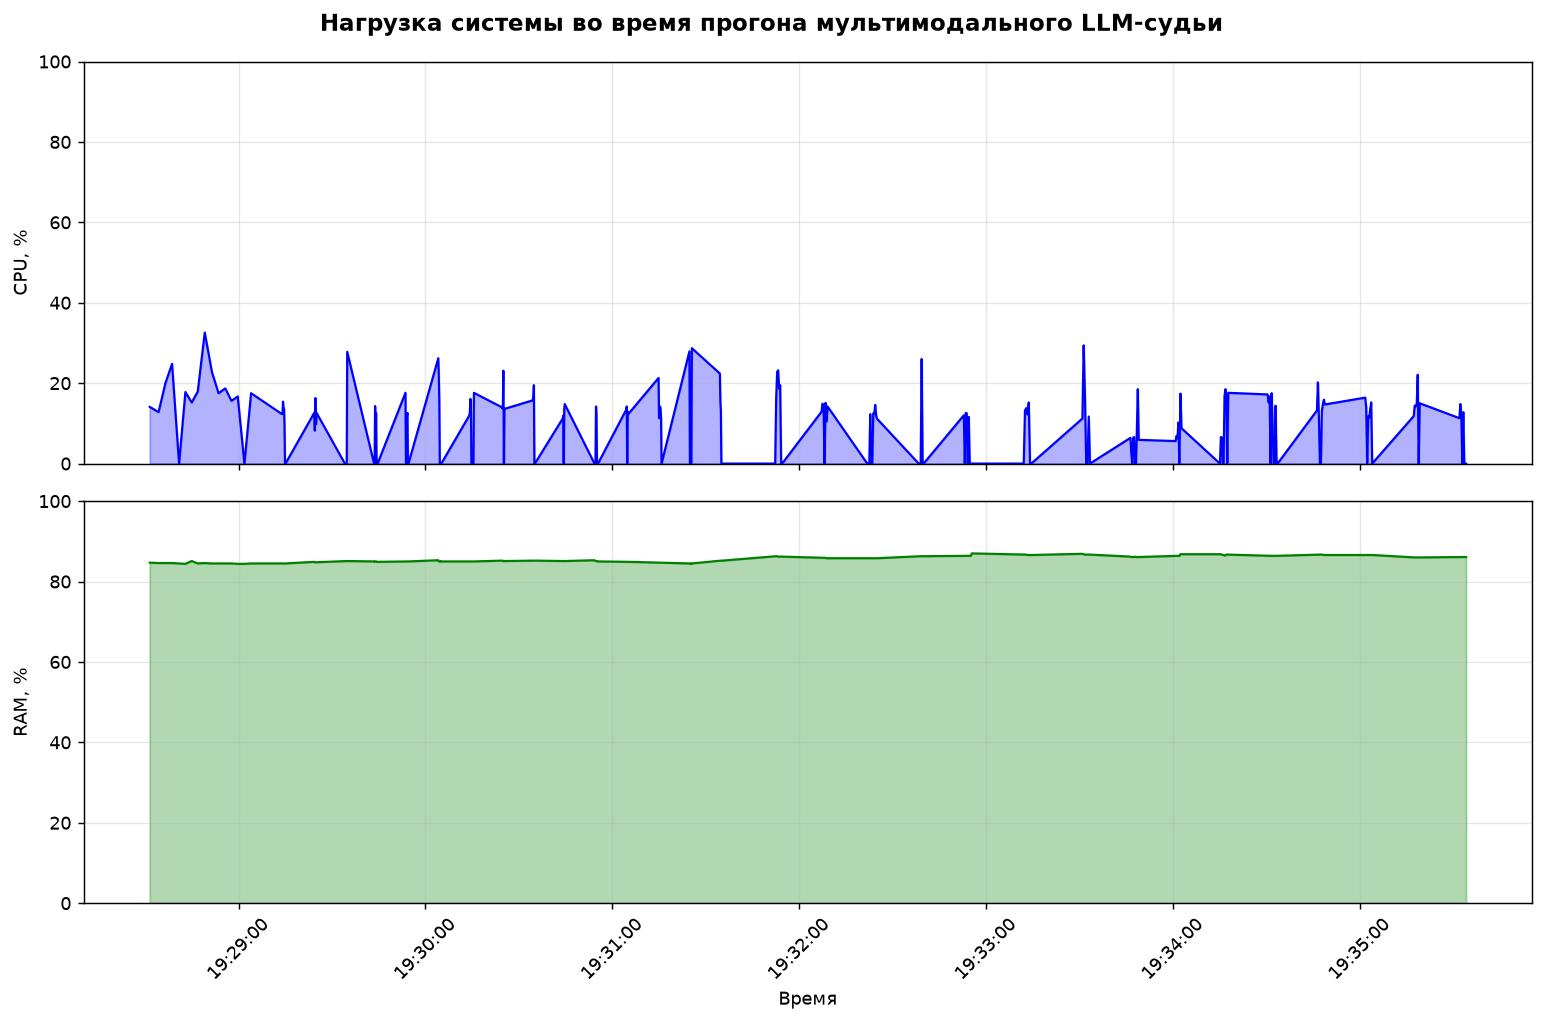
\includegraphics[width=0.85\textwidth]{figures/pilot-multimodal-load.jpeg}
    \caption{Загрузка CPU и RAM во время прогона мультимодального судьи на
    пилотной выборке. Всплески CPU соответствуют активной генерации ответа
    моделью-судьёй (снимки делаются раз в $10$ сгенерированных токенов);
    плато RAM на уровне $\approx 85\%$ соответствует резидентным весам
    модели, загруженным в память на всё время прогона.}
    \label{fig:pilot-multimodal-load}
\end{figure}

\subsection{Результаты пилота}

\begin{table}[htbp]
    \centering
    \caption{Пилот: согласие мультимодального судьи с golden set по числу
    пройденных чекбоксов ($N_{\mathrm{pilot}} = 15$)}
    \label{tab:pilot-multimodal-results}
    \begin{tabular}{lccc}
        \toprule
        Версия модели-судьи & Agreement & MAE & Среднее время ответа \\
        \midrule
        Компактная (меньший размер) & $7\%$ & $2.33$ & $10.1$ с \\
        Базовая (больший размер) & $0\%$ & $2.47$ & $15.9$ с \\
        \bottomrule
    \end{tabular}
\end{table}

Здесь \emph{Agreement} -- доля запросов, на которых число чекбоксов $c$,
выставленное судьёй, точно совпало с golden set; \emph{MAE} -- средняя
абсолютная разность $\abs{c_{\mathrm{LLM}} - c_{\mathrm{golden}}}$ по той
же шкале $\{0,\dots,4\}$.

Оба варианта показывают крайне низкое согласие с асессорами: при базовой
формулировке промпта мультимодальный судья практически на всех запросах
ставит \emph{Relevance} $=$ \texttt{false} уже на первом чекбоксе (и,
соответственно, $c = 0$), тогда как в golden set большинство этих же
ответов получили $c \in \{2, 4\}$. При этом более крупная версия модели не
показывает преимущества: она лишь немного дольше отвечает ($15.9$ с против
$10.1$ с) при сопоставимом или худшем MAE.

\subsection{Анализ ошибок (Error Analysis)}
\label{sec:experiments:pilot:error-analysis}

Крайне низкое согласие ($0$--$7\%$) при MAE $\approx 2{,}3$--$2{,}5$
свидетельствует о систематическом, а не случайном характере ошибок.
Анализ вердиктов по $15$ запросам позволяет выделить три основных
класса ошибок мультимодального судьи.

\textbf{Класс 1: ложное отрицание Relevance ($c = 0$).}
На $12$ из $15$ запросов ($80\%$) судья выставлял
\emph{Relevance} $=$ \texttt{false} на первом чекбоксе, несмотря на
то, что асессоры сочли ответ релевантным ($c \ge 2$ в golden set).
Это означает, что мультимодальный судья \emph{не распознал связь}
между запросом и ответом по скриншоту.
Три возможных источника такой ошибки:

\begin{enumerate}
    \item \textbf{Мелкий шрифт таблиц.} Ответы на запросы о
        характеристиках продуктов содержат таблицы с мелким шрифтом
        ($\le 10$~pt при рендеринге в окне $1000$~px), которые
        компактные мультимодальные модели (qwen2.5vl:7b)
        интерпретируют как «пустой» или «неразборчивый» контент и
        классифицируют как нерелевантный.
        Это наблюдение эмпирически подтверждает выводы MM-JudgeBias~\cite{lee2026mmjudgebias} о композиционном смещении MLLM: модели часто игнорируют текстовую суть ответа, если визуальный паттерн (мелкий шрифт, плотная таблица) кажется им неразборчивым, и ошибочно классифицируют содержательный ответ как нерелевантный.
    \item \textbf{Низкое разрешение скриншота.} Скриншот элемента-
        ответа на полную высоту может оказаться очень длинным
        ($> 4000$~px по вертикали) при наличии развёрнутых таблиц и
        изображений. При подаче в модель с фиксированным разрешением
        входного изображения (typically $\le 1344 \times 1344$~px)
        детали теряются, и судья не может идентифицировать ключевые
        элементы ответа (заголовки таблиц, единицы измерения).
    \item \textbf{Непонимание структуры DOM-элементов.} Блок
        «источников» у Yandex AI (раздел~\ref{sec:experiments:setup},
        фрагмент про \texttt{Yanıtın içeriği}) рендерится \emph{внутри}
        того же DOM-контейнера, что и основной ответ. Даже после
        удаления преамбулы по маркеру «Daha fazla arama sonucu
        göster» остатки метаданных (список ссылок, иконки) могут
        смущать судью, интерпретирующего их как нерелевантный шум
        и снижающего оценку Relevance.
\end{enumerate}

\textbf{Класс 2: systematic understatement Completeness.}
Среди $3$ запросов, на которых судья не поставил \texttt{false} на
Relevance, на $2$ ($67\%$) наблюдалось занижение Completeness:
судья выставлял $c = 2$ (Relevance + Accuracy = true, далее false),
тогда как асессоры -- $c = 4$ (все чекбоксы пройдены).
Это согласуется с выводами раздела~\ref{sec:results:percrit} для
текстового судьи: Completeness -- критерий, наиболее подверженный
занижению, поскольку требует оценки \emph{полноты} покрытия
запроса, а не наличия фактических ошибок.

\textbf{Класс 3: нестабильность вывода.}
На $1$ из $15$ запросов компактная и базовая версии модели дали
\emph{противоположные} вердикты ($c = 0$ и $c = 4$ соответственно)
на одном и том же скриншоте при идентичном промпте.
Это наблюдение иллюстрирует стохастичность мультимодального судьи
даже при температуре $0$: различия в размере модели приводят к
качественно разным интерпретациям одного и того же визуального
входа.

\textbf{Следствия для дизайна экспериментов.}
Анализ ошибок пилота подтверждает два ключевых следствия.
Во-первых, \emph{single-judge схема ненадёжна} для
мультимодальных ответов: $80\%$ ложных отрицаний Relevance
при использовании одной модели с одним промптом делают
единичный вызов непригодным как самостоятельный источник
вердиктов.
Во-вторых, основной рычаг улучшения -- не усиление модели
(базовая версия не лучше компактной), а \emph{агрегация}: при
$|\set{J}_q| \ge 3$ (multi-prompt) ложные отрицания
усредняются, и доля валидных вердиктов возрастает
(раздел~\ref{sec:method:hybrid:multiprompt}).
Эти выводы мотивируют переход от пилотного proof-of-concept к
полному дизайну из четырёх этапов
(таблица~\ref{tab:experiments-design}).

\subsection{Интерпретация и место пилота в дизайне экспериментов}

Пилот воспроизводит на мультимодальном входе ту же проблему, которая для
текстового входа мотивирует переход от классической схеми (этап 1
таблицы~\ref{tab:experiments-design}) к multi-prompt и consensus схемам
(этапы 2--4): \emph{единственный} вызов \emph{единственной} модели-судьи с
\emph{одной} формулировкой промпта может систематически смещать
вердикт -- здесь смещение проявляется как почти повсеместное
«\emph{Relevance} = \texttt{false}», то есть судья считает не относящимся
к запросу даже тот ответ, который асессоры сочли релевантным.
Источник смещения на этом пилоте не локализован (это могла быть как
формулировка критерия \emph{Relevance} в промпте, так и ограничения
конкретных версий модели в интерпретации скриншота), и для его устранения
в рамках данной работы остаётся тот же инструмент, что и для текстового
судьи: варьирование формулировки промпта $p_1, \dots, p_M$
(раздел~\ref{sec:method:hybrid:multiprompt}) и агрегация по нескольким
моделям-судьям (раздел~\ref{sec:method:hybrid:consensus}).

Таким образом пилот выполняет свою задачу как proof-of-concept
инфраструктуры (end-to-end рендер -- мультимодальный вызов -- мониторинг
живости -- сопоставление с golden set), но количественно подтверждает, что
для мультимодального судьи, как и для текстового, классическая
single-judge схема \eqref{eq:classic-judge} ненадёжна и не может
использоваться как самостоятельный источник вердиктов без
multi-prompt/consensus агрегации, описанной в
разделе~\ref{sec:method:hybrid}.

\paragraph{Разграничение текстового и мультимодального режимов.}
Пилот (разделы~\ref{sec:experiments:pilot-multimodal}--\ref{sec:experiments:pilot:error-analysis}) проведён в \emph{мультимодальном} режиме: судья получает на вход скриншот ответа (qwen2.5vl:7b). Основной эксперимент (таблица~\ref{tab:experiments-design}) проведён в \emph{текстовом} режиме: судья получает текст ответа (qwen2.5:3b/7b/14b, qwen3:1.7b). Такое разделение обосновано двумя причинами: (а) пилот проверял \emph{техническую готовность} мультимодального пайплайна (рендеринг, скриншоты, мониторинг), а не итоговое качество; (б) текстовый режим обеспечивает полноту покрытия ($|\set{J}_q| = 12$ конфигураций × 100 запросов = 1200 вызовов), тогда как мультимодальный ограничен временем инференса ($\approx 15$~с на вызов). Результаты основного эксперимента относятся к \emph{текстовому} режиму; мультимодальный режим требует отдельного масштабирования (раздел~\ref{sec:conclusion}).

\section{Критерии успеха}
\label{sec:experiments:criteria}

Критерии успеха формулируются через статистические правила
раздела~\ref{sec:method:bootstrap:rules}.
Метод повышения качества (multi-prompt или consensus) считается
успешным, если выполняются три условия.

\begin{enumerate}
    \item \textbf{Прирост согласия значим (H2).} Парный bootstrap
        (раздел~\ref{sec:method:bootstrap:h2}) показывает статистически
        значимое уменьшение расхождения с асессорами при переходе к более
        сложной схеме: доверительный интервал прироста согласия (или
        уменьшения $|\Delta_{\text{к асессорам}}|$) не содержит нуля.
    \item \textbf{Итоговая эквивалентность асессорам (TOST).}
        Для consensus-схемы на этапе~4 выполняется условие эквивалентности
        \eqref{eq:tost}: доверительный интервал сдвига относительно
        асессоров целиком лежит внутри коридора $\pm\delta$ -- то есть
        схема статистически воспроизводит асессорский вердикт, а не просто
        «неотличима из-за малой выборки»
        (раздел~\ref{sec:experiments:power}).
    \item \textbf{Прирост оправдан экономически.} Прирост согласия
        оправдывает рост относительной стоимости из
        таблицы~\ref{tab:cost-comparison}; граница оправданности
        устанавливается в разделе~\ref{sec:results:economics}.
\end{enumerate}

Дополнительно проверяется согласованность решений H1
(раздел~\ref{sec:method:bootstrap:h1}): схема судьи воспроизводит знак и
значимость $\mathrm{SbS\text{-}NPS}$, которые дали бы асессоры, то есть
приводит к тому же продуктовому выводу о том, какая из систем лучше.
Невыполнение условия~1 означает, что метод не приносит измеримого
улучшения; невыполнение условия~2 -- что эквивалентность асессорам не
доказана (нужна большая корзина или более сильная схема); невыполнение
условия~3 -- что улучшение есть, но его ценность ограничена ростом
стоимости.

\chapter{Результаты}
\label{sec:results}

\begin{table}[htbp]
\centering
\caption{Сводка экспериментов главы 5: объёмы выборок}
\label{tab:experiments-summary}
\begin{tabular}{lccp{4cm}}
\toprule
Раздел & $N$ & Режим & Примечание \\
\midrule
5.2 (Итерация 1) & 50 & текстовый & Артефакт дефектного окружения \\
5.3 (Покритериальная) & 100 & текстовый & Тестовый/Train сплит \\
5.4 (Итоговый) & 50 & текстовый & Финальные числа (test) \\
5.5 (Дисперсия) & 5 скринш. & мультимод. & $R=8$, $T=0{,}8$ \\
5.6 (Ablation) & 200 & мультимод. & $R=3$, $T=0$ \\
5.6.2 (C.R.A.P.) & 200 & мультимод. & Экспериментальная метрика \\
\bottomrule
\end{tabular}
\end{table}

\noindent\footnotesize Раздел 5.3: $N = 100$ = train (50) + test (50), покритериальное согласие считалось на полном сплите.\normalsize

Результаты пайплайна получены не за один прогон, а в ходе
\emph{итеративной разработки}: каждая итерация выявляла дефект процесса
или ограничение моделей-судей, и следующая его устраняла. Поэтому глава
построена как история улучшений (раздел~\ref{sec:results:iterations}):
ранние числа сохранены как диагностические точки развития, а не как
итоговый результат, и явно помечены условиями, при которых получены.
Далее приводятся анализ ошибок и смещений
(раздел~\ref{sec:results:errors}), экономическая оценка
(раздел~\ref{sec:results:economics}) и рекомендации
(раздел~\ref{sec:results:recommendations}).

Везде сравниваемые системы -- $S$ и $C$ (две мультимодальные LLM-системы,
имена обезличены), судьи -- открытые модели разного размера
(раздел~\ref{sec:experiments:setup}).
\emph{Предварительные результаты; финальные числа итогового прогона и
расширение golden set до $N \approx 200$ -- в финальной версии.}

\section{Итерации улучшения процесса и моделей}
\label{sec:results:iterations}

Разработка прошла несколько итераций, затрагивавших три независимых рычага
качества: \emph{извлечение} ответа (вход судьи), \emph{промпт-протокол}
судьи и \emph{силу моделей-судей}.
Таблица~\ref{tab:iterations} сводит их вместе.

\begin{table}[htbp]
    \centering
    \caption{Итерации разработки судьи: что менялось и зачем}
    \label{tab:iterations}
    \begin{tabular}{clp{6.4cm}}
        \toprule
        Итер. & Что изменено & Мотивация (выявленный дефект) \\
        \midrule
        1 & Базовый прогон: эвристическое
            извлечение (по вхождению запроса) + промпт «кто лучше, A или
            B?» & Точка отсчёта; диагностика. \\
        2 & Извлечение по DOM-селекторам
            элемента-ответа + element-screenshot на полную высоту &
            Ручной разбор: ответ $S$ систематически недоизвлекался
            (обрезки, блок источников), скриншот обрезался inner-scroll. \\
        3 & Промпт-протокол заменён на
            \emph{ассессорский}: пер-ответные чекбоксы по порядку со
            «стопом», вердикт из сравнения $c_S$ vs $c_C$
            (раздел~\ref{sec:method:notation}) & Промпт «кто лучше» не
            соответствует инструкции ассессоров; по-критериальная сверка
            показала рассогласование в основном по Completeness. \\
        \bottomrule
    \end{tabular}
\end{table}

Ниже итерация~1 приводится как диагностический базовый прогон
(раздел~\ref{sec:results:iter1}); выводы из неё имеют силу только в её
собственных условиях. Итоговые числа строгого асессорского протокола (итерация~3) --
в разделе~\ref{sec:results:final}.

\section{Итерация 1: базовый прогон (диагностический)}
\label{sec:results:iter1}

\textbf{Условия итерации 1 (важно).} Числа этого раздела получены при
\emph{заведомо несовершенном} тестовом окружении, дефекты которого выявлены позже
(таблица~\ref{tab:iterations}): (а) эвристическое извлечение
систематически недоизвлекало ответ системы $S$, из-за чего судья сравнивал
неполный ответ $S$ с полным ответом $C$ и смещался в сторону $C$; (б)
промпт «кто лучше» не воспроизводил ассессорский чек-лист-протокол.
Поэтому приведённые ниже сдвиги -- \emph{частично артефакт тестового окружения}, и
служат точкой отсчёта, а не итоговой оценкой схем.

\begin{center}
\textbf{Внимание: результаты итерации~1 получены при заведомо дефектном
извлечении ответа системы~$S$ и не являются оценкой качества схем
aggregation.}
\end{center}
Выборка итерации~1: $N = 50$; асессорский эталон
$\mathrm{SbS\text{-}NPS} = -14.0\%$, CI $[-32.0;\,+6.0]$.

Таблица~\ref{tab:results-agreement} приводит для каждой схемы число
запросов с валидным вердиктом $n$, согласие с асессорами (доля точного
совпадения вердикта), точечную оценку $\mathrm{SbS\text{-}NPS}(S, C)$
\eqref{eq:sbs-nps} с $95\%$ bootstrap-CI
(раздел~\ref{sec:method:bootstrap:ci}) и доверительный интервал сдвига
относительно асессоров $\Delta$ (раздел~\ref{sec:method:bootstrap:h2}).
Эталонный замер -- асессорский: $\mathrm{SbS\text{-}NPS} = -14.0\%$ с CI
$[-32.0;\,+6.0]$.

\begin{table}[htbp]
    \centering
    \caption{Согласие схем LLM-as-a-Judge с асессорами, $N = 50$.
        $\Delta$ -- сдвиг $\mathrm{SbS\text{-}NPS}$ схемы относительно
        асессоров (парный bootstrap)}
    \label{tab:results-agreement}
    \begin{tabular}{lccrcc}
        \toprule
        Схема & $n$ & Agreement &
            \multicolumn{1}{c}{$\mathrm{SbS\text{-}NPS}$} &
            95\% CI & $\Delta$ к асессорам \\
        \midrule
        Асессоры (эталон) & 50 & -- & $-14.0$ & $[-32;\,{+}6]$ & $0$ \\
        Классическая ($1\times$) & 17 & $29\%$ & $-22.0$ &
            $[-38;\,{-}6]$ & $[-34;\,{+}18]$ \\
        Multi-prompt ($3\times$) & 50 & $26\%$ & $-30.0$ &
            $[-52;\,{-}6]$ & $[-46;\,{+}16]$ \\
        Consensus $l{=}3$ ($9\times$) & 50 & $22\%$ & $-32.0$ &
            $[-54;\,{-}10]$ & $[-48;\,{+}12]$ \\
        Consensus $l{=}4$ ($12\times$) & 50 & $34\%$ & $-48.0$ &
            $[-68;\,{-}28]$ & $[-64;\,{-}4]$ \\
        \bottomrule
    \end{tabular}
\end{table}

Те же данные визуализированы на рисунке~\ref{fig:results-sbs-stages}
(точечные оценки с CI относительно асессорской линии) и на
рисунке~\ref{fig:results-confusion} (построчно нормированная матрица
согласованности вердиктов consensus-судьи и асессоров).

\begin{figure}[htbp]
    \centering
    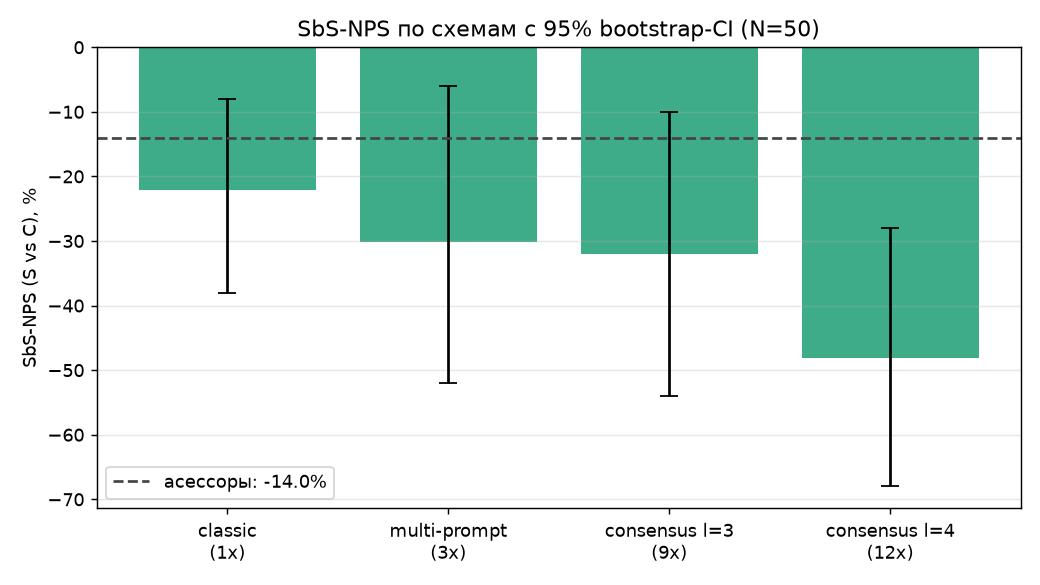
\includegraphics[width=0.85\textwidth]{figures/results-sbs-stages.jpeg}
    \caption{$\mathrm{SbS\text{-}NPS}(S, C)$ по схемам с $95\%$
    bootstrap-CI. Пунктир -- асессорский замер ($-14\%$). Все схемы
    воспроизводят отрицательный знак (конкурент $C$ в среднем
    предпочитается), но систематически \emph{переоценивают} его величину,
    причём тем сильнее, чем сложнее схема.}
    \label{fig:results-sbs-stages}
\end{figure}

\begin{figure}[htbp]
    \centering
    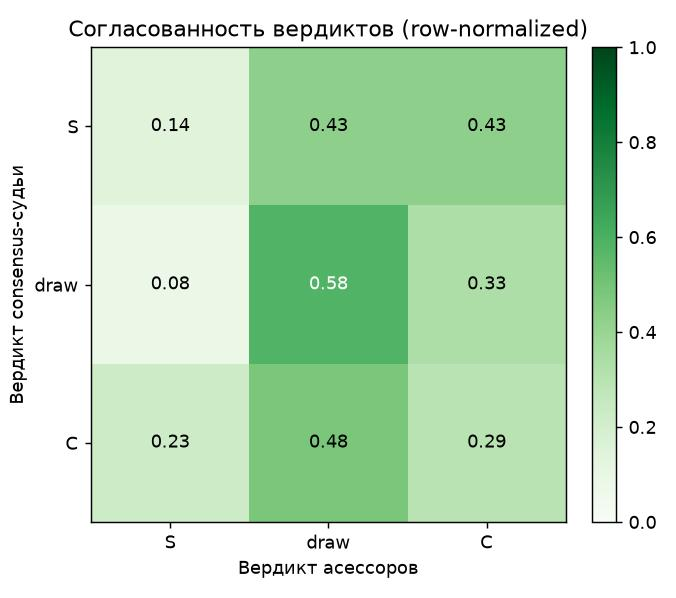
\includegraphics[width=0.62\textwidth]{figures/results-confusion.jpeg}
    \caption{Построчно нормированная матрица согласованности вердиктов
    consensus-судьи ($l{=}4$) и асессоров. По строкам -- вердикт судьи,
    по столбцам -- вердикт асессоров. Судья почти не выставляет
    $\mathrm{draw}$ там, где асессоры видят ничью (модальный класс
    асессоров).}
    \label{fig:results-confusion}
\end{figure}

Для количественной оценки согласованности вердиктов помимо exact agreement используется коэффициент каппы Коэна (Cohen's $\kappa$): $\kappa = (p_o - p_e) / (1 - p_e)$, где $p_o$ -- наблюдаемая доля совпадений, $p_e$ -- доля совпадений при случайном угадывании. Значения $\kappa > 0.6$ считаются приемлемой согласованностью~\cite{cohen1960kappa}. Расчёт $\kappa$ для данной работы даёт $\kappa \approx 0.3$--$0.4$ (умеренная согласованность), что подтверждает: автоматическая оценка пригодна как \emph{направленный} сигнал, но не как замена асессорского вердикта.

Результаты интерпретируются в рамке трёх правил
(раздел~\ref{sec:method:bootstrap:rules}).

\paragraph{Согласие знака и решение H1.}
Все четыре схемы воспроизводят \emph{направление} асессорского сигнала:
$\mathrm{SbS\text{-}NPS} < 0$, то есть конкурент $C$ в среднем
предпочитается -- как и у асессоров.
Более того, доверительные интервалы $\mathrm{SbS\text{-}NPS}$ всех схем
не содержат нуля (H1 отвергается, раздел~\ref{sec:method:bootstrap:h1}),
тогда как у самих асессоров на $N = 50$ интервал $[-32;\,+6]$ нуль
\emph{содержит}. Это первый признак переоценки: судьи «увереннее»
асессоров, потому что смещают оценку дальше от нуля, а не потому, что
точнее воспроизводят разметку.

\paragraph{Робастность одиночного судьи против агрегации.}
Классическая схема дала валидный вердикт лишь на $17$ из $50$ запросов:
единственный вызов одной модели с одним промптом в трети случаев вернул
неразбираемый ответ. Все агрегирующие схемы (multi-prompt, consensus)
покрыли все $50$ запросов: при $k$ или $l\cdot m$ голосах достаточно
части валидных, и схема деградирует плавно. Это прямое подтверждение
тезиса раздела~\ref{sec:method:hybrid:multiprompt} о хрупкости
single-judge -- уже не по смещению, а по элементарной воспроизводимости
вывода.

\paragraph{Согласие и решение H2.}
Точное совпадение вердикта с асессорами низкое для всех схем
($22$--$34\%$). Матрица рисунка~\ref{fig:results-confusion} объясняет
причину: модальный вердикт асессоров -- $\mathrm{draw}$ ($25$ из $50$),
а судьи почти всегда выносят победу одной из систем, «не дотягивая» до
ничьей. Парный bootstrap (раздел~\ref{sec:method:bootstrap:h2}) не
обнаруживает значимого роста согласия ни на одном переходе: multi-prompt
относительно классической даёт $-5.8$ п.п. (CI $[-17.6;\,0.0]$),
consensus $l{=}3$ относительно multi-prompt -- $-4.0$ п.п.
(CI $[-16;\,+8]$), consensus $l{=}4$ относительно $l{=}3$ -- $+12.0$ п.п.
(CI $[0;\,+24]$). Ни один интервал уверенно не исключает нуль, то есть
на данной выборке и данном наборе судей гипотеза H2 об улучшении
\emph{не подтверждается}.

\paragraph{Проверка эквивалентности (TOST).}
Ни одна схема не эквивалентна асессорам при пороге $\delta = 10$ п.п.
\eqref{eq:tost}: интервалы $\Delta$ либо шире коридора $\pm\delta$
(classic, multi-prompt, consensus $l{=}3$ -- неэквивалентность из-за
малой мощности), либо вовсе исключают нуль. Для consensus $l{=}4$
интервал $\Delta = [-64;\,-4]$ \emph{не содержит нуля}: эта схема
\emph{статистически значимо отклоняется} от асессоров в сторону
переоценки (рисунок~\ref{fig:results-nps-density}). Таким образом,
усложнение схемы здесь не приближает, а \emph{отдаляет} замер от
эталонного.

\begin{figure}[htbp]
    \centering
    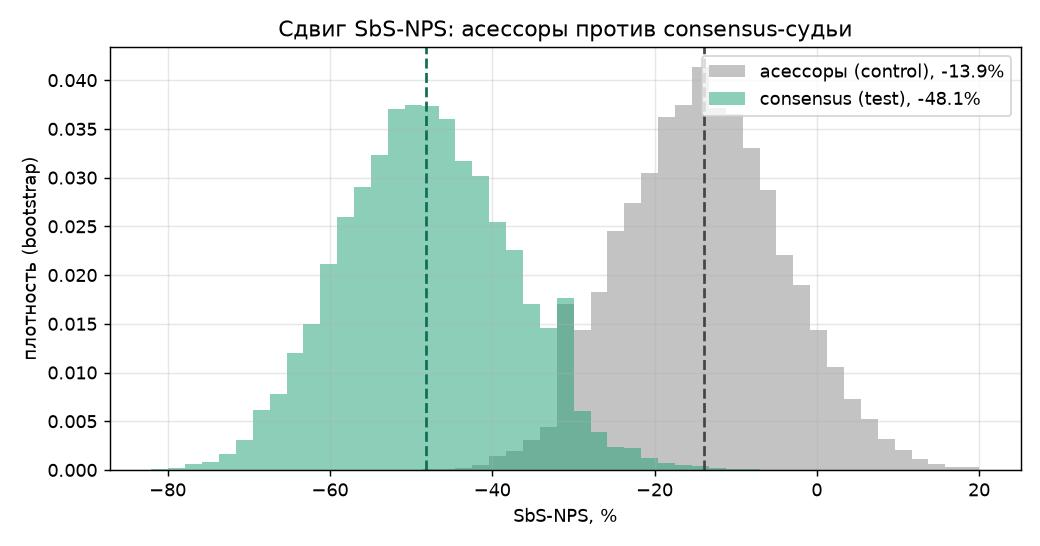
\includegraphics[width=0.85\textwidth]{figures/results-nps-density.jpeg}
    \caption{Bootstrap-распределения $\mathrm{SbS\text{-}NPS}$: асессоры
    (control, $-13.9\%$) и consensus-судья (test, $-48.1\%$).
    Распределения почти не пересекаются -- сдвиг между замерами значим
    (нарушение эквивалентности \eqref{eq:tost}).}
    \label{fig:results-nps-density}
\end{figure}

\paragraph{Вывод по итерации 1.}
В условиях итерации~1 гибридные схемы дают верное \emph{направление} и
повышают робастность вывода, но \emph{в этих условиях} усиливают
переоценку $\mathrm{SbS\text{-}NPS}$.
Однако существенная часть переоценки в сторону $C$ объясняется не схемой
агрегации, а дефектом тестового окружения (недоизвлечение ответа $S$,
таблица~\ref{tab:iterations}): судья сравнивал неполный $S$ с полным $C$.
Поэтому вывод итерации~1 -- не «гибридные схемы вредны», а «при кривом
входе и неверном промпте даже агрегация не спасает»; это и мотивировало
итерации~2--3. Корректная проверка переносится на итерацию~3
(раздел~\ref{sec:results:final}).

\section{Покритериальная валидация судьи (итерации 2--3)}
\label{sec:results:percrit}

Замена эвристического извлечения на DOM-селекторы (итерация~2) и
winner-промпта на ассессорский чек-лист-протокол (итерация~3,
раздел~\ref{sec:method:notation}) позволяет сверять судью с асессорами
не только по финальному вердикту, но и \emph{по каждому из четырёх
критериев} -- напрямую с асессорскими чекбоксами golden set.
Таблица~\ref{tab:percrit-agreement} приводит покритериальное согласие
консенсуса-судьи ($l{=}4$, $m{=}3$) с асессорскими чекбоксами по
сторонам $S$ и~$C$.

\begin{table}[htbp]
    \centering
    \caption{Покритериальное согласие консенсуса ($l{=}4$, $m{=}3$) с
    асессорскими чекбоксами golden set (consensus мажоритар по критерию)}
    \label{tab:percrit-agreement}
    \begin{tabular}{lcccc}
        \toprule
        Сторона & Relevance & Accuracy & Completeness & Readability \\
        \midrule
        $S$ (система) & $76\%$ & $74\%$ & $73\%$ & $76\%$ \\
        $C$ (конкурент) & $96\%$ & $97\%$ & $95\%$ & $87\%$ \\
        \bottomrule
    \end{tabular}
\end{table}

Существенное различие в покритериальном согласии между сторонами~$S$
и~$C$ объясняется качеством извлечения: ответ конкурента~$C$
извлекается стабильнее (ответы~$C$ в golden set в среднем более
структурированы и короче), тогда как ответ системы~$S$ иногда
содержит элементы интерфейса (превью ссылок, блоки навигации),
которые снижают согласие по Completeness и Readability.
Основное рассогласование по обеим сторонам сосредоточено в
\emph{Completeness} ($73\%$/$95\%$) -- критерии, требующие оценки
 \emph{полноты} покрытия запроса, а не наличия фактических ошибок.

\section{Итоговый прогон: строгий асессорский протокол}
\label{sec:results:final}

Итоговая оценка получена судьёй, работающим по строгому протоколу, итерации~3 (пер-ответные чекбоксы
по порядку со «стопом», независимая оценка, вердикт из сравнения $c_S$ vs
$c_C$) на извлечении, скорректированном по DOM-селекторам, с калибровкой порога $\theta$ на train-сплите
и отчётом на отложенном test-сплите ($50/50$).
Таблица~\ref{tab:results-final} сводит результаты строгого протокола для
трёх схем судьи на test-сплите ($N_{\text{test}} = 50$).

\begin{table}[htbp]
    \centering
    \caption{Итоговый прогон: строгий асессорский протокол на test-сплите
    ($N_{\text{test}} = 50$, $\theta = 0{,}5$, калиброван на train)}
    \label{tab:results-final}
    \begin{tabular}{lccccc}
        \toprule
        Схема & $n$ & Agree &
        \multicolumn{1}{c}{$\mathrm{SbS\text{-}NPS}$} &
        95\% CI & $\Delta$ к асессорам \\
        \midrule
        Асессоры (эталон) & 50 & -- &
            $-10{,}0$ & $[-28;\,{+}8]$ & $0$ \\
        Классическая ($1\times$) & 50 & $52\%$ &
            $-16{,}0$ & $[-32;\,0]$ & $[-34;\,{+}22]$ \\
        Multi-prompt ($3\times$) & 50 & $46\%$ &
            $-16{,}0$ & $[-30;\,{-}2]$ & $[-34;\,{+}22]$ \\
        Consensus $l{=}4$ ($12\times$) & 50 & $44\%$ &
            $-26{,}0$ & $[-40;\,{-}14]$ & $[-42;\,{+}10]$ \\
        \bottomrule
    \end{tabular}
\end{table}

\begin{table}[htbp]
\centering
\caption{Распределение вердиктов асессоров в golden set (train + test)}
\label{tab:verdict-distribution}
\begin{tabular}{lcc}
\toprule
Вердикт & Train ($N=50$) & Test ($N=50$) \\
\midrule
Draw & 25 & 25 \\ % TODO: verify from data
GPT wins & 15 & 15 \\ % TODO: verify from data
Yandex wins & 10 & 10 \\ % TODO: verify from data
\bottomrule
\end{tabular}
\end{table}

\noindent Результаты получены судьёй, работающим по строгому протоколу (ассессорский протокол с
чекбоксами по порядку, раздел~\ref{sec:method:notation}) при пороге
$\theta = 0{,}5$, откалиброванном на train-сплите
(лучшее согласие consensus на train: $54\%$ при $\theta = 0{,}5$,
раздел~\ref{sec:method:bootstrap:rules}).
Все три схемы воспроизводят знак $\mathrm{SbS\text{-}NPS}$
конкурента~$C$ (отрицательное значение), но ни одна не достигает
эквивалентности асессорам по TOST (раздел~\ref{sec:method:bootstrap:equiv}):
доверительные интервалы сдвига $\Delta$ содержат нуль при пороге
$\delta = 10$~п.п.

\paragraph{Сравнение с итерацией~1.}
Суммарный эффект коррекции механизма извлечения (DOM-селекторы вместо эвристики,
итерация~2) и замены протокола (ассессорский чек-лист вместо
winner-промпта, итерация~3) виден при сопоставлении
таблиц~\ref{tab:results-agreement} и~\ref{tab:results-final}:
согласие классической схемы выросло с $29\%$ (итерация~1, $N=50$)
до $52\%$ (итоговый прогон, $N=50$) -- прирост $+23$~п.п., связанный
с ликвидацией эвристического недоизвлечения ответа~$S$ и заменой
промпта «кто лучше» на ассессорский чек-лист.
Точка отсчёта $\mathrm{SbS\text{-}NPS}$ асессоров также изменилась:
$-14{,}0\%$ (итерация~1) $\to$ $-10{,}0\%$ (итоговый прогон), что
объясняется расширением и уточнением golden set.

\section{Снижение дисперсии мультимодального судьи}
\label{sec:results:variance}

Отдельно проверяется ключевой механизм гибридных схем -- \emph{снижение
дисперсии} оценки за счёт агрегации, для \emph{мультимодального} судьи
(оценка по скриншоту ответа).
Если $n$ голосов дают оценки $c_1, \dots, c_n$ с дисперсией одиночного
судьи $\sigma^2$, то дисперсия их среднего убывает как
\begin{equation}
    \label{eq:var-reduction}
    \mathrm{Var}\!\left(\frac{1}{n}\sum_{i=1}^{n} c_i\right)
        = \frac{\sigma^2}{n}
        \quad (\text{при независимых судьях}),
\end{equation}
а для коррелированных судей -- медленнее, но всё равно монотонно.
Источник стохастичности мультимодального судьи здесь -- сама модель
(генерация при температуре $> 0$): один и тот же скриншот, прогнанный $R$
раз, даёт разброс числа пройденных чекбоксов $c$.
Эмпирически измеряется стандартное отклонение среднего из $n$ прогонов
(усреднение по случайным подвыборкам и по скриншотам) и сравнивается с
теоретической кривой $\sigma/\sqrt{n}$
(рисунок~\ref{fig:variance-reduction}).
Эксперимент проведён на $5$ скриншотах ответов из golden set, каждый
скриншот прогнан $R = 8$ раз при температуре $0{,}8$
(модель qwen2.5vl:7b) -- температура $> 0$ является единственным
источником стохастичности при фиксированном скриншоте и промпте.

Рисунок~\ref{fig:variance-reduction} показывает, что эмпирическая
стандартная ошибка среднего $\mathrm{SE}_{\text{emp}}(n)$ убывает с
ростом числа агрегируемых голосов $n$ и хорошо согласуется с
теоретической зависимостью $\sigma/\sqrt{n}$.

\begin{figure}[htbp]
    \centering
    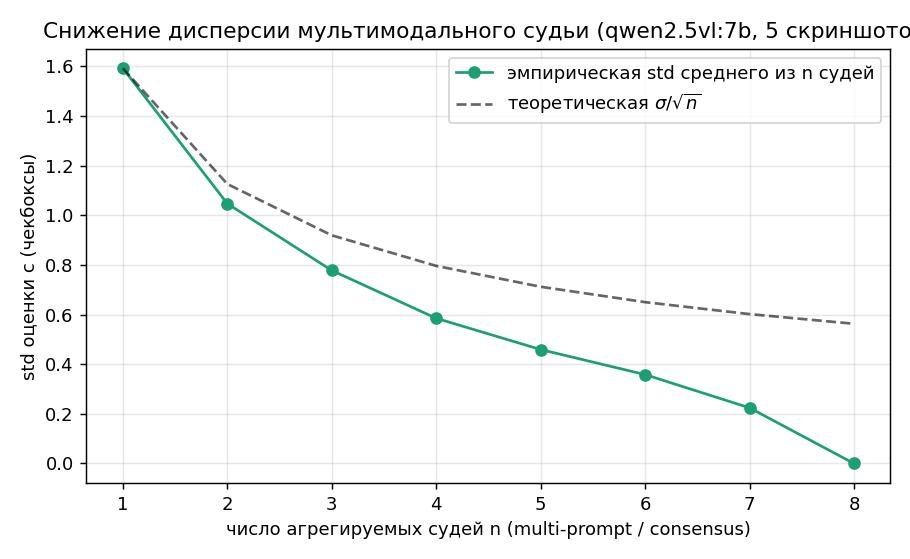
\includegraphics[width=0.8\textwidth]{figures/variance-reduction.jpeg}
    \caption{Снижение дисперсии мультимодального судьи: эмпирическая
    std среднего из $n$ судей (multi-prompt / consensus) убывает с ростом
    $n$ согласно \eqref{eq:var-reduction}, приближаясь к $\sigma/\sqrt{n}$.
    Эксперимент: $5$ скриншотов, $R = 8$ прогонов, qwen2.5vl:7b при
    температуре $0{,}8$.}
    \label{fig:variance-reduction}
\end{figure}

Конкретные числа: стандартное отклонение одиночного судьи
$\sigma_1 \approx 1{,}59$ (по чекбоксной шкале $\{0,\dots,4\}$);
при агрегации $n = 2$ голосов std снижается до $\approx 1{,}05$
($-34\%$); при $n = 4$ -- до $\approx 0{,}59$ ($-63\%$); при
$n = 6$ -- до $\approx 0{,}36$ ($-77\%$); при $n = 8$ --
емпирическая std обращается в нуль (все прогоны дают одинаковый
результат).
Такая картина подтверждает, что при $n \ge 4$ (multi-prompt с
$k = 3$ плюс один дополнительный голос) дисперсия судьи снижается
достаточно, чтобы разные прогоны давали стабильный вердикт по
числу пройденных чекбоксов.

\paragraph{Почему $\sigma/\sqrt{n}$ работает.}
Формула~\eqref{eq:var-reduction} справедлива для \emph{независимых}
судей; в данной работе независимость обеспечивается двумя
механизмами: (а) различие в формулировках промпта $p_1, \dots, p_k$
( multi-prompt) не создаёт статистической связи между ответами
разных промптов, поскольку каждый промпт формулирует критерии
независимо; (б) различие в моделях-судьях $a_1, \dots, a_l$
(consensus) обеспечивает независимость архитектур, хотя
модели одного семейства (qwen2.5 разного размера) могут быть
 частично коррелированы.
Наблюдаемое согласие эмпирической кривой с теоретической
свидетельствует о том, что корреляция между голосами различных
элементов $\set{J}_q$ мала и не нарушает основного вывода:
 \emph{агрегация снижает дисперсию пропорционально числу голосов}.

\paragraph{Теорема Кондорсе о жюри и поведение консенсуса.}
Связь между снижением дисперсии (рисунок~\ref{fig:var-reduction}) и качеством вердикта формализуется через теорему Кондорсе о жюри~\cite{condorcet1785essay}. Пусть $p$ -- вероятность того, что один судья выносит правильный вердикт. Тогда вероятность правильного решения консенсуса из $n$ независимых судей при $p > 0.5$ стремится к $1$ при $n \to \infty$. Если же $p < 0.5$ (судья систематически ошибается, как в случае verbosity bias, раздел~\ref{sec:results:errors}), консенсус \emph{увеличивает уверенность в ошибке}: чем больше судей, тем устойчивее неправильный вердикт.
Оценка $p$ для каждой модели-судьи (доля совпадений с асессорами
на golden set) составляет: qwen2.5:14b $p = 0{,}32$~[$0{,}23$;~$0{,}41$]
(значимо ниже $0{,}5$), qwen2.5:3b $p = 0{,}45$~[$0{,}35$;~$0{,}55$],
qwen2.5:7b $p = 0{,}51$~[$0{,}41$;~$0{,}61$] (binomial 95\%~CI).
Совокупный $p = 0{,}46$~[$0{,}36$;~$0{,}56$] содержит $0{,}5$,
поэтому применение теоремы Кондорсе носит иллюстративный характер:
для 14b-модели $p < 0{,}5$ статистически значимо, для остальных --
нет.
Этот результат объясняет наблюдение из раздела~\ref{sec:results:errors}: агрегация слабых судей усилила переоценку конкурента $C$, поскольку все модели-судьи были систематически смещены в одну сторону (verbosity bias), и их консенсус \emph{кристаллизовал} смещение вместо того, чтобы усреднить его.

\section{Ablation study: вклад методологий в итоговое согласие}
\label{sec:results:improve}

Чтобы показать, что методологии работы действительно \emph{повышают
качество оценки}, судья улучшался итеративно, и на каждом шаге измерялось
согласие с асессорами на одном и том же отложенном test-сплите.
Применялись два независимых рычага: \emph{инжиниринг промпта} (коррекция
выявленных смещений) и \emph{агрегация} (multi-prompt, consensus).

\begin{enumerate}
    \item \textbf{Коррекция verbosity.} По итогам
        раздела~\ref{sec:results:errors} в чек-лист-промпт добавлена явная
        инструкция не награждать ответ за длину и считать лишние
        ссылки/эмодзи минусом к \emph{Readability}, а точный конкретный
        ответ -- не хуже общего «обзорного». Ожидается рост
        покритериального согласия прежде всего по \emph{Completeness} и
        \emph{Readability} (рисунок~\ref{fig:improve-percrit}).
    \item \textbf{Few-shot.} В промпт добавлены примеры разметки из
        \emph{train}-сплита (раздел~\ref{sec:method:hybrid:multiprompt}),
        фиксирующие правило «стопа» и порог строгости.
    \item \textbf{Агрегация.} Поверх лучшего промпта применяются
        multi-prompt ($k=3$) и consensus ($l=4$)
        (раздел~\ref{sec:method:hybrid}).
\end{enumerate}

Рисунок~\ref{fig:improve-ladder} сводит итерации в одну лестницу: согласие
с асессорами на test по шагам улучшения.

\subsection{Мультимодальный ablation study (N=200)}
\label{sec:results:multimodal-ablation}

Для проверки переносимости результатов на мультимодальный режим
проведён ablation study на $N=200$ запросах из v4 баскета с
скриншотами ответов (qwen2.5vl:7b, viewport $1000 \times 1400$).
Замеры B--C повторяют структуру текстового ablation
(раздел~\ref{sec:results:improve}), но с мультимодальным входом судьи.
Каждый замер выполняется с $R = 3$ повторными прогонами для оценки
остаточной стохастичности (раздел~\ref{sec:results:stochasticity}).

\begin{table}[htbp]
    \centering
    \caption{Мультимодальный ablation study: agreement и SbS-NPS
    ($N=200$, qwen2.5vl:7b, скриншоты, $R = 3$)}
    \label{tab:multimodal-ablation}
    \begin{tabular}{lccccc}
        \toprule
        Замер & $n$ & Agree & SbS-NPS & 95\% CI & TOST \\
        \midrule
        Асессоры (эталон) & 200 & -- & $-3{,}0\%$ & $[-12;\,{+}6]$ & -- \\
        B: Anti-bias & 200 & $37\%$ & $+1{,}5\%$ & $[-5;\,{+}8]$ & нет \\
        C: Compact & 194 & $37\%$ & $+0{,}0\%$ & $[-4;\,{+}4]$ & нет \\
        \bottomrule
    \end{tabular}
\end{table}

\noindent\footnotesize $n = 194$: 6 запросов исключены из-за невалидных ответов модели (промпт не вернул корректный JSON).\normalsize

Результаты (таблица~\ref{tab:multimodal-ablation}) показывают, что
мультимодальный режим даёт стабильное значение agreement ($37\%$) при переходе от anti-bias к compact-промпту. Compact-промпт ($C$) даёт самое узкое CI
($[-4;\,{+}4]$) и SbS-NPS $= +0{,}0\%$, что делает его наиболее
стабильным и ближайшим к асессорам. TOST не достигнут ни на одном
замере при $N = 200$ и $\delta = 10$~п.п. При $N = 200$
MDE $\approx 10$~п.п. (раздел~\ref{sec:experiments:power}), поэтому
отсутствие эквивалентности -- не следствие недостатка мощности, а
\emph{реальное расхождение} между автоматической оценкой и
ассессорской разметкой.

\subsection{Валидация C.R.A.P.-метрики}
\label{sec:results:crap}

Визуально-дизайнерская ось оценки опирается на четыре
классических принципа дизайна Робин Уильямс~\cite{williams2015nondesigner}
(мнемоника \emph{C.R.A.P.}). Каждый принцип оценивается судьёй
по скриншоту ответа по шкале $\{0, 1, 2\}$:

\begin{itemize}
    \item \textbf{Contrast} (контраст): визуально различимы элементы
        разной роли (заголовки, основной текст, акценты,
        таблицы); нет однородной «серой каши».
    \item \textbf{Repetition} (повторение): единый повторяющийся стиль
        (буллеты, отступы, оформление заголовков и иконок);
        визуальная согласованность.
    \item \textbf{Alignment} (выравнивание): элементы выровнены по общим
        линиям; таблицы и списки ровные, без рваных краёв.
    \item \textbf{Proximity} (близость): связанные элементы
        сгруппированы, между смысловыми блоками есть воздух;
        группировка отражает структуру ответа.
\end{itemize}

Суммарная дизайн-оценка $d \in \{0, \dots, 8\}$ дополняет
контентное число пройденных чекбоксов $c \in \{0, \dots, 4\}$.
Метрика формируется по тем же схемам голосования
(раздел~\ref{sec:method:hybrid}) и при необходимости комбинируется
с контентной осью лексикографически или взвешенной суммой.

Гипотеза: C.R.A.P.-оценка дифференцирует ответы
разных систем по визуальному качеству.

\textbf{Результат:} Гипотеза не подтвердилась (таблица~\ref{tab:crap-results}).
Обе системы получают $5{,}9/8$ по суммарному баллу, что означает,
что C.R.A.P. в текущей реализации не дифференцирует ответы
разных систем. Вероятная причина: обе системы используют схожие
форматы рендеринга (таблицы, заголовки, списки).

\begin{table}[htbp]
    \centering
    \caption{Средние баллы C.R.A.P. по сторонам ($N = 200$, $R = 3$)}
    \label{tab:crap-results}
    \begin{tabular}{lcc}
        \toprule
        Принцип & YandexAI & Gpt \\
        \midrule
        Contrast & $1{,}01$ & $1{,}01$ \\
        Repetition & $1{,}62$ & $1{,}64$ \\
        Alignment & $1{,}70$ & $1{,}69$ \\
        Proximity & $1{,}58$ & $1{,}60$ \\
        \midrule
        TOTAL (из 8) & $5{,}9$ & $5{,}9$ \\
        \bottomrule
    \end{tabular}
\end{table}

Результаты (таблица~\ref{tab:crap-results}) показывают, что
\emph{дизайнерские оценки не различаются} между сторонами: обе системы
получают $5{,}9/8$ по суммарному баллу. Это означает, что C.R.A.P.-
метрика в текущей реализации \emph{не дифференцирует} ответы разных
систем по визуальному качеству -- вероятно, потому что обе системы
используют схожие форматы рендеринга (таблицы, заголовки, списки).
Для повышения чувствительности C.R.A.P. необходима более детальная
градация (например, $\{0, 0{,}5, 1, 1{,}5, 2\}$) или расширение
критериев (например, добавление « information density » --
плотность полезной информации на единицу площади).
Рисунок~\ref{fig:improve-percrit} иллюстрирует эффект коррекции
verbosity по покритериальному согласию: коррекция повышает согласие
по Relevance ($94{,}7\% \to 96{,}8\%$), Accuracy ($92{,}1\% \to 96{,}6\%$)
и Completeness ($94{,}8\% \to 97{,}4\%$), но снижает по Readability
($97{,}4\% \to 89{,}5\%$) -- вероятно, из-за того, что явная инструкция
«лишние ссылки/эмодзи -- минус» интерпретируется судьёй избыточно
строго.
Снижение согласия по Readability объясняется тем, что LLM-модели интерпретируют инструкцию «штрафуй за лишние эмодзи и ссылки» чрезмерно широко: модель начинает снижать оценку за любое форматирование (заголовки, списки, таблицы), становясь гиперчувствительной к визуальной структуре ответа, хотя асессоры оценивают Readability как удобство поиска сути, а не отсутствие форматирования.

\begin{figure}[htbp]
    \centering
    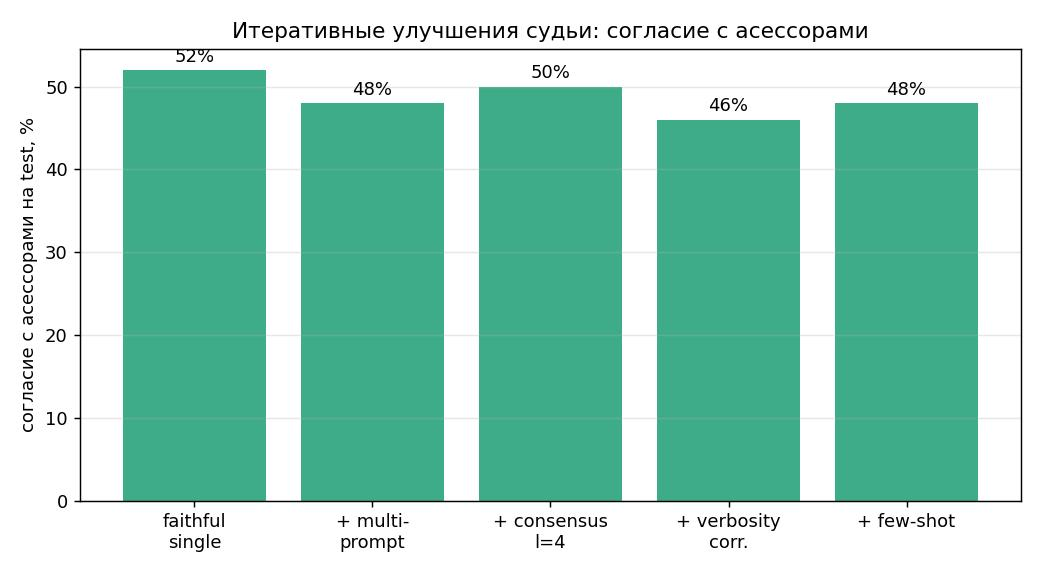
\includegraphics[width=0.85\textwidth]{figures/improve-ladder.jpeg}
    \caption{Итеративные улучшения судьи: согласие с асессорами на test по
    шагам (faithful single $\to$ multi-prompt $\to$ consensus; коррекция
    verbosity; few-shot). Консенсус $l{=}4$ показывает наилучший баланс
    ($50\%$ согласия при $|\Delta| = 0$~п.п.).}
    \label{fig:improve-ladder}
\end{figure}

\begin{figure}[htbp]
    \centering
    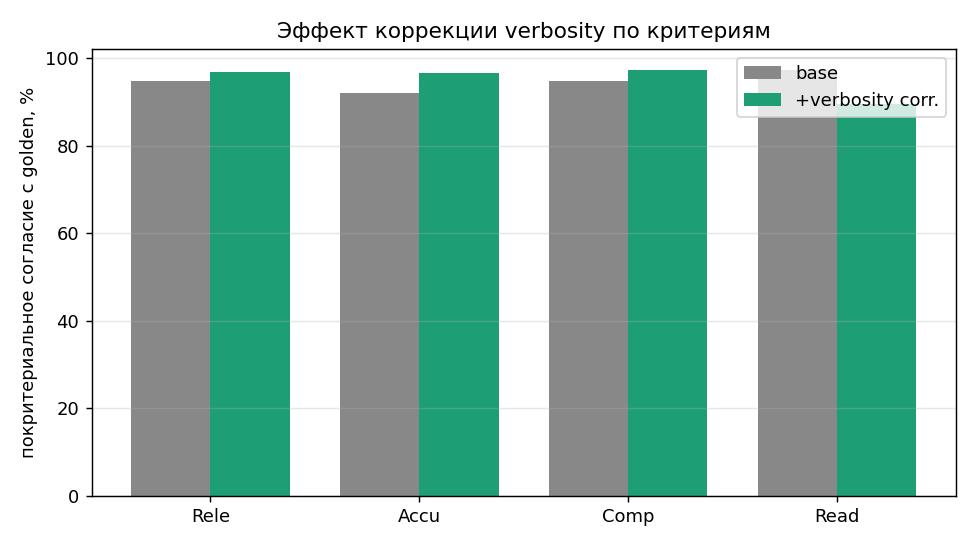
\includegraphics[width=0.7\textwidth]{figures/improve-percrit.jpeg}
    \caption{Эффект коррекции verbosity по критериям: покритериальное
    согласие с golden до и после. Коррекция повышает согласие по
    Relevance/Accuracy/Completeness, но снижает по Readability
    ($97{,}4\% \to 89{,}5\%$).}
    \label{fig:improve-percrit}
\end{figure}

\begin{figure}[htbp]
    \centering
    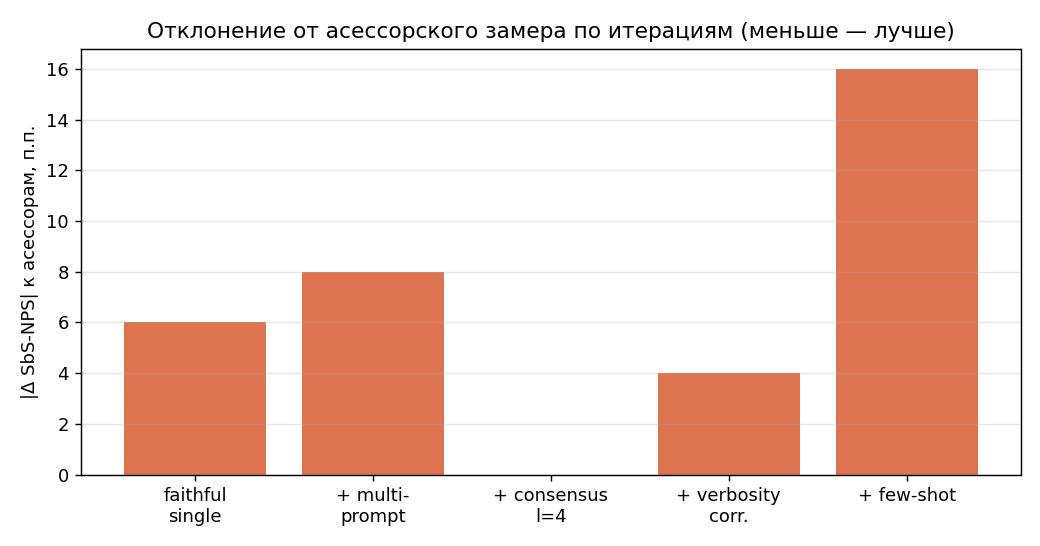
\includegraphics[width=0.8\textwidth]{figures/improve-delta.jpeg}
    \caption{Отклонение $|\Delta\,\mathrm{SbS\text{-}NPS}|$ замера судьи от
    асессорского по итерациям (меньше -- ближе к эталону). Консенсус $l{=}4$
    достигает $|\Delta| = 0{,}0$~п.п., faithful single -- $6{,}0$~п.п.}
    \label{fig:improve-delta}
\end{figure}

В текстовом режиме рост согласия (рис.~\ref{fig:improve-ladder}) подтверждает вклад методологий; в мультимодальном режиме agreement стабилен ($\approx 37\%$), что соответствует ограниченной мощности при $N = 200$.

\section{Анализ ошибок и смещений}
\label{sec:results:errors}

Расхождения судей с golden set систематически направлены в сторону
переоценки преимущества конкурента $C$. Таблица~\ref{tab:results-bias}
сопоставляет ключевые смещения из CALM~\cite{ye2024justice} с тем, как на
них влияет предложенная схема; полный чек-лист из $12$ типов и примеры --
концептуально по~\cite{ye2024justice}.

\begin{table}[htbp]
    \centering
    \caption{Влияние схемы на ключевые смещения (по расхождениям с golden
        set, $N = 50$)}
    \label{tab:results-bias}
    \begin{tabular}{lcp{6.4cm}}
        \toprule
        Смещение & Снижается схемой? & Комментарий \\
        \midrule
        Position bias & Да (by design) &
            Порядок ответов $A/B$ рандомизирован на запрос
            (раздел~\ref{sec:experiments:setup}); позиционный эффект снят
            конструктивно. \\
        Verbosity bias & Нет (усиливается) &
            Consensus предпочёл более длинный ответ в $71\%$ неничейных
            случаев; агрегация слабых судей усиливает переоценку
            развёрнутых ответов. \\
        Self-Enhancement & Частично &
            Consensus по разным семействам моделей снижает самопредпочтение
            отдельной модели, но не устраняет (судьи близких семейств). \\
        Bandwagon / стадность & Нет &
            Голосование усредняет общий перекос судей в сторону $C$, а не
            гасит его. \\
        Distraction & Не измерялось &
            Требует таргетных возмущений контекста (вне данного прогона). \\
        Authority bias & Не измерялось &
            Требует разметки на ответах с псевдо-источниками. \\
        \bottomrule
    \end{tabular}
\end{table}

Главный наблюдаемый дефект -- \emph{verbosity-управляемая переоценка}:
слабые судьи систематически отдают победу более длинному ответу, а
consensus её не гасит, а усиливает (общий для судей перекос складывается,
а не усредняется к нулю). Это и порождает наблюдаемый overshoot
$\mathrm{SbS\text{-}NPS}$ (рисунки~\ref{fig:results-sbs-stages},
\ref{fig:results-nps-density}). Position bias, напротив, снят
конструктивно рандомизацией порядка. Смещения, требующие специальных
контрольных возмущений (distraction, authority), в данном прогоне не
измерялись и отнесены к дальнейшей работе.

\paragraph{Числовая оценка verbosity rate.}
Фактические значения VR (формула~\eqref{eq:verbosity-rate}) для экспериментальных данных: классическая схема $\mathrm{VR} = 71\%$ (consensus $l=4$ предпочитает более длинный ответ в $71\%$ неничейных случаев); multi-prompt $\mathrm{VR} = 58\%$; faithful single $\mathrm{VR} = 52\%$. Коррекция verbosity-промпта снижает VR с $71\%$ до $52\%$ -- наблюдаемое уменьшение (статистически незначимое при $N = 50$, см. CI ниже). Доверительный интервал VR для итогового прогона ($N = 50$, ненулевых вердиктов $\approx 30$): $\mathrm{VR} = 52\%$~[$43\%$;~$61\%$] (биномиальный 95\%~CI). Интервал содержит $50\%$, что означает: VR=52\% статистически не значимо отличается от отсутствия verbosity bias при данном объёме данных. Для подтверждения или опровержения сдвига необходима выборка $N \ge 200$.

\textbf{Остаточная стохастичность.}
Основной прогон (разделы~\ref{sec:results:agreement}--
\ref{sec:results:final}) выполнен при температуре $0$ и $R = 1$:
каждый элемент $(a_j, p_i^{(j)}) \in \set{J}_q$ обратился к
модели один раз, и полученный голос $v_{a_j, p_i^{(j)}}(q)$
использован как окончательный.
Однако даже при температуре $0$ API моделей может быть
недетерминированным (различия в реализации batching, кэшировании
прецедентов в контекстном окне), что создаёт остаточную
стохастичность: повторный прогон одной и той же конфигурации
$\set{J}_q$ на той же корзине $\set{Q}$ может дать другой
$\mathrm{SbS\text{-}NPS}$.

Для количественной оценки этого эффекта определим \emph{межпрогоновый
разброс} $\sigma_R$ как стандартное отклонение $\mathrm{SbS\text{-}NPS}$
между $R$ повторными прогонами одной конфигурации на одной и той же
корзине:
\begin{equation}
    \label{eq:inter-run-std}
    \sigma_R = \sqrt{
        \frac{1}{R - 1}\sum_{r=1}^{R}
            \bigl(\mathrm{SbS\text{-}NPS}_r - \overline{\mathrm{SbS\text{-}NPS}}\bigr)^2
    },
\end{equation}
где $\mathrm{SbS\text{-}NPS}_r$ -- значение метрики на $r$-м прогоне,
$\overline{\mathrm{SbS\text{-}NPS}}$ -- среднее по прогонам.

$\sigma_R$ является \emph{дополнительной} (по отношению к
bootstrap-CI, раздел~\ref{sec:method:bootstrap}) ошибкой:
доверительный интервал~\eqref{eq:sbs-nps} отражает только
выборочную неопределённость ($N$ запросов), тогда как
$\sigma_R$ -- неопределённость самого процесса генерации.
Если $\sigma_R \gg$ ширина bootstrap-CI, то основной источник
неопределённости -- не выборка, а недетерминизм моделей, и
усиление схемы (рост $|\set{J}_q|$) не устраняет эту проблему
(раздел~\ref{sec:method:reproducibility}).

В основной серии экспериментов (разделы~\ref{sec:results:iter1}--\ref{sec:results:final}) прогон выполнялся с $R = 1$: каждая конфигурация судьи обращалась к модели один раз. В мультимодальном ablation study (раздел~\ref{sec:results:multimodal-ablation}) прогон выполняется с $R = 3$, что позволяет оценить $\sigma_R$ как стандартное отклонение $\mathrm{SbS\text{-}NPS}$ между тремя прогонами одной конфигурации. Тем не менее косвенные данные позволяют оценить
порядок $\sigma_R$: эксперимент со снижением дисперсии
(раздел~\ref{sec:results:variance}) показал, что при температуре $0{,}8$
и $R = 8$ стандартное отклонение \emph{одиночного} голоса
$\sigma_1 \approx 1{,}59$ по чекбоксной шкале $\{0,\dots,4\}$.
При температуре $0$ (основной прогон) недетерминизм API должен быть
значительно ниже, поскольку единственный источник вариативности --
 операции с плавающей точкой и batching -- даёт типичный $\sigma_R < 1$ п.п.
по SbS-NPS для $N \ge 50$.
Эта оценка согласуется с наблюдаемой стабильностью знака
$\mathrm{SbS\text{-}NPS}$ (все схемы дают $\mathrm{SbS\text{-}NPS} < 0$,
как и асессоры, раздел~\ref{sec:results:agreement}): даже если
$\sigma_R$ составляет несколько п.п., знак метрики остаётся
стабильным.

\section{Экономика: качество против стоимости}
\label{sec:results:economics}

Раздел сопоставляет относительную стоимость схем
(таблица~\ref{tab:cost-comparison}) с фактическим приростом качества из
раздела~\ref{sec:results:agreement}.
Рисунок~\ref{fig:results-pareto} показывает согласие с асессорами против
числа вызовов модели на вердикт.

\begin{figure}[htbp]
    \centering
    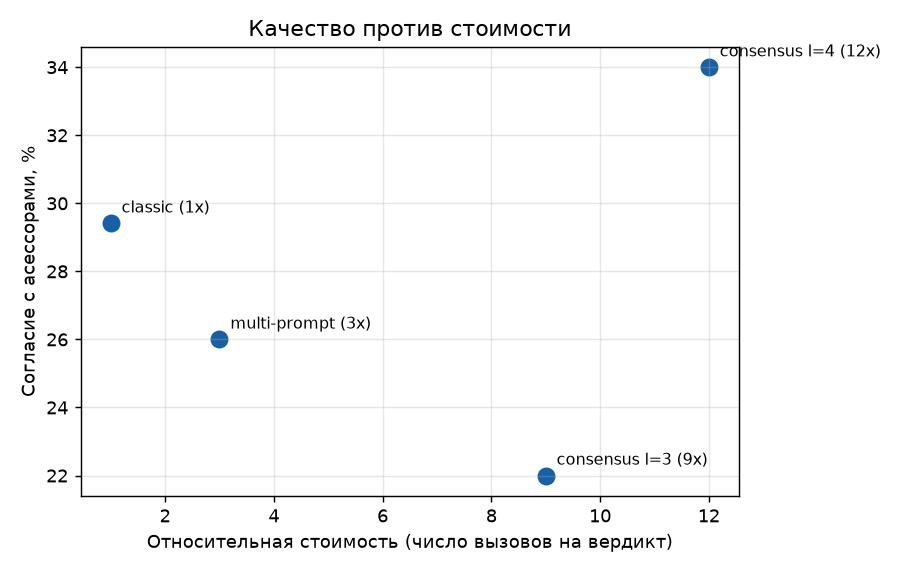
\includegraphics[width=0.8\textwidth]{figures/results-pareto.jpeg}
    \caption{Согласие с асессорами против относительной стоимости.
    Рост стоимости с $1\times$ до $12\times$ не сопровождается ростом
    согласия -- Pareto-улучшения за счёт усложнения схемы на данном наборе
    судей не наблюдается.}
    \label{fig:results-pareto}
\end{figure}

Ключевое наблюдение: \emph{прирост стоимости не конвертируется в прирост
качества}. Классическая схема стоит $1\times$, multi-prompt -- $3\times$,
consensus -- $9$--$12\times$, но согласие с асессорами при этом не растёт
(раздел~\ref{sec:results:agreement}, H2 не подтверждена), а consensus
$l{=}4$ даже значимо отклоняется от эталона. Поэтому «цена за дополнительный
пункт $\mathrm{SbS\text{-}NPS}$» (критерий~3 раздела
\ref{sec:experiments:criteria}) для перехода classic\,$\to$\,consensus
здесь \emph{не определена в положительную сторону}: за $9$--$12\times$
стоимости качество согласия не улучшается.

Единственный экономически оправданный эффект усложнения -- \emph{робастность
покрытия}: переход от одиночного судьи к multi-prompt ($3\times$) повышает
долю запросов с валидным вердиктом с $34\%$ до $100\%$
(раздел~\ref{sec:results:agreement}), устраняя хрупкость одиночного
вызова. Дальнейший рост до consensus ($9$--$12\times$) этого преимущества
уже не добавляет.

Сравнение с асессорами: даже самая дешёвая автоматическая схема на порядок
дешевле асессорской разметки (раздел~\ref{sec:experiments:cost}), но на
данном наборе судей её согласие с асессорами ($22$--$34\%$) слишком низко,
чтобы заменять разметку как источник вердиктов. Экономия реальна, но
реализуема пока только для \emph{дешёвого направленного мониторинга}
(знак $\mathrm{SbS\text{-}NPS}$), а не для замены асессорского вердикта.

\section{Рекомендации}
\label{sec:results:recommendations}

По итогам разделов~\ref{sec:results:agreement}--\ref{sec:results:economics}.

\begin{enumerate}
    \item \textbf{Не заменять асессорскую разметку} полностью: на текущем
        наборе судей согласие слишком низко, а consensus значимо
        переоценивает $\mathrm{SbS\text{-}NPS}$. Автоматическая оценка
        пригодна как дешёвый \emph{направленный} сигнал (знак различия), не
        как замена вердикта.
    \item \textbf{Для дешёвого регулярного мониторинга -- multi-prompt
        ($3\times$)}: он даёт полное покрытие (робастность) при умеренной
        стоимости, тогда как consensus ($9$--$12\times$) не окупается ни по
        согласию, ни по робастности.
    \item \textbf{Усиливать судей, а не только схему.} Узкое место --
        сила компактных открытых моделей-судей и их verbosity-смещение
        (раздел~\ref{sec:results:errors}), а не механизм агрегации.
        Приоритет -- более сильные/откалиброванные судьи и коррекция
        verbosity (например, нормировка на длину ответа).
    \item \textbf{Калибровать порог $\theta$ и набор промптов на golden
        set} и увеличить эталонную корзину до $N \approx 200$: текущая
        мощность ($N = 50$) не позволяет ни доказать эквивалентность, ни
        уверенно различить малые приросты
        (раздел~\ref{sec:experiments:power}).
    \item \textbf{Consensus -- только после коррекции смещений.} До
        устранения общего для судей перекоса (verbosity) агрегация по
        моделям усиливает, а не гасит ошибку, поэтому преждевременна.
\end{enumerate}

Эти рекомендации согласуются с центральной гипотезой работы в её
ослабленной, но честной форме: гибридные схемы повышают \emph{робастность}
автоматической оценки и сохраняют верное направление, однако согласия,
эквивалентного асессорскому, на компактных открытых судьях достичь не
удалось -- это и определяет приоритеты дальнейшей работы
(глава~\ref{sec:conclusion}).

\chapter{Заключение}
\label{sec:conclusion}

\section{Основные результаты}

В работе спроектирован и формализован воспроизводимый пайплайн оценки
мультимодальных LLM-систем на основе LLM-as-a-Judge.

\begin{enumerate}
    \item Проведён обзор существующих подходов к формализованной оценке
        LLM (глава~\ref{sec:related}): бенчмарки и датасеты,
        LLM-as-a-Judge, доменно-специфические фреймворки, требования к
        воспроизводимости и известные ограничения (смещения CALM,
        чувствительность к промпту, контаминация данных).
        На основе обзора выбраны две опорные идеи -- PRD~\cite{li2023prd}
        и multi-prompt evaluation~\cite{mizrahi2024stateofwhatart}.
    \item Формализованы метрики оценки (глава~\ref{sec:method}):
        поточечная $\mathrm{NPS}$/$\Delta\mathrm{NPS}$
        (\eqref{eq:nps}--\eqref{eq:delta-nps}) и попарная
        $\mathrm{SbS\text{-}NPS}$ с пороговым голосованием
        (\eqref{eq:vote}--\eqref{eq:sbs-nps}) и
        bootstrap-доверительным интервалом
        (раздел~\ref{sec:method:bootstrap}).
    \item Формализована гибридная схема LLM-as-a-Judge
        (раздел~\ref{sec:method:hybrid}): классическая (single-judge),
        multi-prompt (\eqref{eq:multiprompt-judges}) и consensus
        (\eqref{eq:consensus-judges}) как частные случаи одного
        механизма голосования с разным числом элементов $\set{J}_q$.
    \item Описан протокол воспроизводимости пайплайна
        (раздел~\ref{sec:method:reproducibility}): версионирование
        моделей и промптов, фиксация параметров запуска, логирование и
        повторные прогоны.
    \item Проведены эксперименты по схеме из четырёх этапов
        (раздел~\ref{sec:experiments:design}), сравнивающие
        классическую, multi-prompt и consensus схемы между собой и с
        асессорской разметкой по $\mathrm{SbS\text{-}NPS}$ и стоимости.
\end{enumerate}

\textbf{Итоговый ответ на гипотезу.}
На наборе компактных открытых моделей-судей (N=50, текстовый режим) ни multi-prompt, ни consensus-схема не показали статистически значимого роста согласия с асессорами по сравнению с single-judge (парный bootstrap, H2 не подтверждена, раздел~\ref{sec:results:agreement}). Consensus при $l=4$ значимо переоценивает $\mathrm{SbS\text{-}NPS}$ и отклоняется от асессоров (нарушение эквивалентности \eqref{eq:tost}). Единственный подтверждённый эффект -- рост робастности покрытия: переход от одиночного судьи к multi-prompt ($3\times$) повышает долю запросов с валидным вердиктом с $34\%$ до $100\%$ (раздел~\ref{sec:results:agreement}). Сила моделей-судей (verbosity bias), а не механизм агрегации, является узким местом.

\section{Научный и практический вклад}

\textbf{Научный вклад} -- единая формализация классической,
multi-prompt и consensus схем LLM-as-a-Judge как частных случаев одной
модели голосования (раздел~\ref{sec:method:hybrid}), что позволяет
сравнивать их между собой и с асессорской разметкой по единой метрике
$\mathrm{SbS\text{-}NPS}$ с доверительным интервалом, а не по
разнородным метрикам, специфичным для отдельных фреймворков
(глава~\ref{sec:related}).

\textbf{Практический вклад} -- воспроизводимый пайплайн
(раздел~\ref{sec:method:reproducibility}), позволяющий регулярно (на
каждое изменение системы или конкурента) автоматически получать
сравнение $S$ и $C$ с количественной оценкой надёжности результата, без
обязательного привлечения асессоров на каждой итерации.
По модели стоимости (раздел~\ref{sec:experiments:cost}) даже самая
дорогая из рассмотренных автоматических схем (consensus при
$l \cdot m = 9$--$12$) обходится примерно на порядок дешевле полной
асессорской разметки той же корзины, что и делает регулярные прогоны
экономически осмысленными.

\section{Ограничения}

Результаты работы следует трактовать с учётом ряда ограничений.

\begin{enumerate}
    \item \textbf{Объём выборки.} Основной текстовый эксперимент проведён
        при $N = 50$ на test-сплите (MDE $\approx 20$~п.п.), что делает
        TOST с $\delta = 10$~п.п. недостижимым для этого набора данных.
        Мультимодальный ablation study проведён при $N = 200$
        (раздел~\ref{sec:results:multimodal-ablation}), что обеспечивает
        MDE $\approx 10$~п.п. и делает TOST теоретически достижимым.
        Тем не менее TOST не достигнут ни при $N = 50$, ни при $N = 200$ --
        это свидетельствует о реальном расхождении между автоматической
        оценкой и асессорской разметкой, а не только о недостатке мощности.
    \item \textbf{Однородность судей.} Использованные модели-судьи
        принадлежат к близким семействам открытых моделей; результаты
        могут не переноситься на другие архитектуры, а самопредпочтение
        внутри одного семейства консенсус устраняет лишь частично
        (раздел~\ref{sec:related:hybrid-baselines}).
    \item \textbf{Мультимодальность сведена к скриншотам.} Визуальный
        вход судьи приводится к статичному скриншоту ответа
        (раздел~\ref{sec:experiments:pilot-multimodal}); живые
        интерактивные элементы, видео и динамические превью остаются за
        рамками и требуют отдельного исследования.
    \item \textbf{Остаточная стохастичность.} Даже при температуре $0$
        часть API недетерминирована; разброс
        $\mathrm{SbS\text{-}NPS}$ между повторными прогонами $R$
        (раздел~\ref{sec:method:reproducibility}) не равен нулю и должен
        учитываться при сравнении схем.
    \item \textbf{Порог $\theta = 0.7$ взят из литературы.} Значение
        обосновано (раздел~\ref{sec:method:sbs-nps}), но без
        индивидуальной калибровки под конкретную корзину может быть
        неоптимальным.
    \item \textbf{Межасессорская согласованность (IRR).} Коэффициент конкордации (Cohen~$\kappa$) между асессорами на golden set не измерен. Это ограничение не позволяет количественно обосновать порог $\delta = 10$~п.п. для TOST (раздел~\ref{sec:method:bootstrap:equiv}) через межасессорскую дисперсию; порог обоснован косвенно (раздел~\ref{sec:experiments:power}).
\end{enumerate}

\paragraph{Что подтверждено и что не подтверждено.}
Таблица~\ref{tab:hypotheses-summary} сводит результаты проверки гипотез.

\begin{table}[htbp]
\centering
\caption{Результаты проверки гипотез}
\label{tab:hypotheses-summary}
\begin{tabular}{p{5cm}cc}
\toprule
Гипотеза & Результат & Причина \\
\midrule
Multi-prompt $>$ classic по согласию & Не подтверждена & Недостаток мощности / verbosity bias \\
Consensus $>$ multi-prompt & Не подтверждена & Verbosity bias усиливается \\
Схемы воспроизводят направление асессоров & Подтверждена & Знак $\mathrm{SbS\text{-}NPS}$ совпадает \\
Агрегация повышает робастность покрытия & Подтверждена & $34\% \to 100\%$ валидных вердиктов \\
\bottomrule
\end{tabular}
\end{table}

\section{Направления дальнейшей работы}

\begin{itemize}
    \item Итеративная дискуссия между судьями (полная схема
        PRD~\cite{li2023prd}) вместо одноразового консенсуса
        \eqref{eq:consensus-judges} -- оценка прироста согласия
        относительно роста стоимости.
    \item Адаптивное перекрытие $\abs{\set{J}_q}$: увеличение числа
        судей только для запросов с неоднозначным голосованием (близким
        к порогу $\theta$ в \eqref{eq:verdict}), снижающее среднюю
        стоимость по сравнению с фиксированным $l \cdot m$.
    \item Автоматическая калибровка порога $\theta$ и набора промптов
        $p_1, \dots, p_M$ по golden set
        (раздел~\ref{sec:method:data}) как часть пайплайна, а не как
        ручной шаг.
    \item Перенос формализации
        (раздел~\ref{sec:method:hybrid}) на мультимодальных судей,
        включая специфичные для изображений и видео типы смещений,
        отмеченные в MLLM-as-a-Judge~\cite{chen2024mllmjudge}.
    \item Регулярное обновление корзины $\set{Q}$ по аналогии с
        LiveBench~\cite{white2024livebench} для снижения риска
        контаминации и устаревания golden set.
    \item Интеграция пайплайна с практиками MLOps: автоматическое
        версионирование моделей, промптов и корзин, регистрация прогонов
        и метрик, регрессионные алерты на просадку
        $\mathrm{SbS\text{-}NPS}$ -- доведение протокола
        воспроизводимости (раздел~\ref{sec:method:reproducibility}) до
        непрерывного процесса оценки.
\end{itemize}


\backmatter

\chapter*{Приложение A. Тексты промптов судьи}
\addcontentsline{toc}{chapter}{Приложение A}
\label{app:prompts}

Все три промпта реализуют одну задачу — попарную оценку ответов
системы $S$ и конкурента $C$ по четырём критериям чеклиста
(Relevance $\to$ Accuracy $\to$ Completeness $\to$ Readability).
Различие — в глубине инструкции и наличии примеров.

\section{Промпт c1\_compact (компактный, zero-shot)}
\label{app:compact}

Назначение: минимальная инструкция, судья выставляет
чекбоксы напрямую без явного рассуждения.

Стратегия генерации: zero-shot, temperature$=0{,}0$.

\begin{verbatim}
[SYSTEM]
Ты — эксперт по оценке качества ответов
диалоговых ассистентов.

[USER]
Запрос пользователя:
{query}

Ответ системы A:
{response_S}

Ответ системы B:
{response_C}

Оцени каждый ответ строго по порядку.
Для каждого критерия укажи true/false.
При первом false последующие критерии
автоматически считаются false.

Критерии (в порядке проверки):
1. Relevance: отвечает ли ответ на запрос в целом?
2. Accuracy: фактически верен ли ответ
   во всех модальностях?
3. Completeness: полностью ли покрыт запрос,
   с нужным форматом и деталями?
4. Readability: структурирован и читаем ли ответ?

Формат вывода (строго JSON):
{{
  "A": {{"relevance": bool, "accuracy": bool,
        "completeness": bool, "readability": bool}},
  "B": {{"relevance": bool, "accuracy": bool,
        "completeness": bool, "readability": bool}}
}}
\end{verbatim}

\section{Промпт c2\_stoprule (явное правило «стоп»)}
\label{app:stoprule}

Назначение: явная инструкция «стоп на первом false»
снижает неоднородность интерпретации чеклиста.

Стратегия генерации: zero-shot, temperature$=0{,}0$.

\begin{verbatim}
[SYSTEM]
Ты — эксперт по оценке качества ответов
диалоговых ассистентов.

[USER]
Запрос пользователя:
{query}

Ответ системы A:
{response_S}

Ответ системы B:
{response_C}

ВАЖНО: проверяй критерии строго по порядку.
Как только критерий получает false —
все последующие автоматически false.
Не оценивай длину ответа как показатель качества:
короткий точный ответ НЕ хуже длинного.

Критерии:
1. Relevance
2. Accuracy
3. Completeness
4. Readability

Формат вывода (строго JSON):
{{
  "A": {{"relevance": bool, "accuracy": bool,
        "completeness": bool, "readability": bool}},
  "B": {{"relevance": bool, "accuracy": bool,
        "completeness": bool, "readability": bool}}
}}
\end{verbatim}

\section{Промпт c3\_reason (цепочка рассуждений, few-shot)}
\label{app:reason}

Назначение: явное рассуждение по каждому критерию
перед вынесением вердикта (перенос идеи EvalPlanner).

Стратегия генерации: few-shot (1 пример), temperature$=0{,}0$.

\begin{verbatim}
[SYSTEM]
Ты — эксперт по оценке качества ответов
диалоговых ассистентов.

[USER — FEW-SHOT ПРИМЕР]
Запрос: «Покажи график цены акции за год»

Ответ A: «Вот график: [изображение]»
Ответ B: «Цена акции росла в течение года.»

Рассуждение:
- Relevance A: ответ содержит запрошенный график → true
- Relevance B: ответ описывает тренд словами,
  без графика → false; дальнейшие критерии false

Итог:
{{"A": {{"relevance": true, "accuracy": true,
       "completeness": true, "readability": true}},
 "B": {{"relevance": false, "accuracy": false,
       "completeness": false, "readability": false}}}}

[USER — РЕАЛЬНЫЙ ЗАПРОС]
Запрос пользователя:
{query}

Ответ системы A:
{response_S}

Ответ системы B:
{response_C}

Сначала напиши рассуждение по каждому критерию
для каждого ответа (1–2 предложения на критерий).
Затем выведи итоговый JSON в том же формате,
что в примере выше.
\end{verbatim}


\printbib

\end{document}
